\chapter{Стабилизация маятника: регуляторы с заданной степенью устойчивости}
\label{ch:chap4}


\section{Синтез регулятора по состоянию}


С помощью решения линейного матричного неравенства Ляпунова для экспоненциальной устойчивости 
\begin{equation}
    \begin{cases}
        PA^T+AP+2 \alpha P + Y^T B^T+BY \preceq 0,\\
        K = Y P^+
    \end{cases}
\end{equation}

произведем расчет регулятора $u=Kx$, основываясь на линейной модели (\ref{1_model_lin}) и выбранной желаемой степенью устойчивости $\alpha =1 $ замкнутой системой.

\begin{equation}
    K = \begin{bmatrix}
        3064 & 4364 & -26684 & -11174
    \end{bmatrix}
\end{equation}

График вектора состояния представлен на рисунке \ref{4_1_1}.

\begin{figure}[!h]
\center{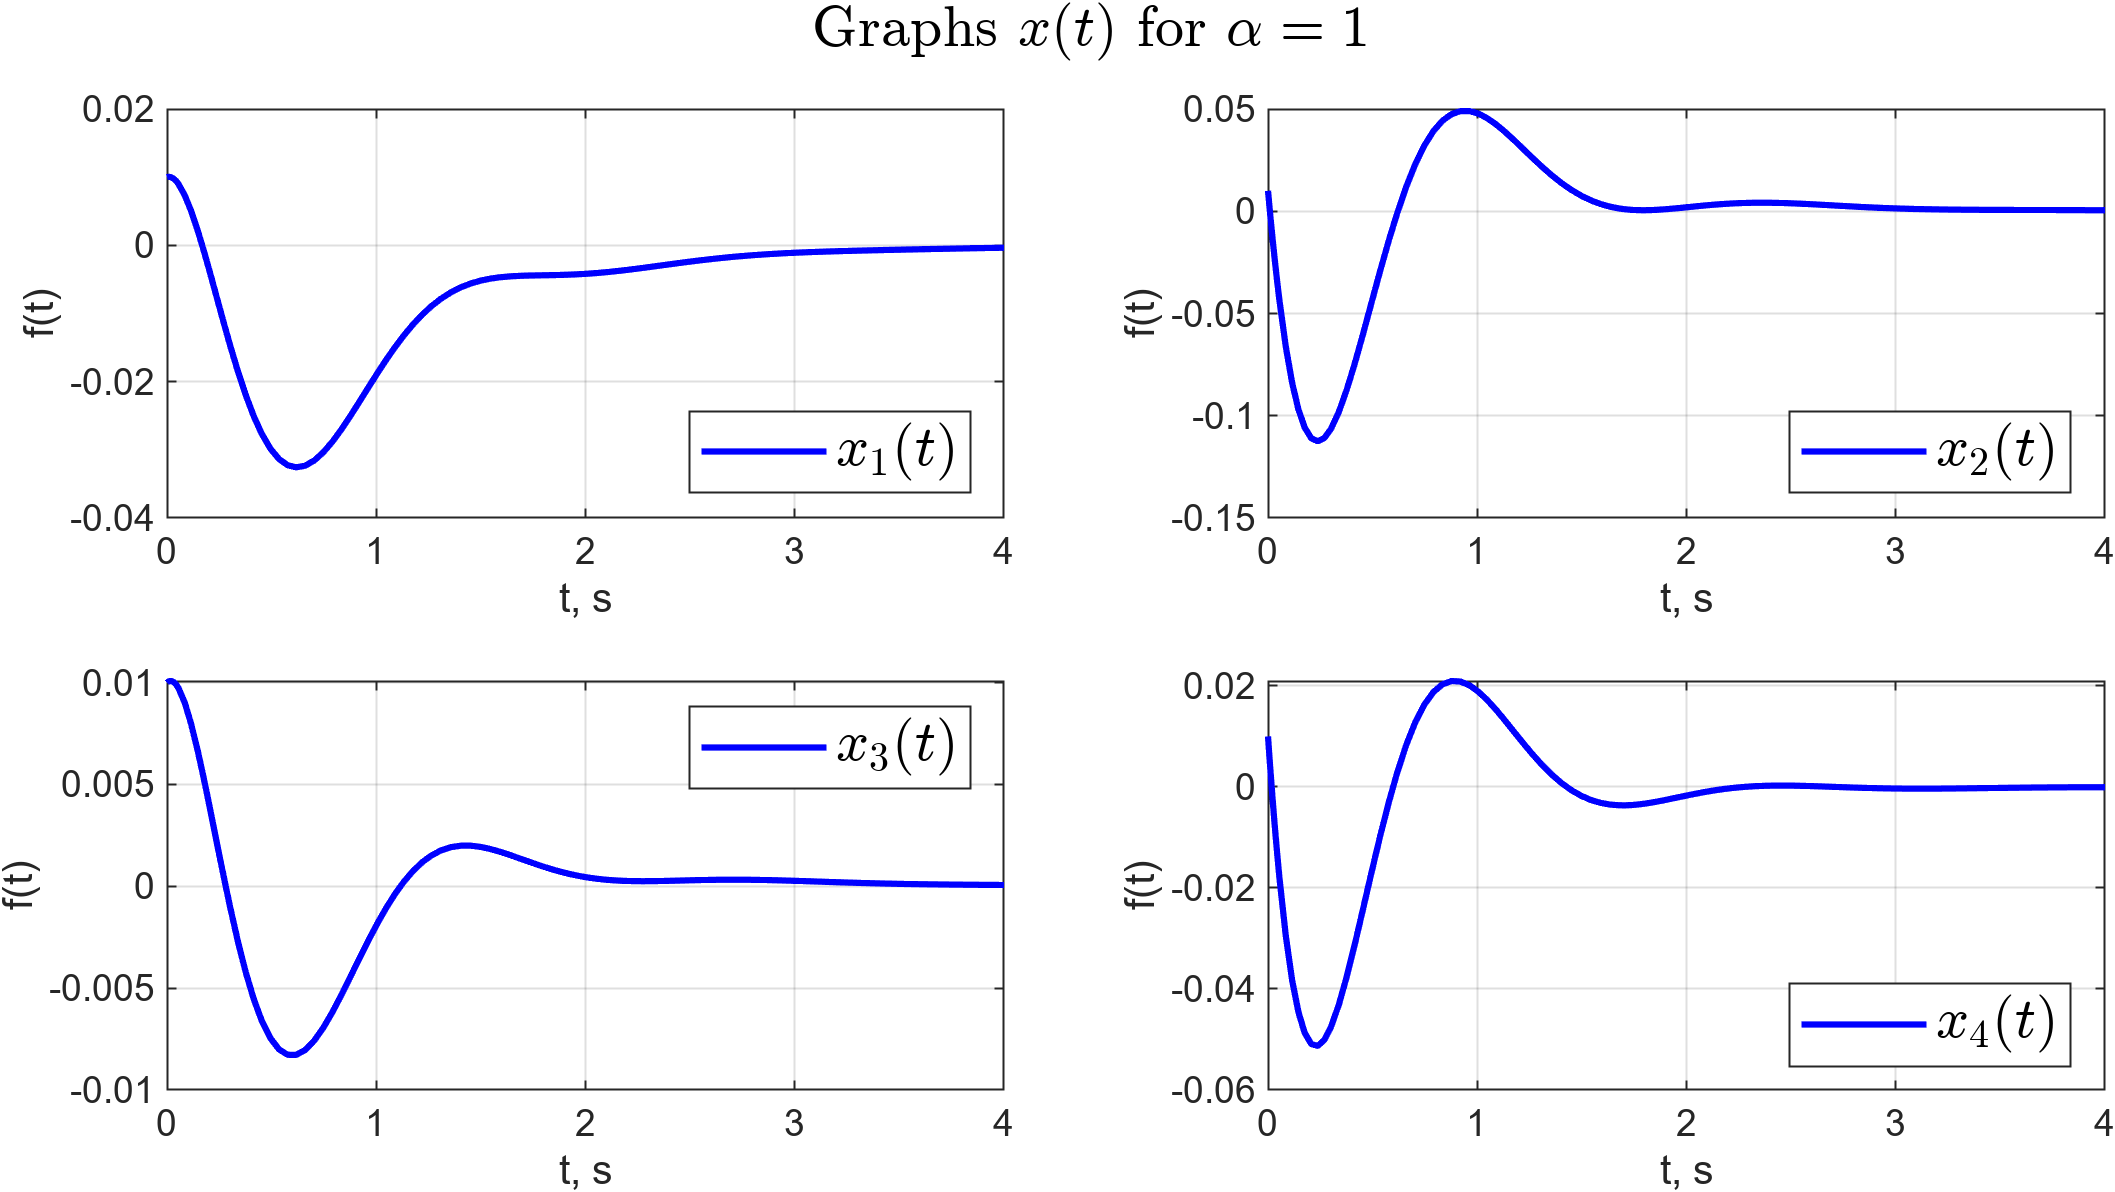
\includegraphics[width=1\linewidth]{pic/4_1_1.png}}
\caption{Графики $x(t)$, при $\alpha = 1$ и $x(0) = [0.01\, \, \,  0.01\, \, \, 0.01\, \, \, 0.01]^T$.}
\label{4_1_1}
\end{figure}






Исследуем работоспособность синтезированного регулятора при управлении нелинейной системой (\ref{1_model_full}) в зависимости от начальных условий:

\begin{equation*}
  \begin{matrix}
      x(0) = \begin{bmatrix}
          0.01 & 3 & 0.01 & 0.01
      \end{bmatrix}, & x(0) = \begin{bmatrix}
          0.01 & 0.01 & 0.01 & 1.5
      \end{bmatrix},\\
      x(0) = \begin{bmatrix}
          0.01 & 0.01 & \pi /6 & 0.01
      \end{bmatrix}, & x(0) = \begin{bmatrix}
          5 & 0.01 & 0.01 & 0.1
      \end{bmatrix},\\ 
 \end{matrix}
\end{equation*}

\begin{figure}[!h]
\center{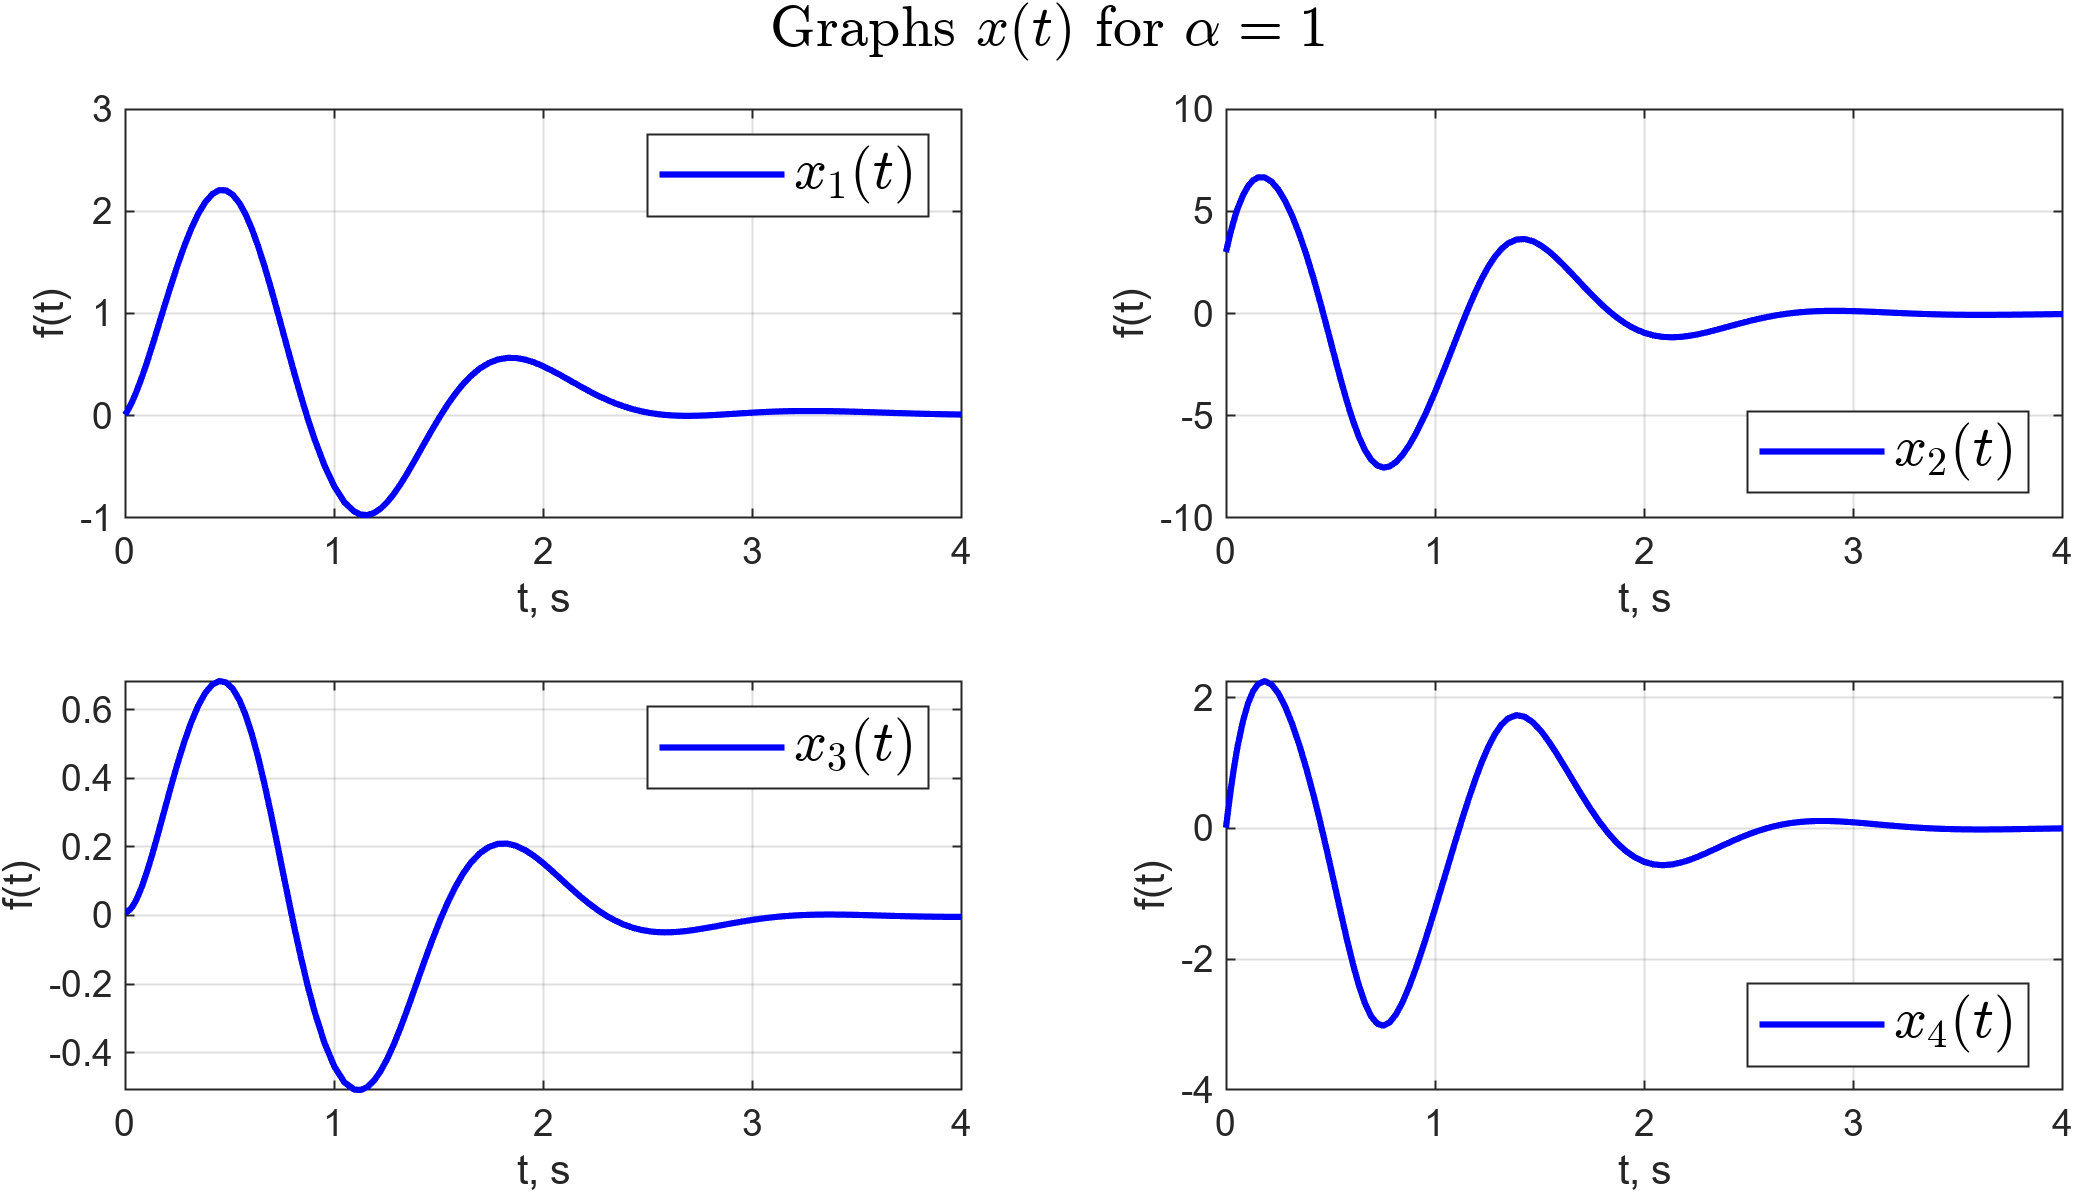
\includegraphics[width=1\linewidth]{pic/4_1_2.png}}
\caption{Графики $x(t)$, при $\alpha = 1$ и $x(0) = [0.01\, \, \,  3\, \, \, 0.01\, \, \, 0.01]^T$.}
\label{4_1_2}
\end{figure}

Заметим, что при увеличении начального значения линейной скорости до 3 м/с (рисунок \ref{4_1_2}), амплитуда компонент $x_i(t)$ возрастает примерно в 100 раз относительно начального значения 0.01 м/с.

Заметим, что при начальном значении угла отклонения маятника $\pi / 6$ регулятор еще стабилизирует систему (рисунок \ref{4_1_4}). Также видно, что для всех наборов начальных условий, вектор состояния системы становится визуально неотличим от нуля за одно и то же время $t \approx 3.5$ с. Начальные условия в данном случае влияют на амплитуду и частоту колебаний компонент вектора состояния системы.

Также начальные условия выбраны неслучайно: это максимальные значения, при которых моделирование отрабатывает за время меньше минуты -- для больших значений начальных условий не удается получить графики.

\begin{figure}[!h]
\center{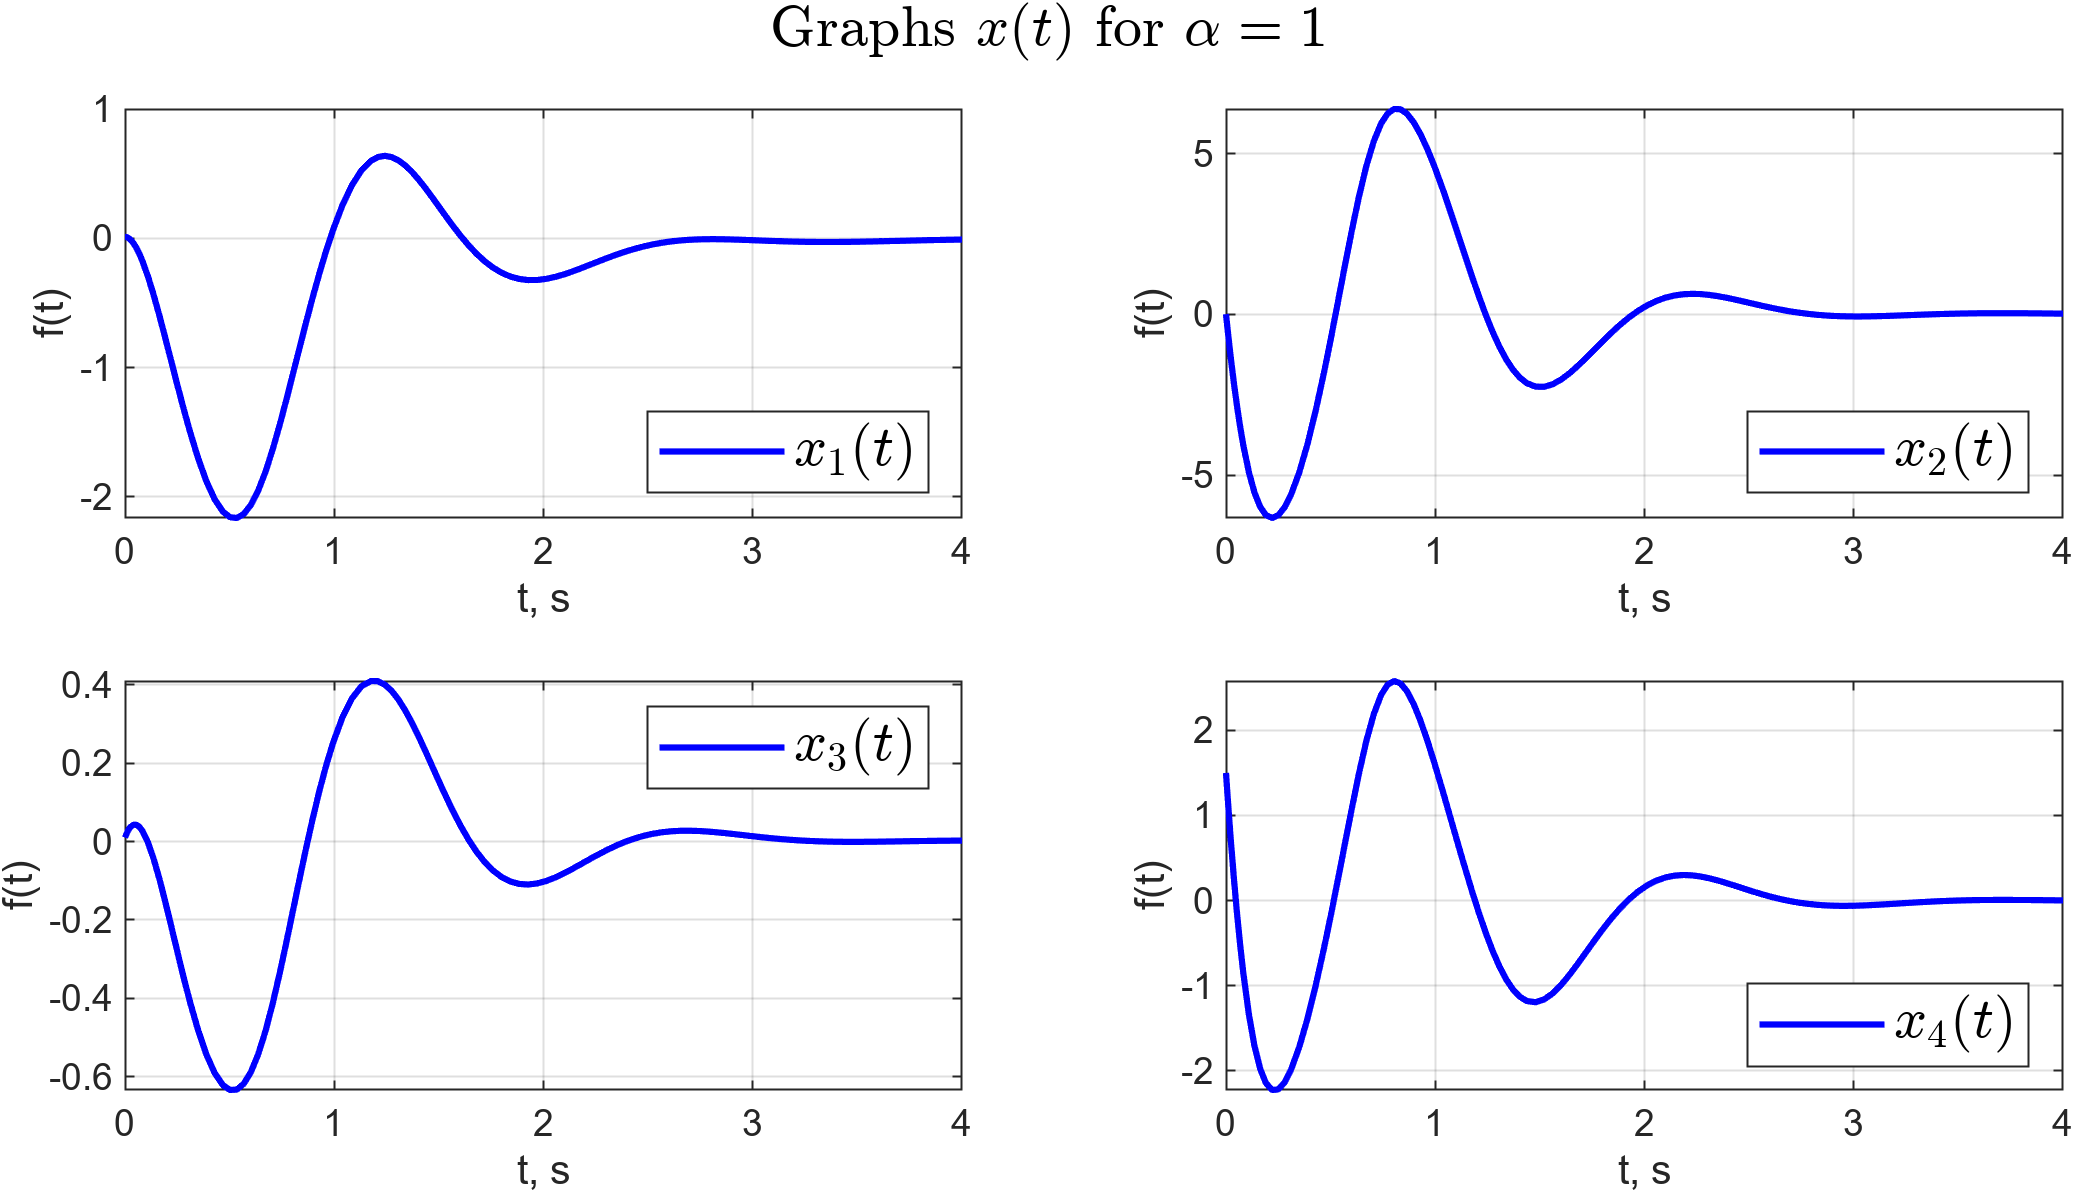
\includegraphics[width=1\linewidth]{pic/4_1_3.png}}
\caption{Графики $x(t)$, при $\alpha = 1$ и $x(0) = [0.01\, \, \,  0.01\, \, \, 0.01\, \, \, 1.5]^T$.}
\label{4_1_3}
\end{figure}


\begin{figure}[!h]
\center{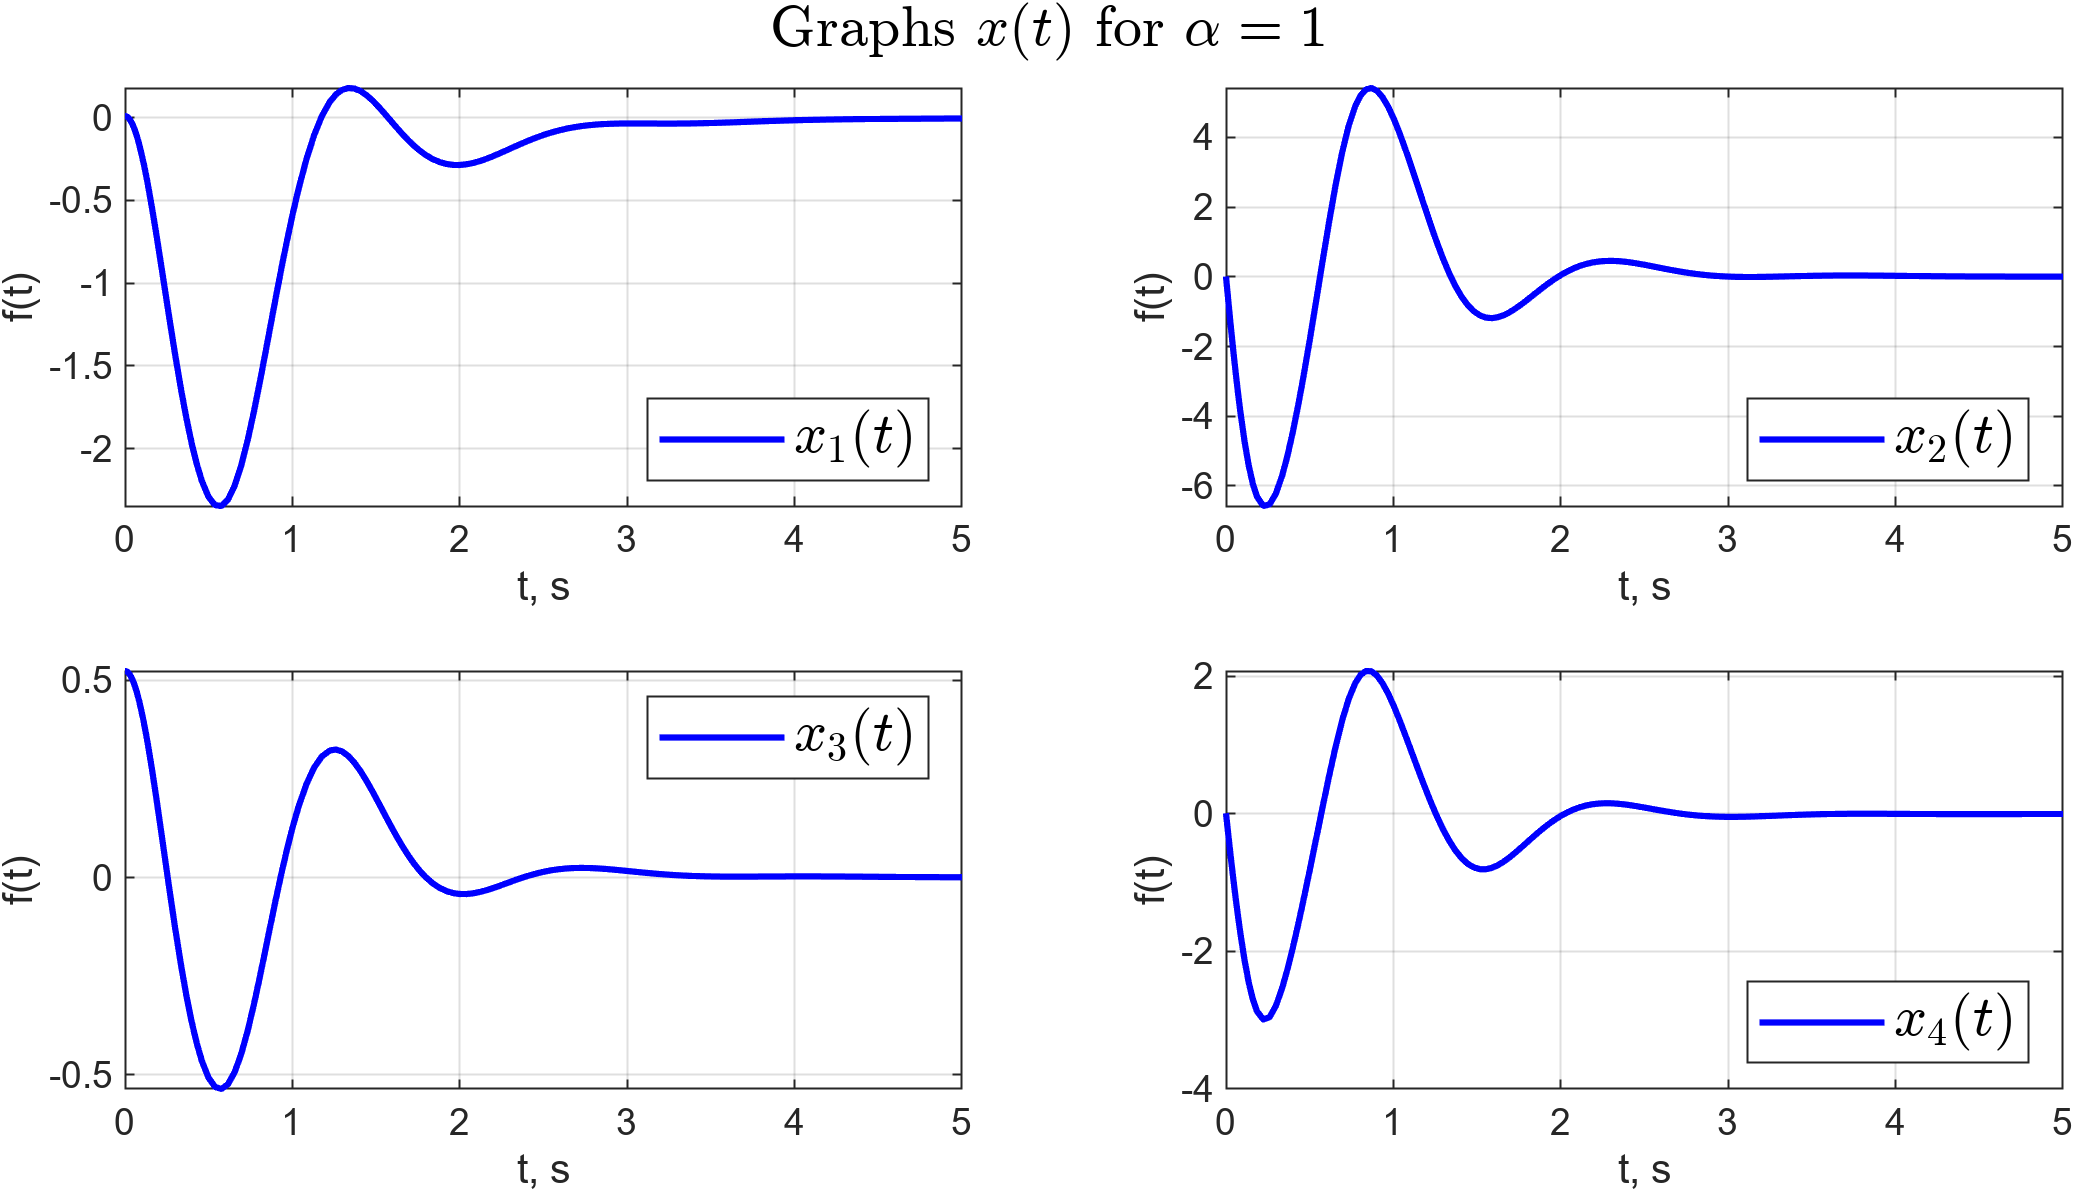
\includegraphics[width=1\linewidth]{pic/4_1_4.png}}
\caption{Графики $x(t)$, при $\alpha = 1$ и $x(0) = [0.01\, \, \,  0.01\, \, \, \pi/6\, \, \, 0.01]^T$.}
\label{4_1_4}
\end{figure}

\begin{figure}[!h]
\center{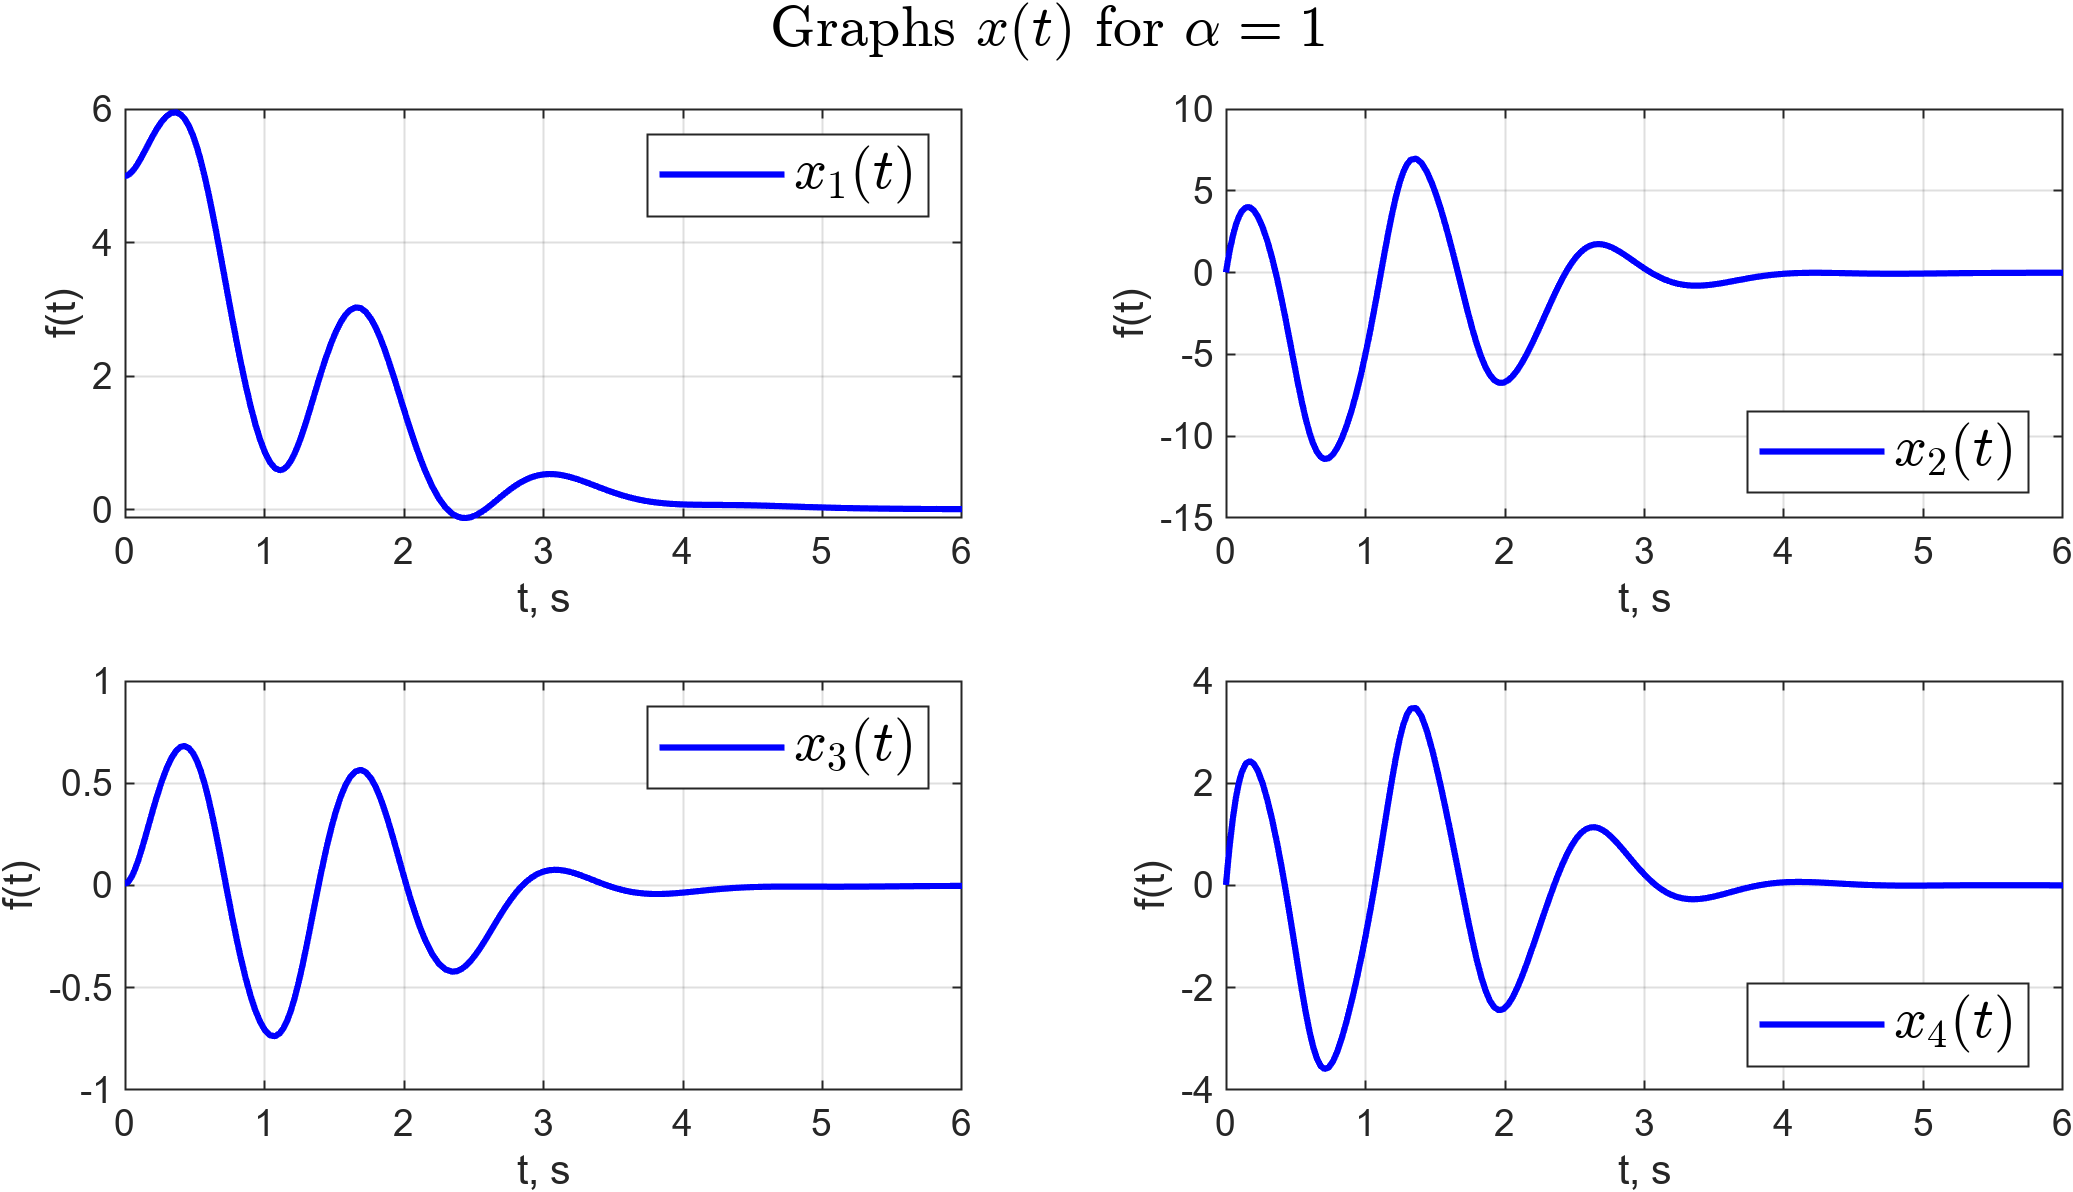
\includegraphics[width=1\linewidth]{pic/4_1_5.png}}
\caption{Графики $x(t)$, при $\alpha = 1$ и $x(0) = [5\, \, \,  0.01\, \, \, 0.01\, \, \, 0.01]^T$.}
\label{4_1_5}
\end{figure}

\section{Исследование регулятора по состоянию}

Исследуем влияние параметра $\alpha$ на максимальное отклонение маятника от вертикали, максимальное горизонтальное смещение тележки и максимальное значение управляющего сигнала при управлении нелинейной системой (\ref{1_model_full}).

 Моделирование выполнено при начальных условиях $x(0) = [0.01\, \, \,  0.01\, \, \, 0.01\, \, \, 0.01]^T$, результаты представлены в таблице \ref{4_tab_2}.


\begin{table}[h]
\centering
\caption{Результаты моделирования при разных значениях параметра $\alpha$.}
\label{4_tab_2}
\begin{tabular}{ccccc}
\toprule
$\alpha$ & $\max |\varphi|$ & $\max |a|$ & $\max |u|$ \\
\midrule
0.1  &  0.011  &  0.16  &  66  \\
0.5  &  0.01  &  0.04  &  246  \\
1 &  0.01  &  0.03  &  304  \\
2  &  0.01  &  0.025 &  942  \\
3  &  0.01  &  0.03 &  2240  \\
5  &  0.02  &  0.04 &  4732  \\
10  &  0.06  &  0.11 &  79007  \\
\bottomrule
\end{tabular}
\end{table}

Данные таблицы \ref{4_tab_2} демонстрируют сначала уменьшение максимального горизонтального смещения тележки и максимального отклонения маятника от вертикали, при $\alpha=2$ (рисунок \ref{4_2_x_2}) достигается минимум этих показателей, при дальнейшем увеличении $\alpha$ наблюдается их возрастание. Результаты моделирования представлены на рисунках \ref{4_2_x_01}-\ref{4_2_u_10}.

Максимальное значение управляющего сигнала с ростом $\alpha$ также возрастает.

\begin{figure}[!h]
	\center{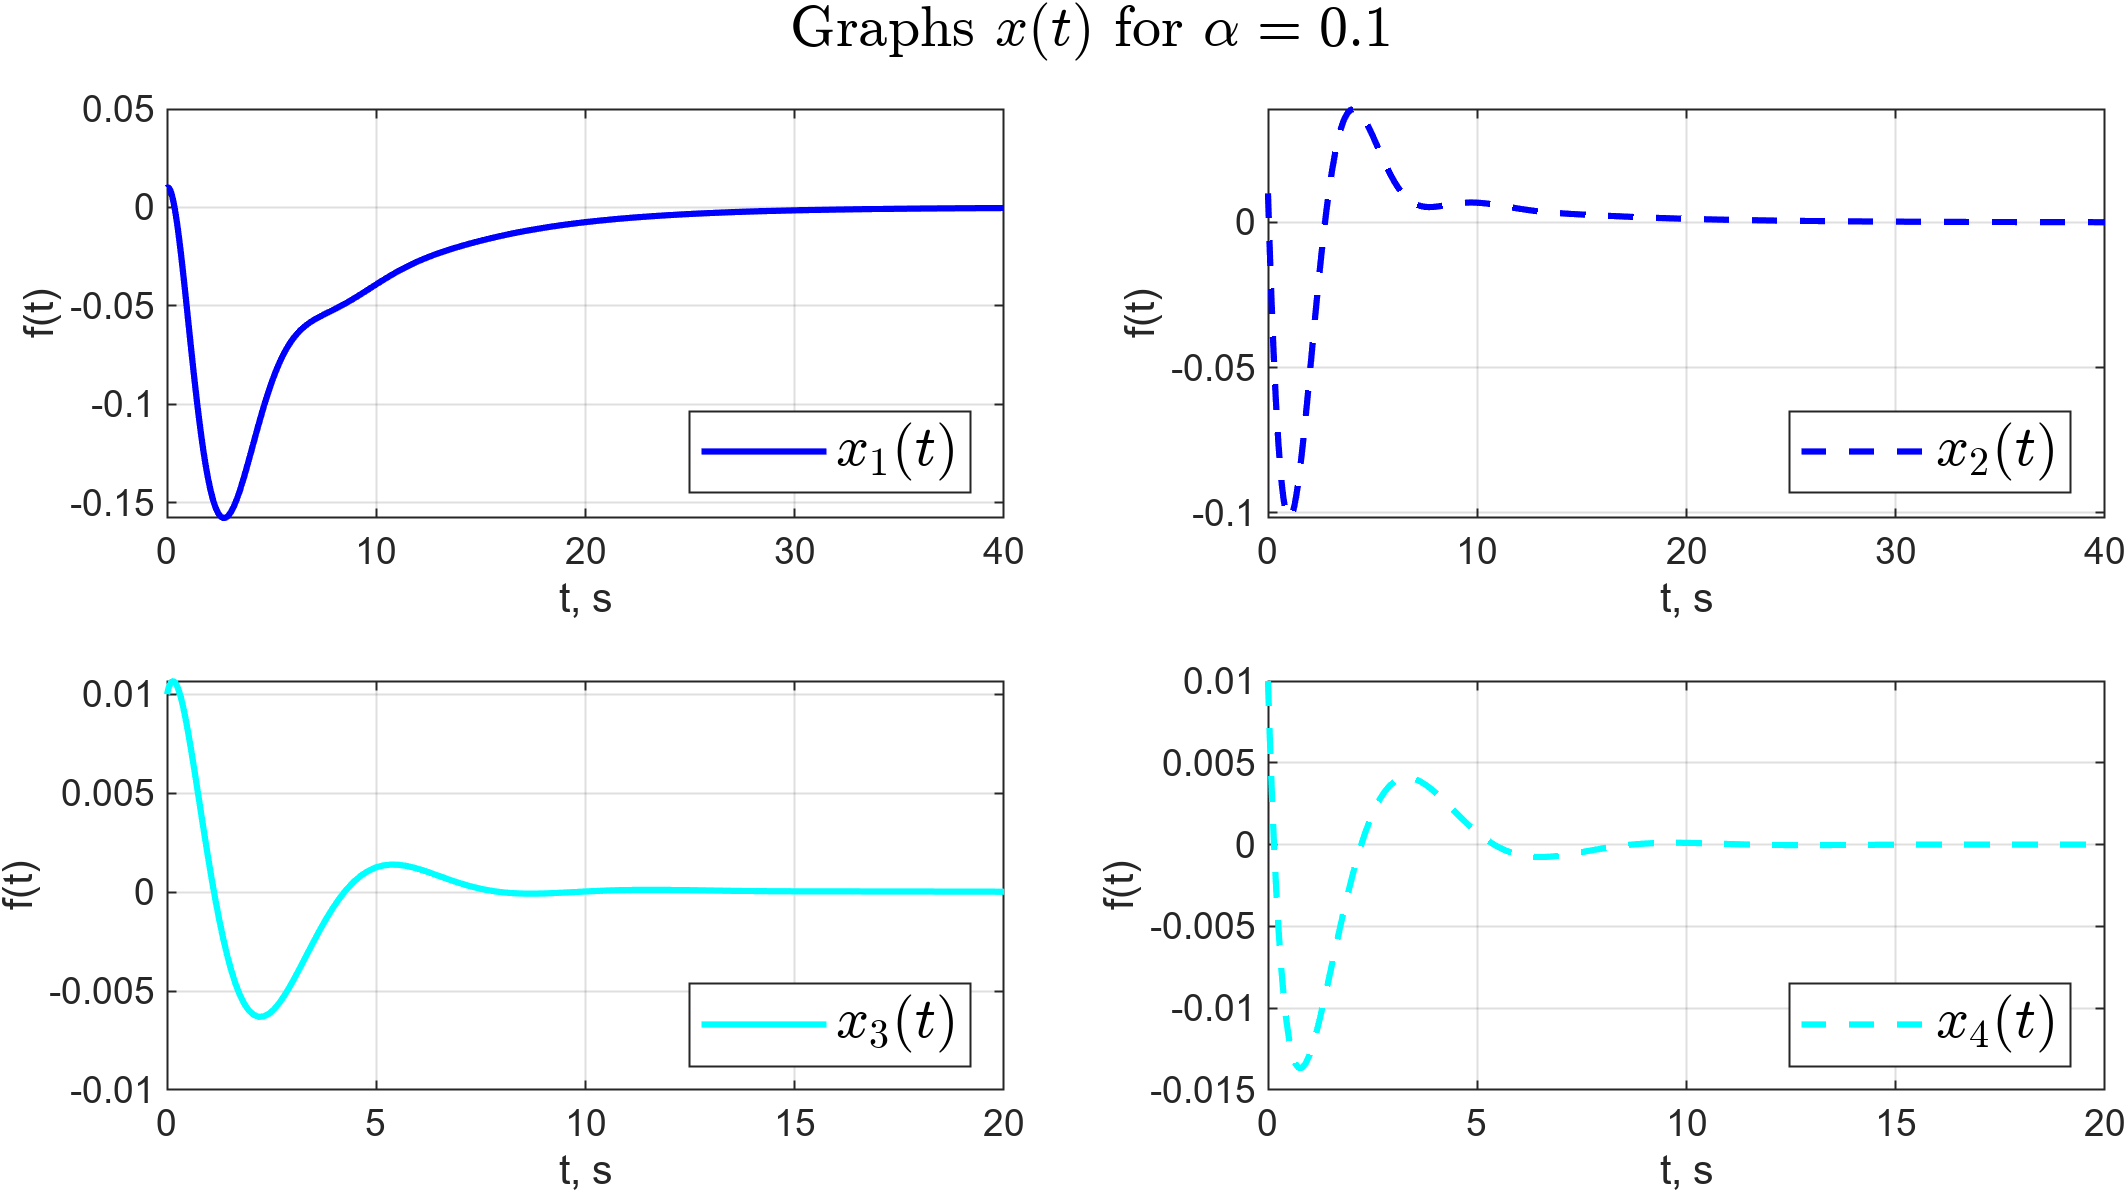
\includegraphics[width=1\linewidth]{pic_fix/4_2_x_01.png}}
	\caption{Графики вектора состояния системы при $\alpha = 0.1$.}
	\label{4_2_x_01}
\end{figure}

\begin{figure}[!h]
	\center{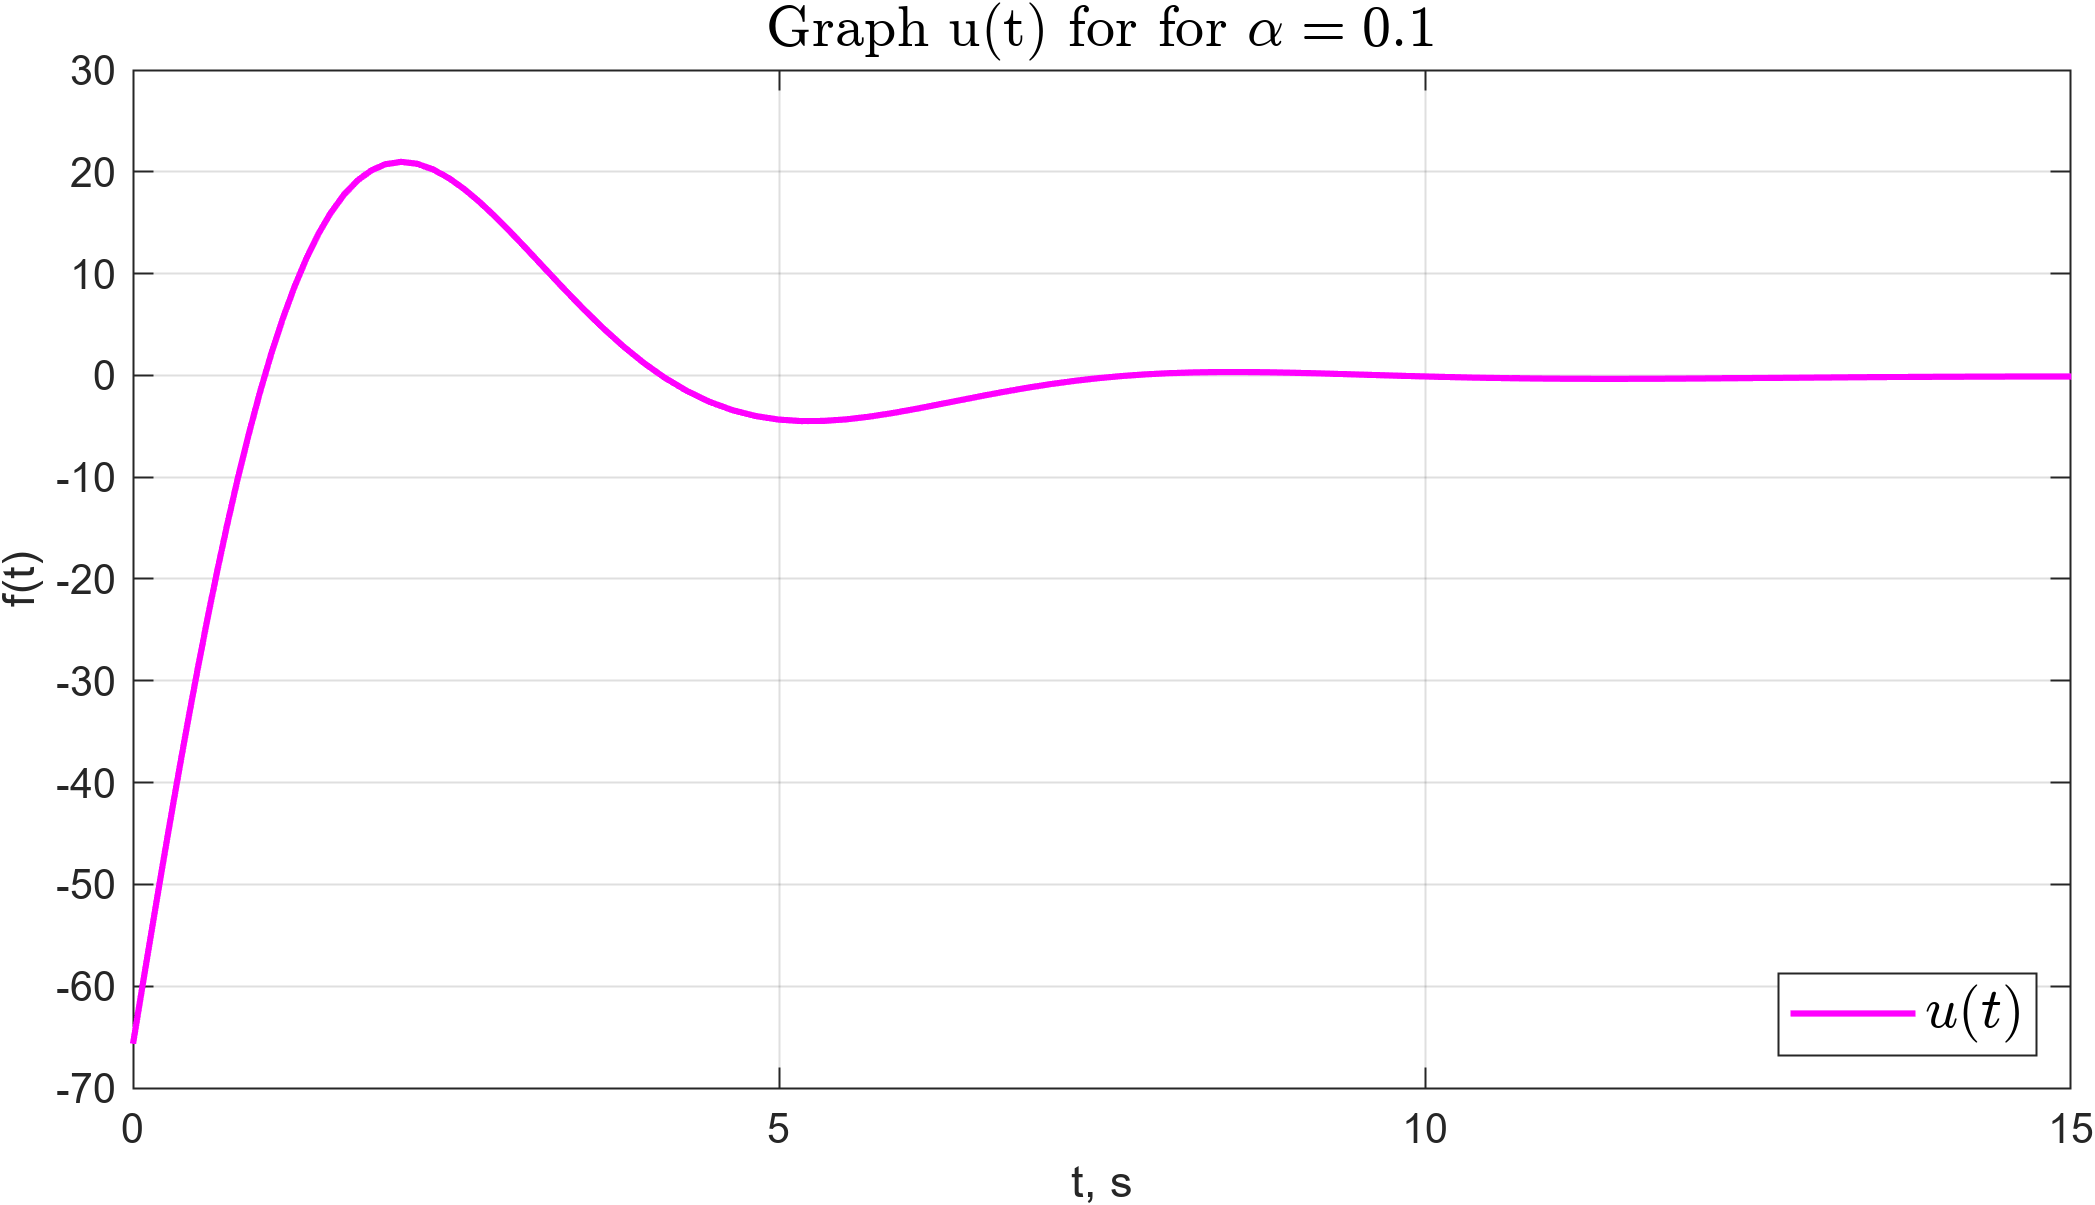
\includegraphics[width=1\linewidth]{pic_fix/4_2_u_01.png}}
	\caption{График $u(t)$ при $\alpha = 0.1$.}
	\label{4_2_u_01}
\end{figure}

\begin{figure}[!h]
	\center{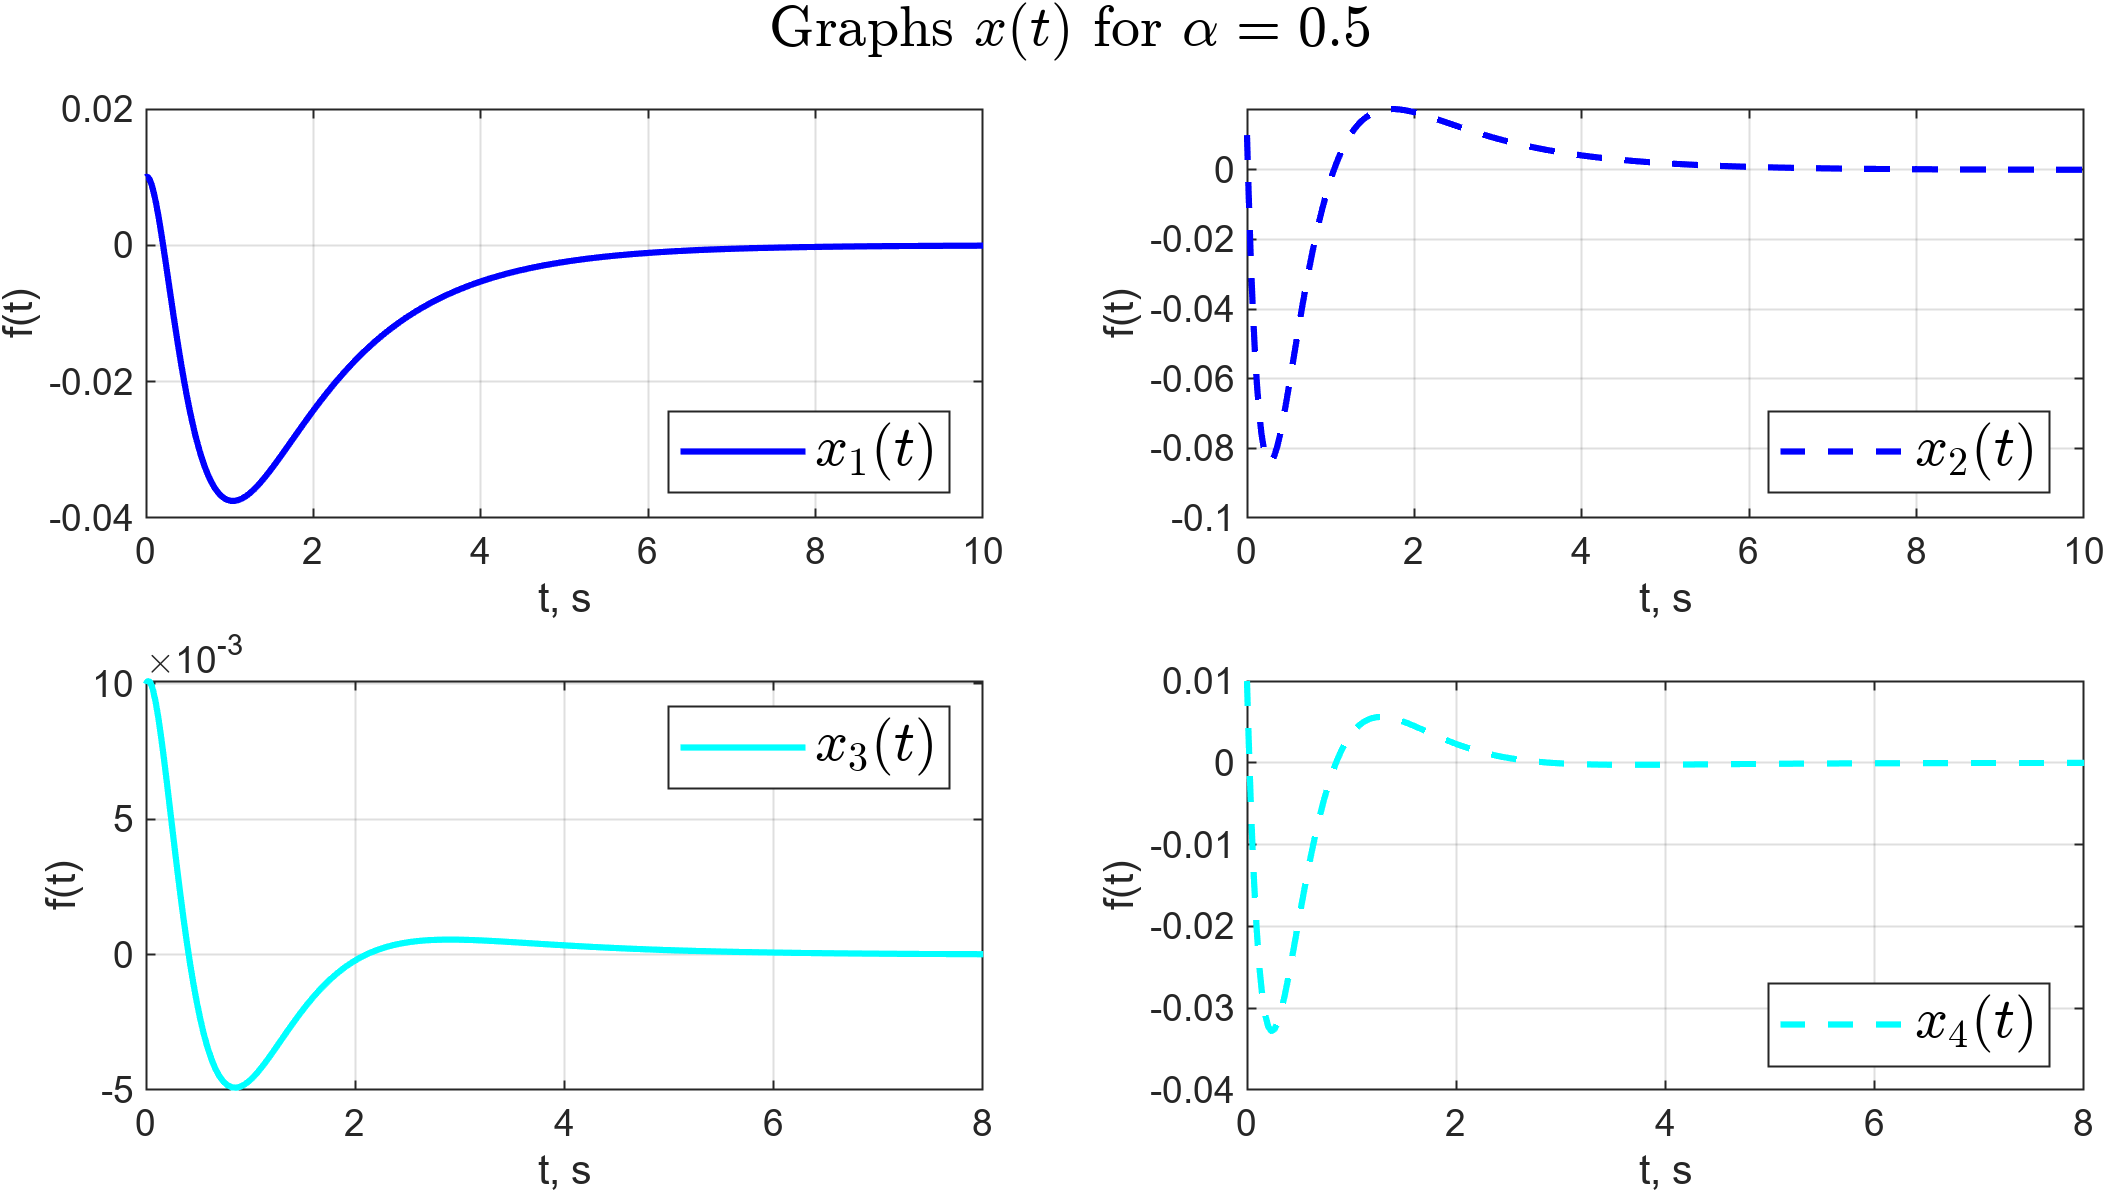
\includegraphics[width=1\linewidth]{pic_fix/4_2_x_05.png}}
	\caption{Графики вектора состояния системы при $\alpha = 0.5$.}
	\label{4_2_x_05}
\end{figure}

\begin{figure}[!h]
	\center{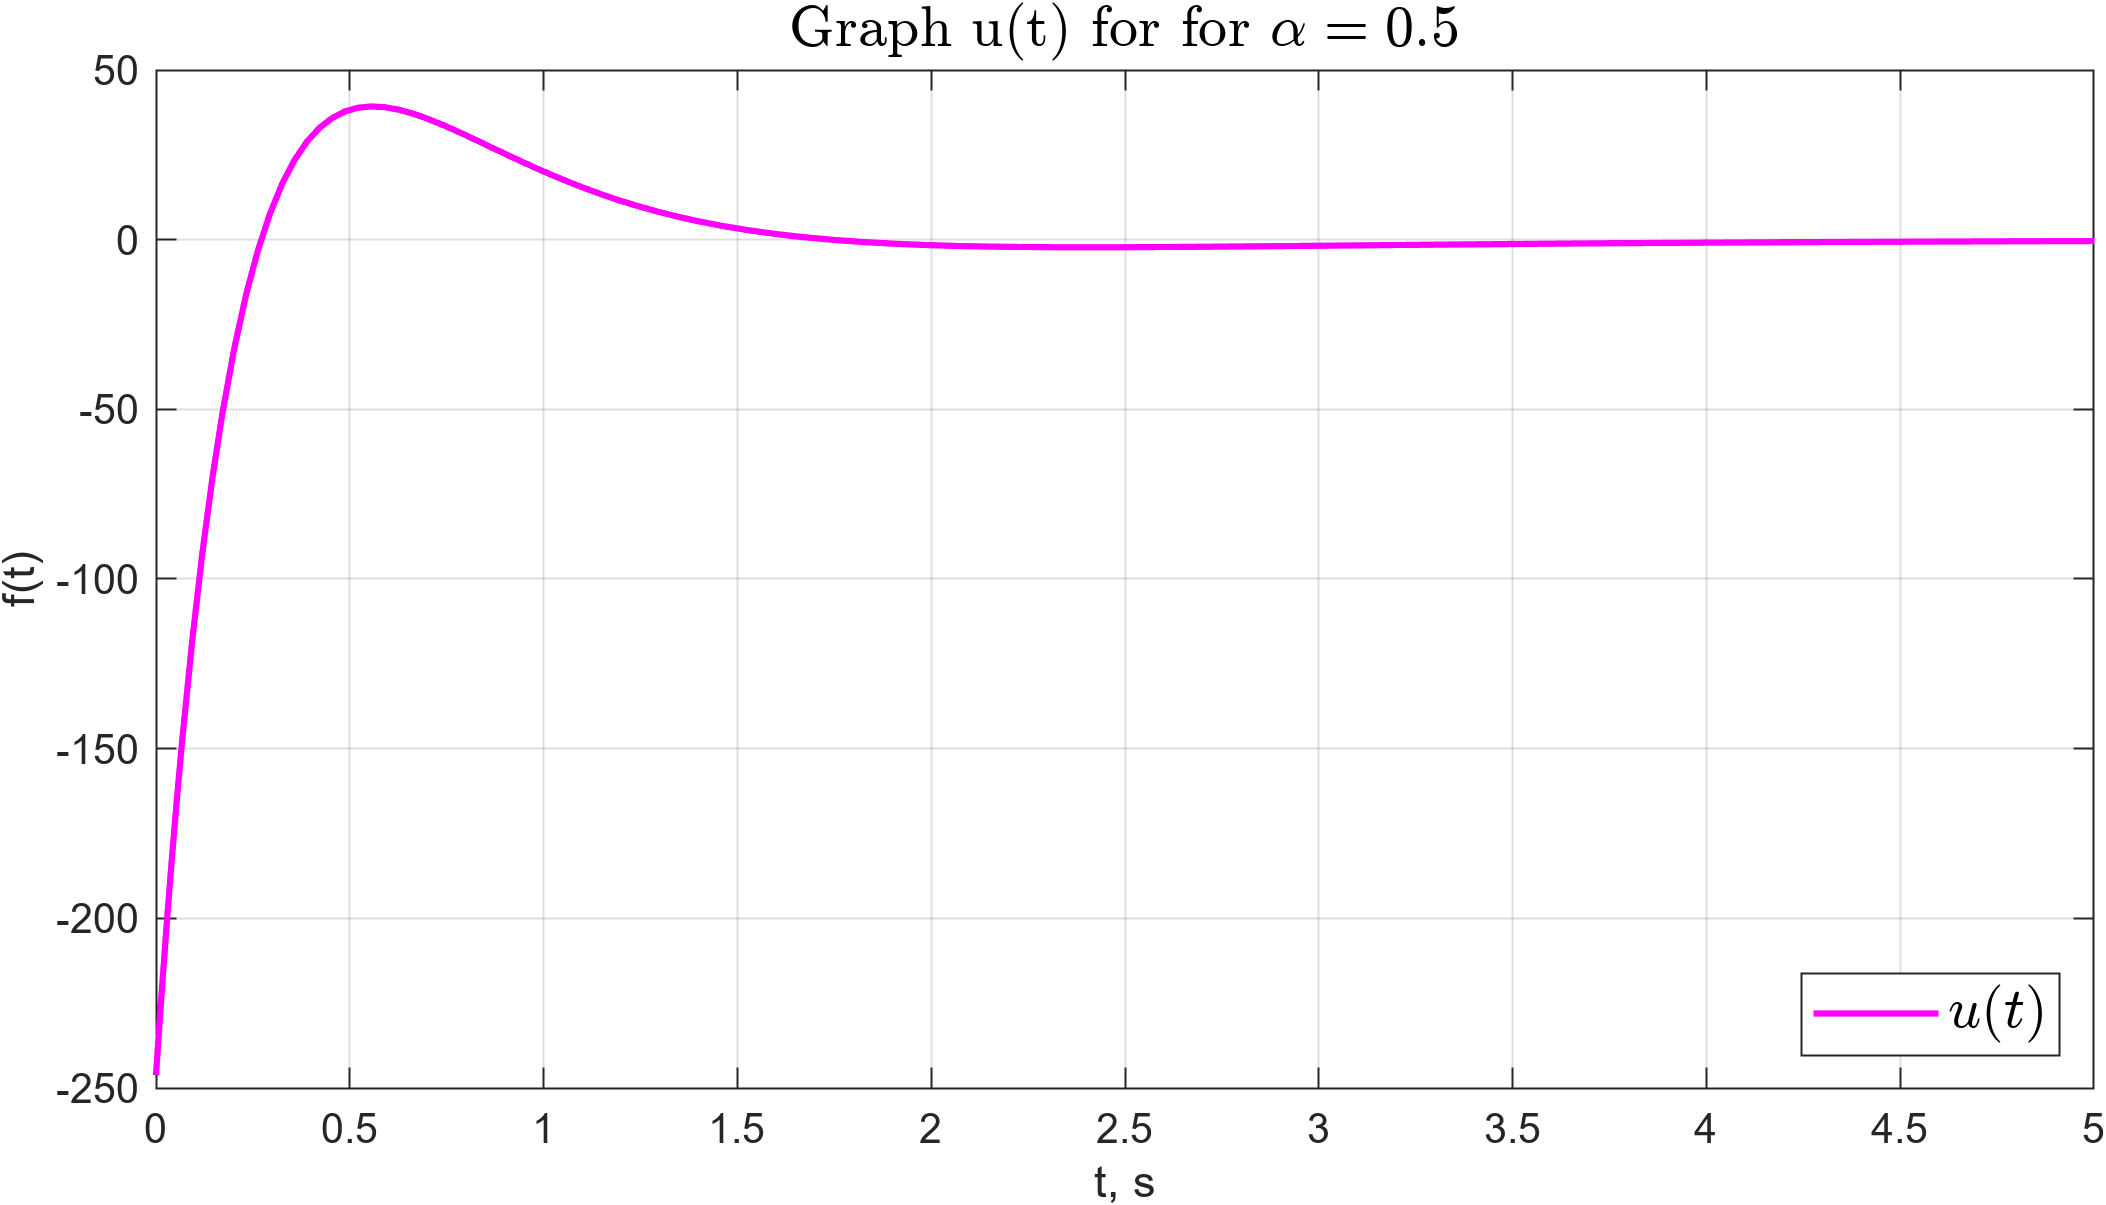
\includegraphics[width=1\linewidth]{pic_fix/4_2_u_05.png}}
	\caption{График $u(t)$ при $\alpha = 0.5$.}
	\label{4_2_u_05}
\end{figure}

\begin{figure}[!h]
	\center{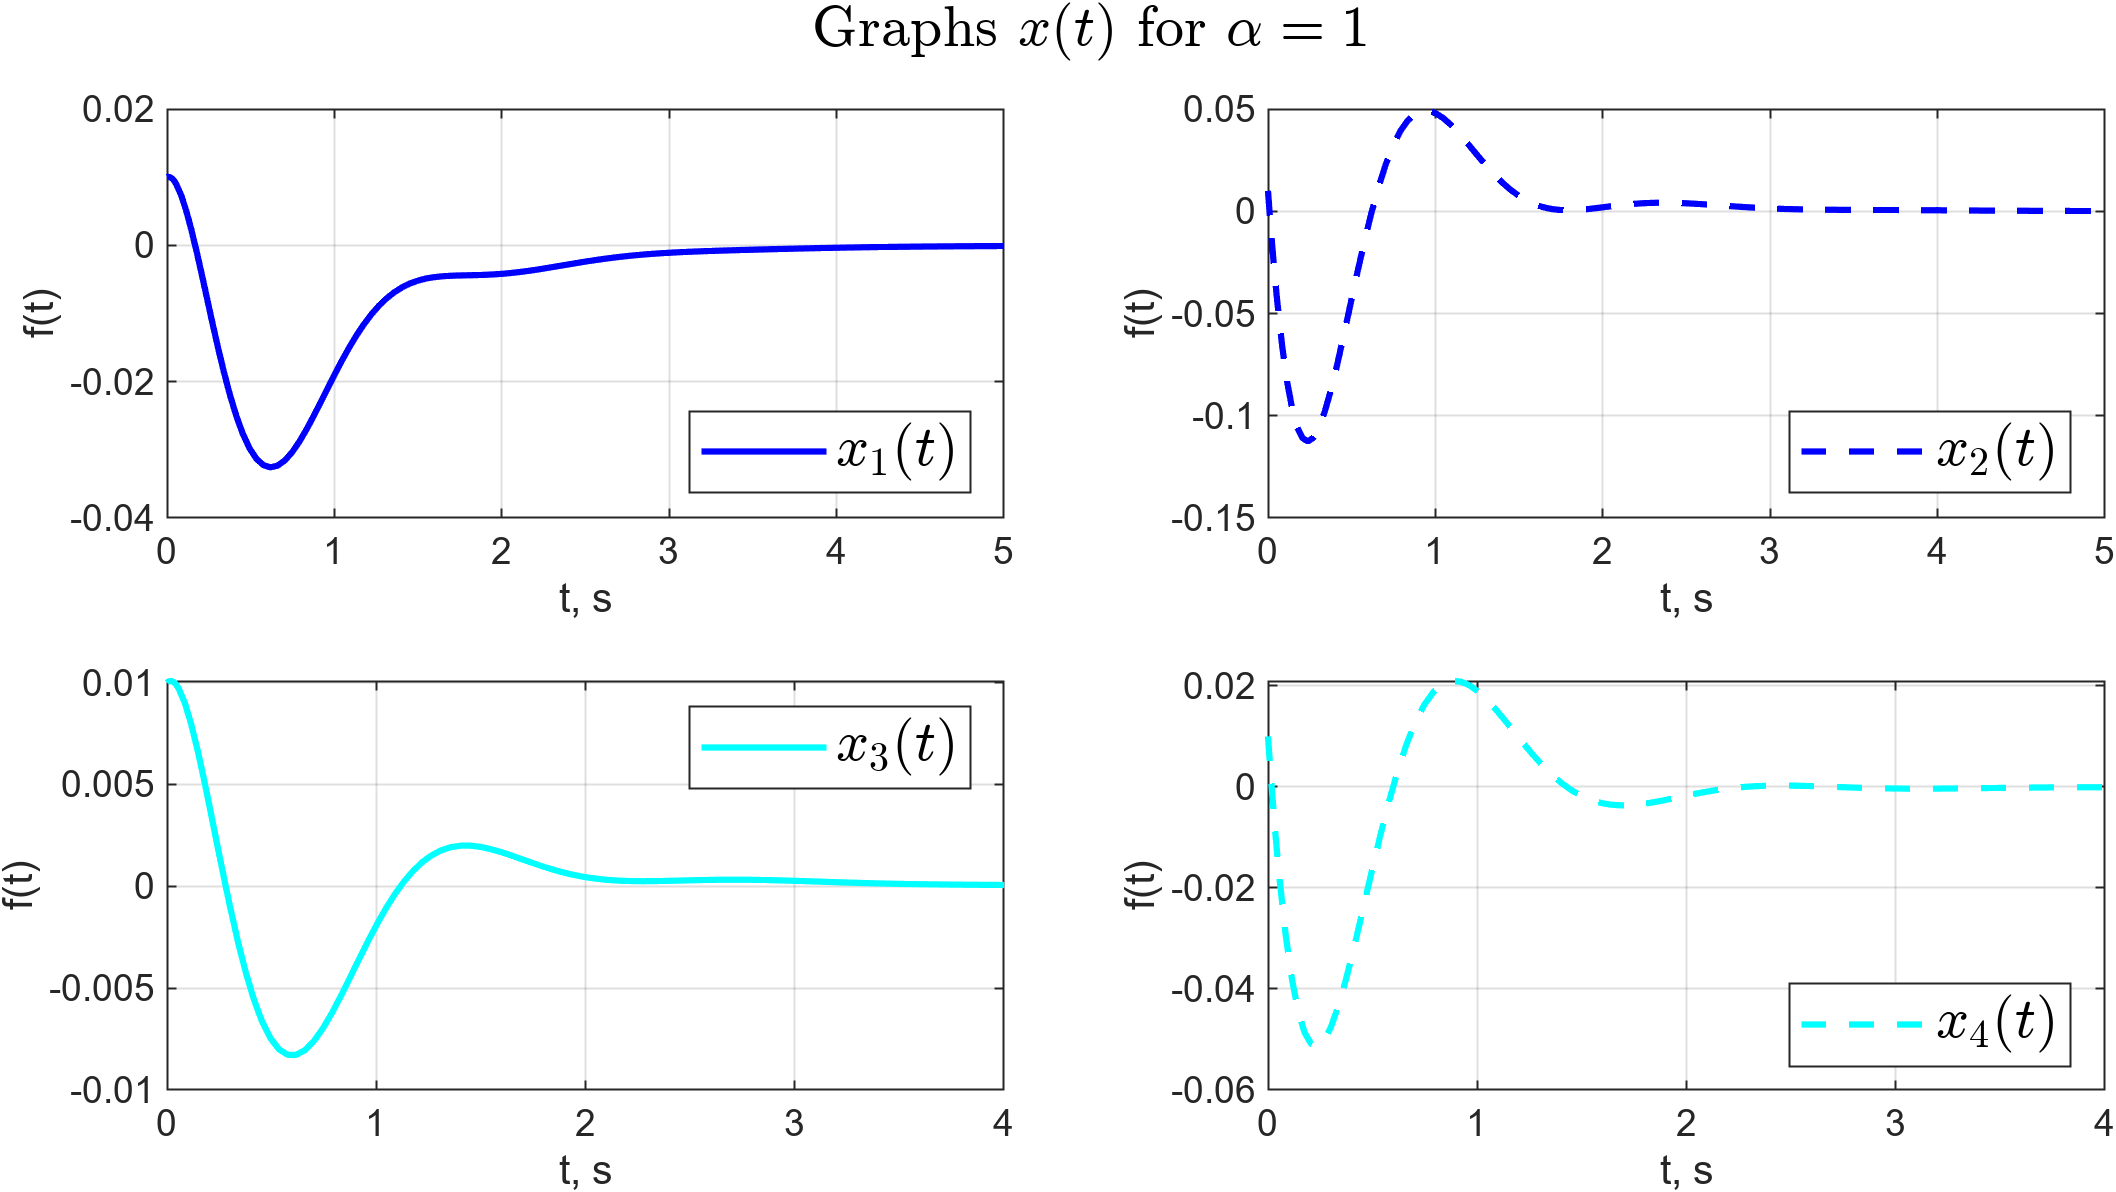
\includegraphics[width=1\linewidth]{pic_fix/4_2_x_1.png}}
	\caption{Графики вектора состояния системы при $\alpha = 1$.}
	\label{4_2_x_1}
\end{figure}

\begin{figure}[!h]
	\center{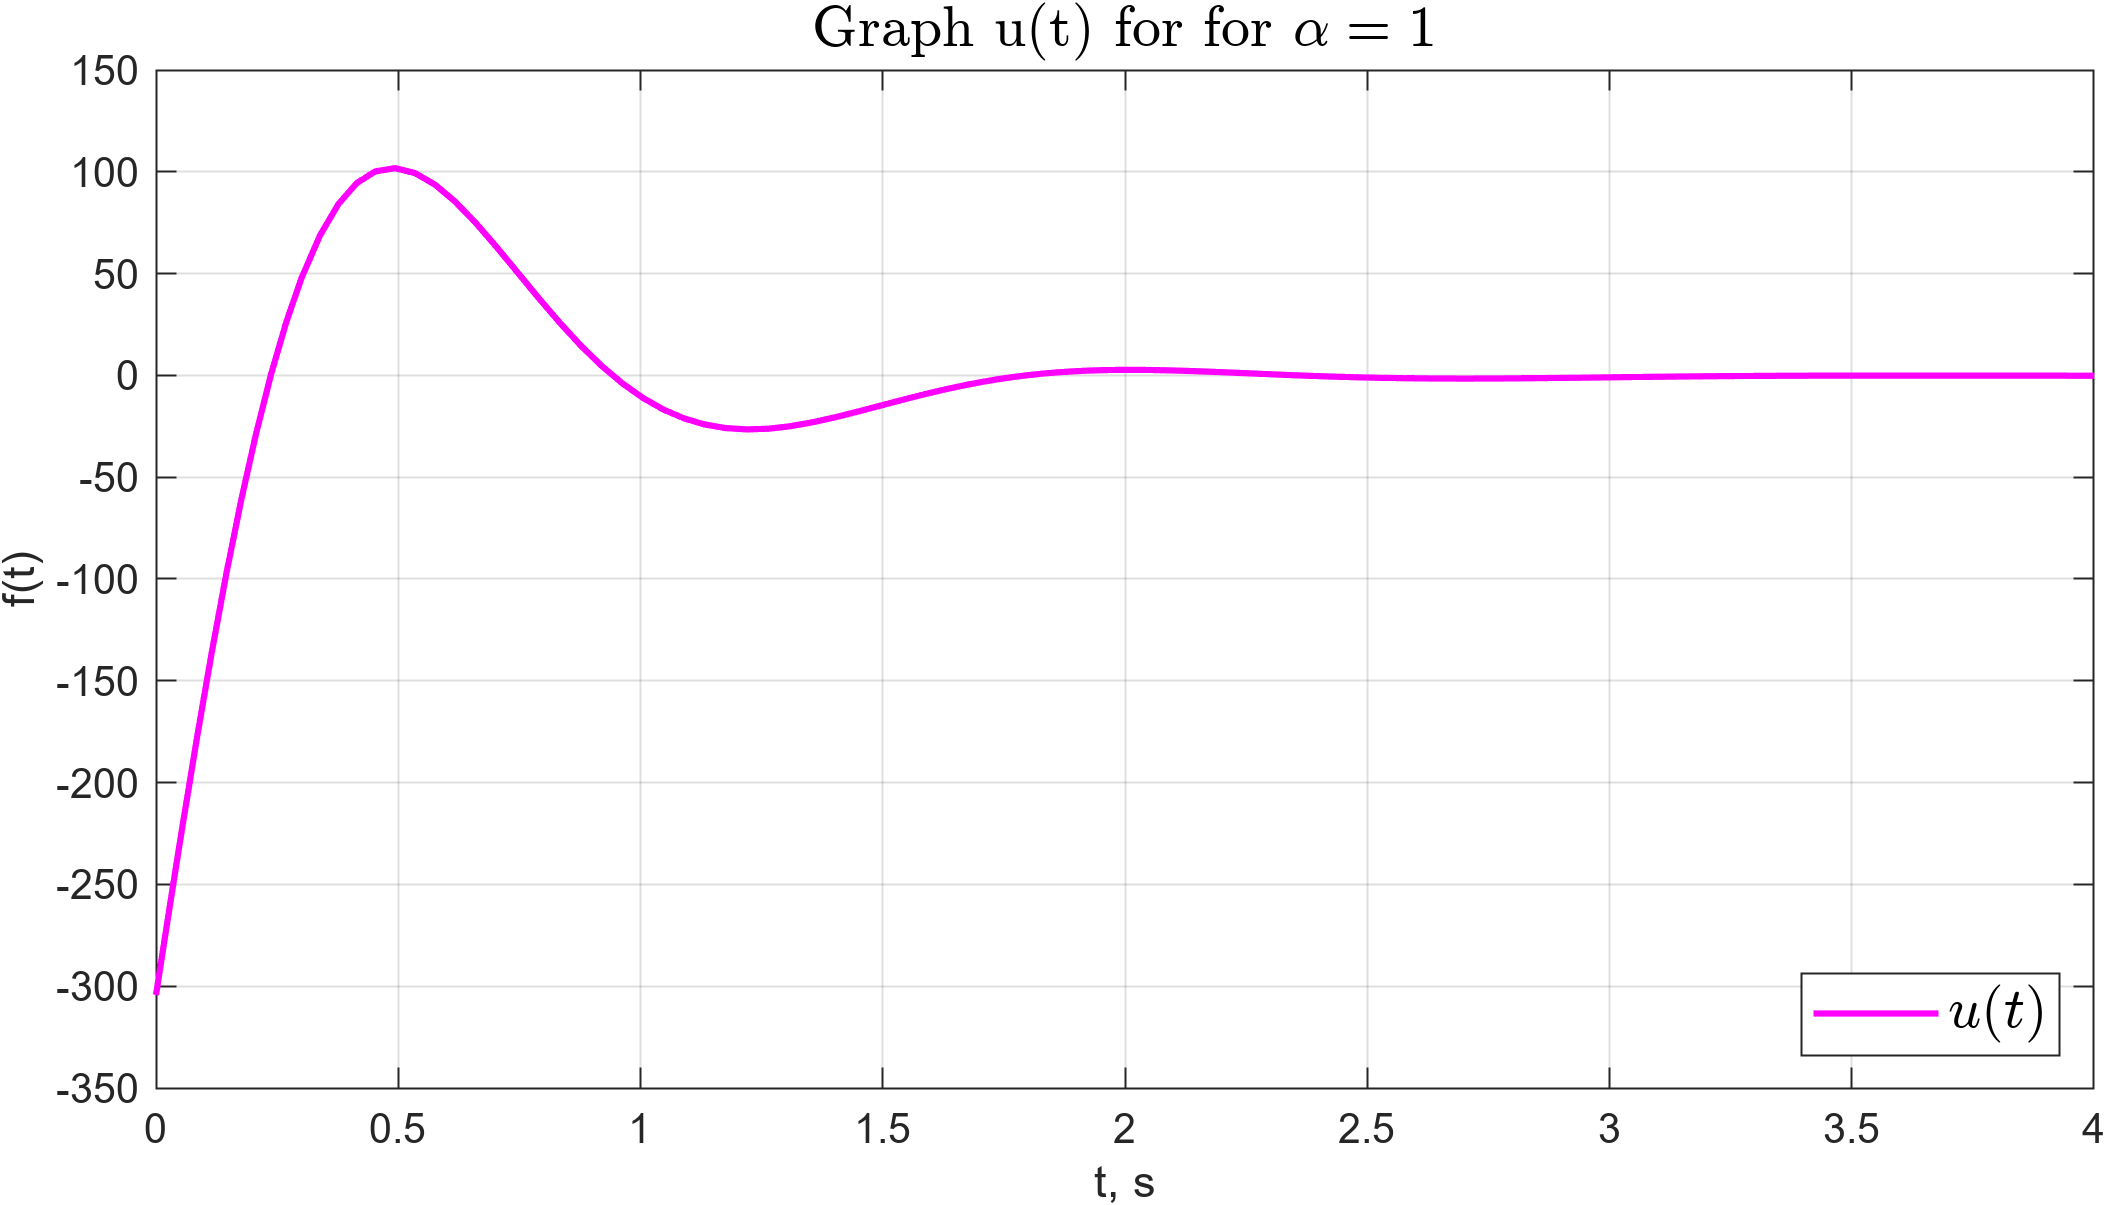
\includegraphics[width=1\linewidth]{pic_fix/4_2_u_1.png}}
	\caption{График $u(t)$ при $\alpha = 1$.}
	\label{4_2_u_1}
\end{figure}


\begin{figure}[!h]
	\center{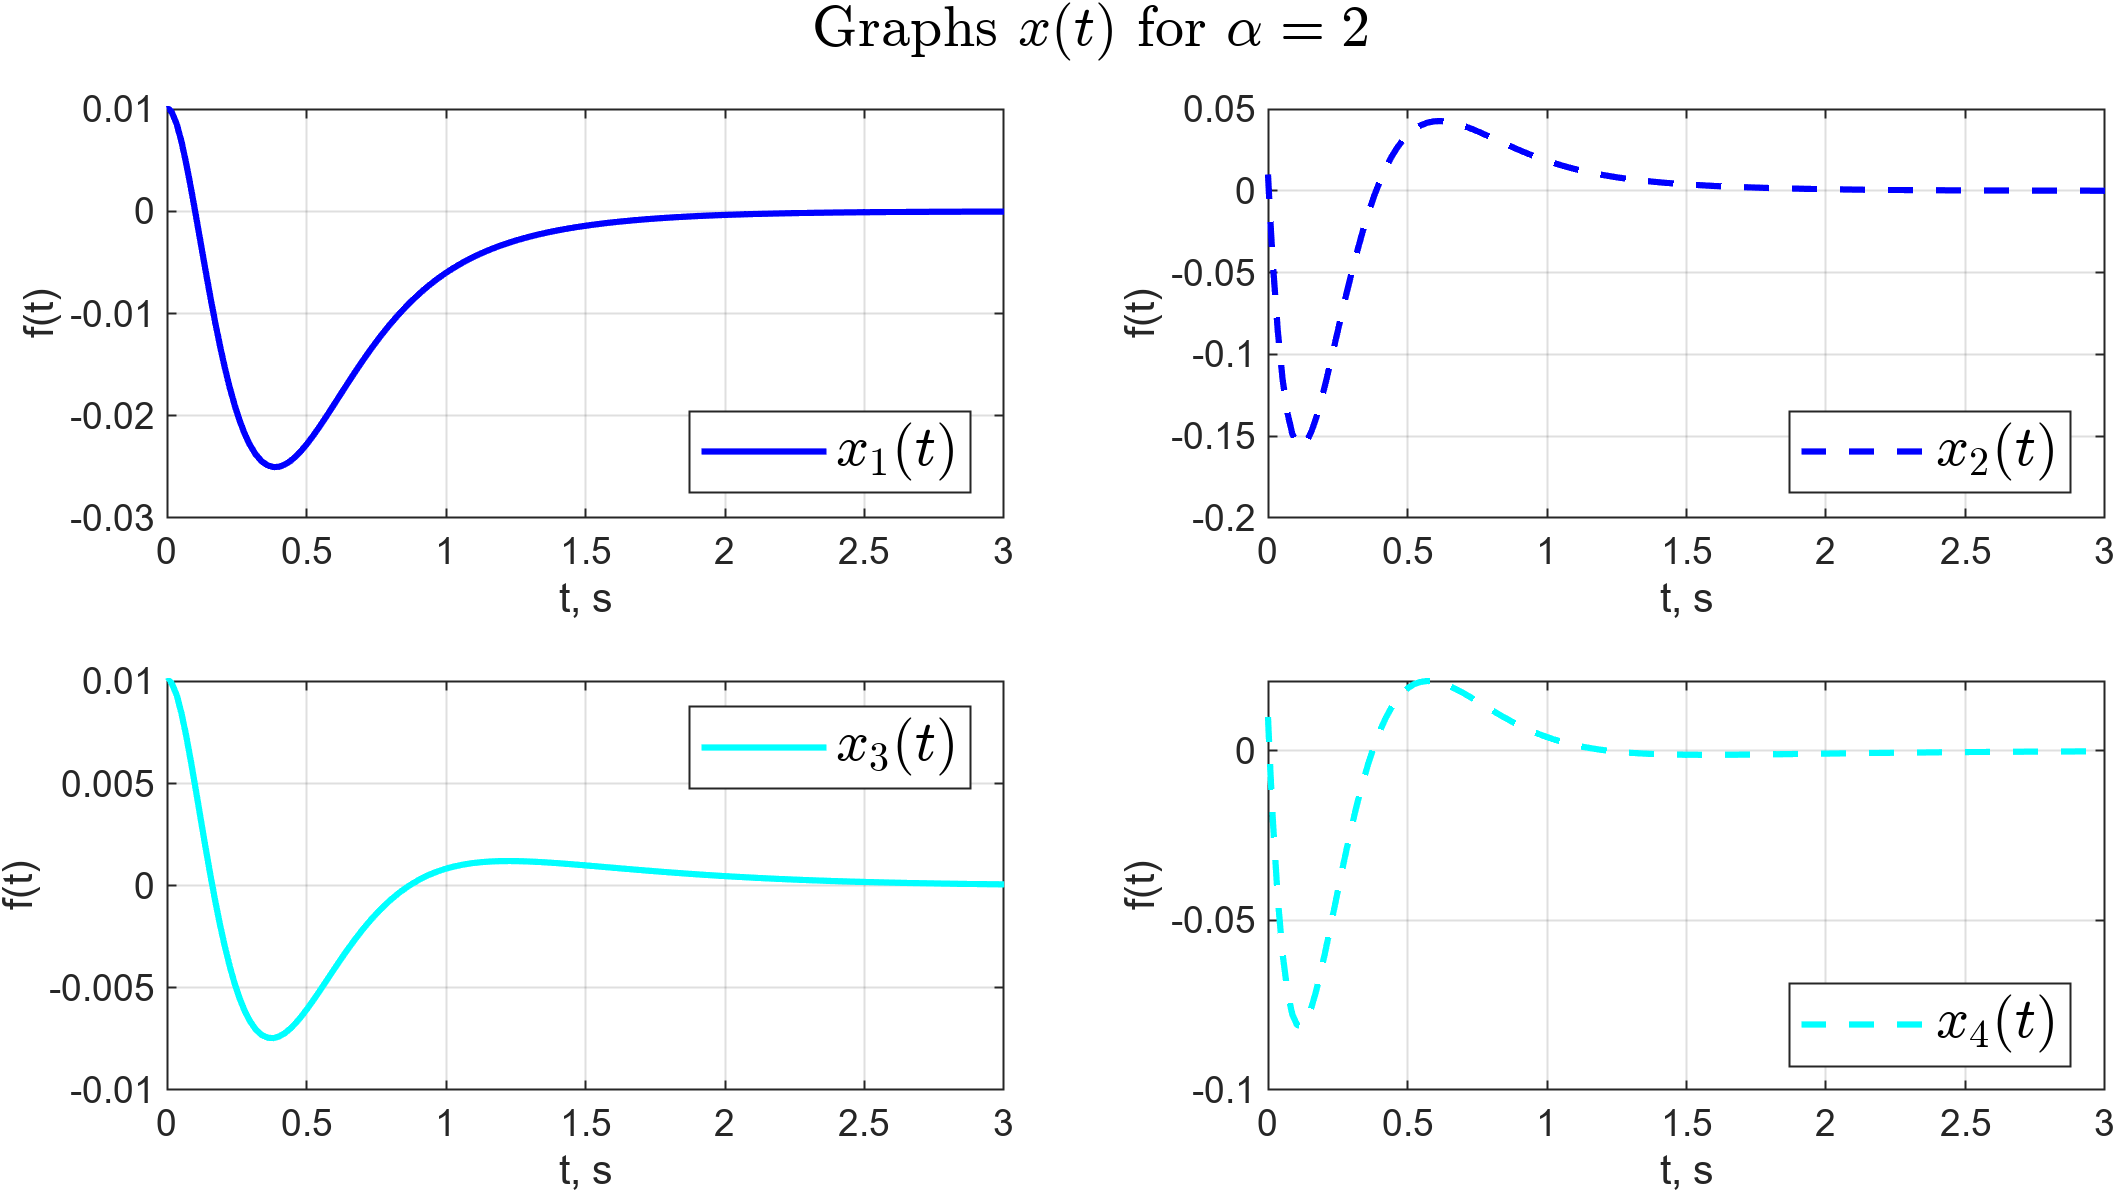
\includegraphics[width=1\linewidth]{pic_fix/4_2_x_2.png}}
	\caption{Графики вектора состояния системы при $\alpha = 2$.}
	\label{4_2_x_2}
\end{figure}

\begin{figure}[!h]
	\center{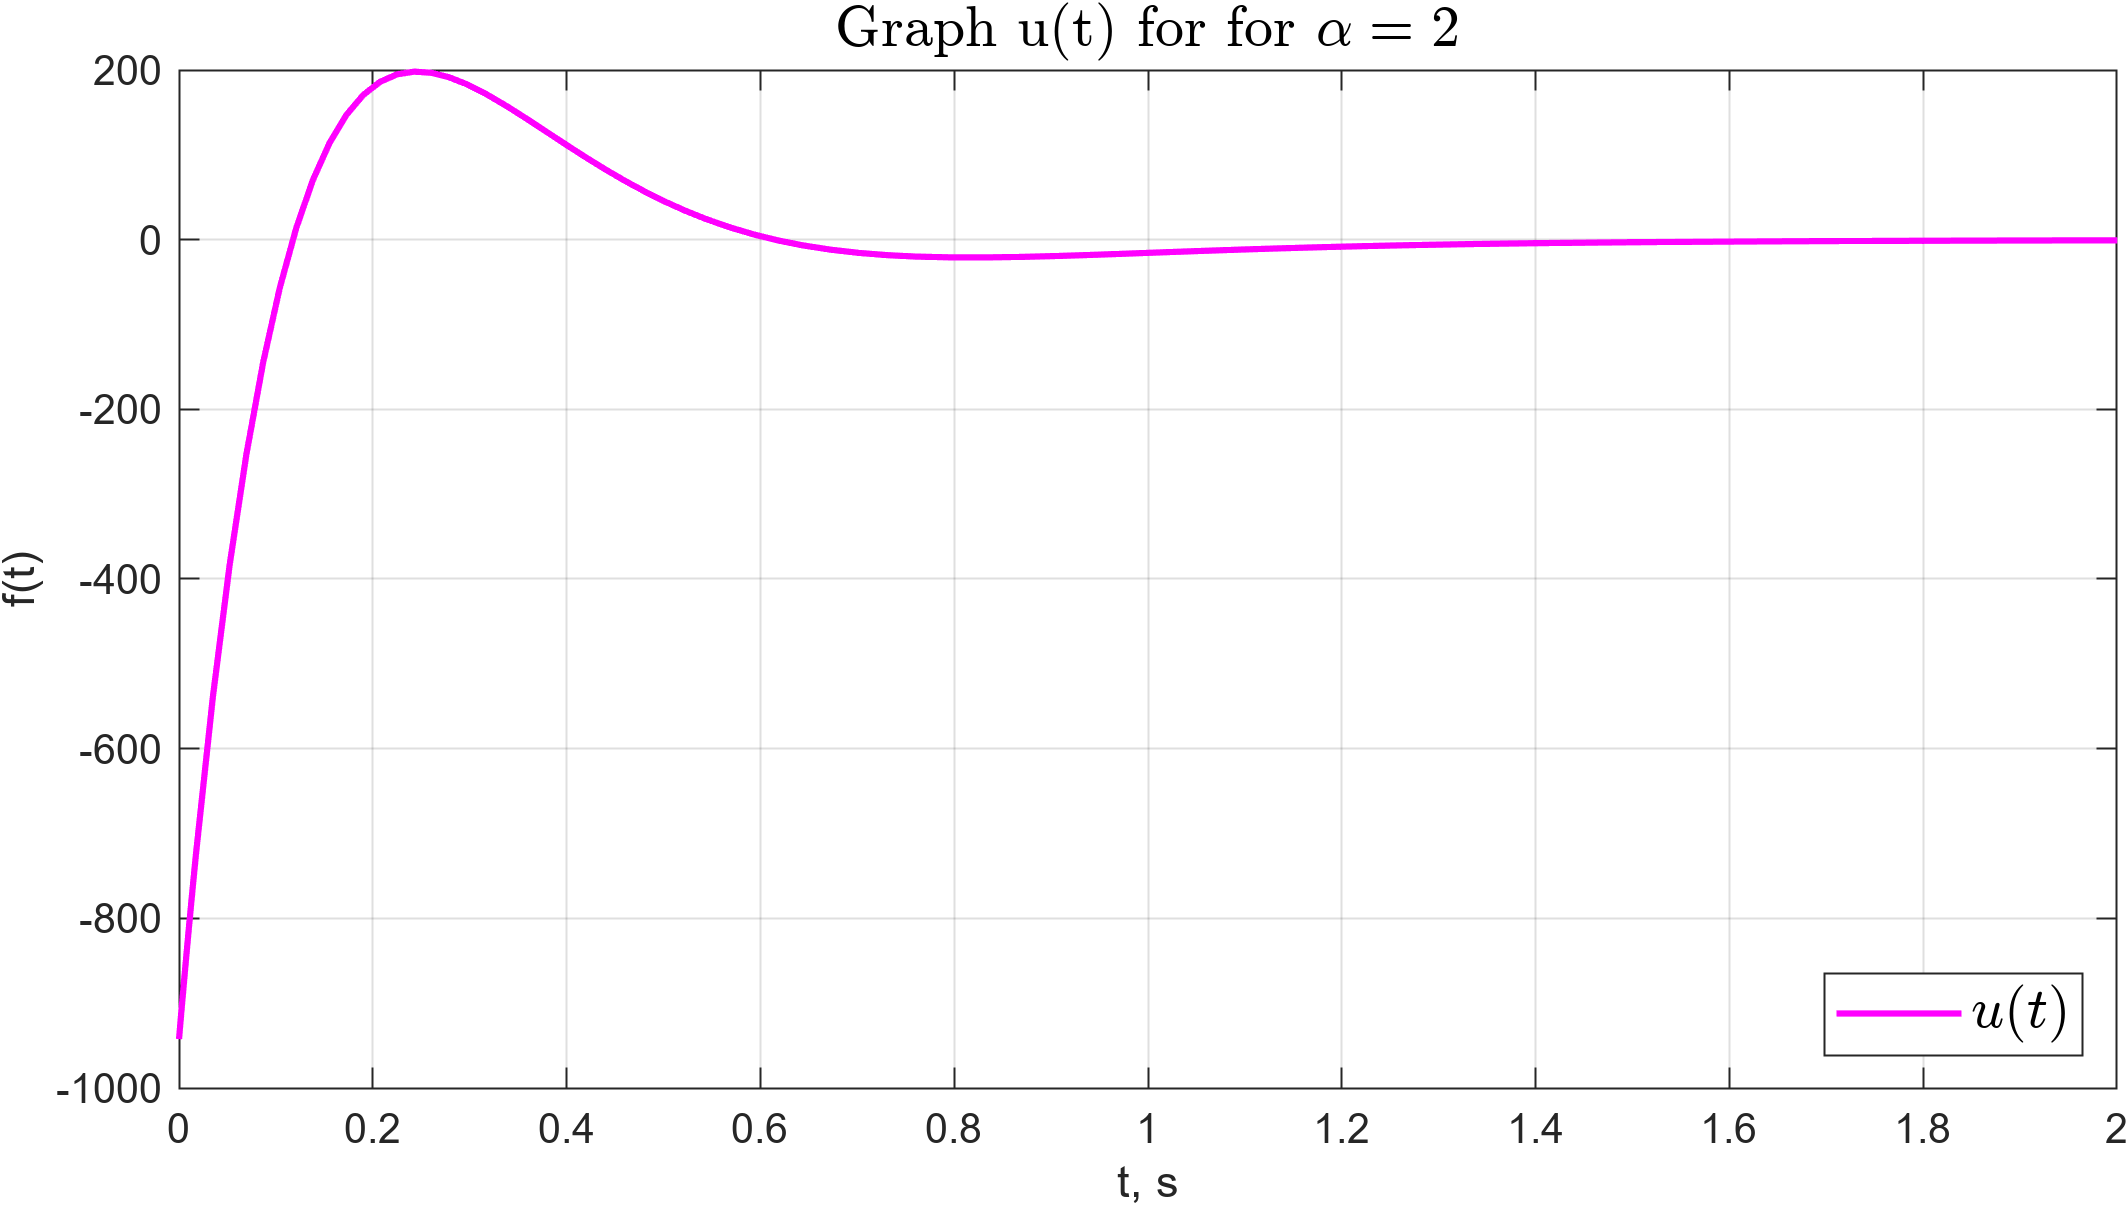
\includegraphics[width=1\linewidth]{pic_fix/4_2_u_2.png}}
	\caption{График $u(t)$ при $\alpha = 2$.}
	\label{4_2_u_2}
\end{figure}




\begin{figure}[!h]
	\center{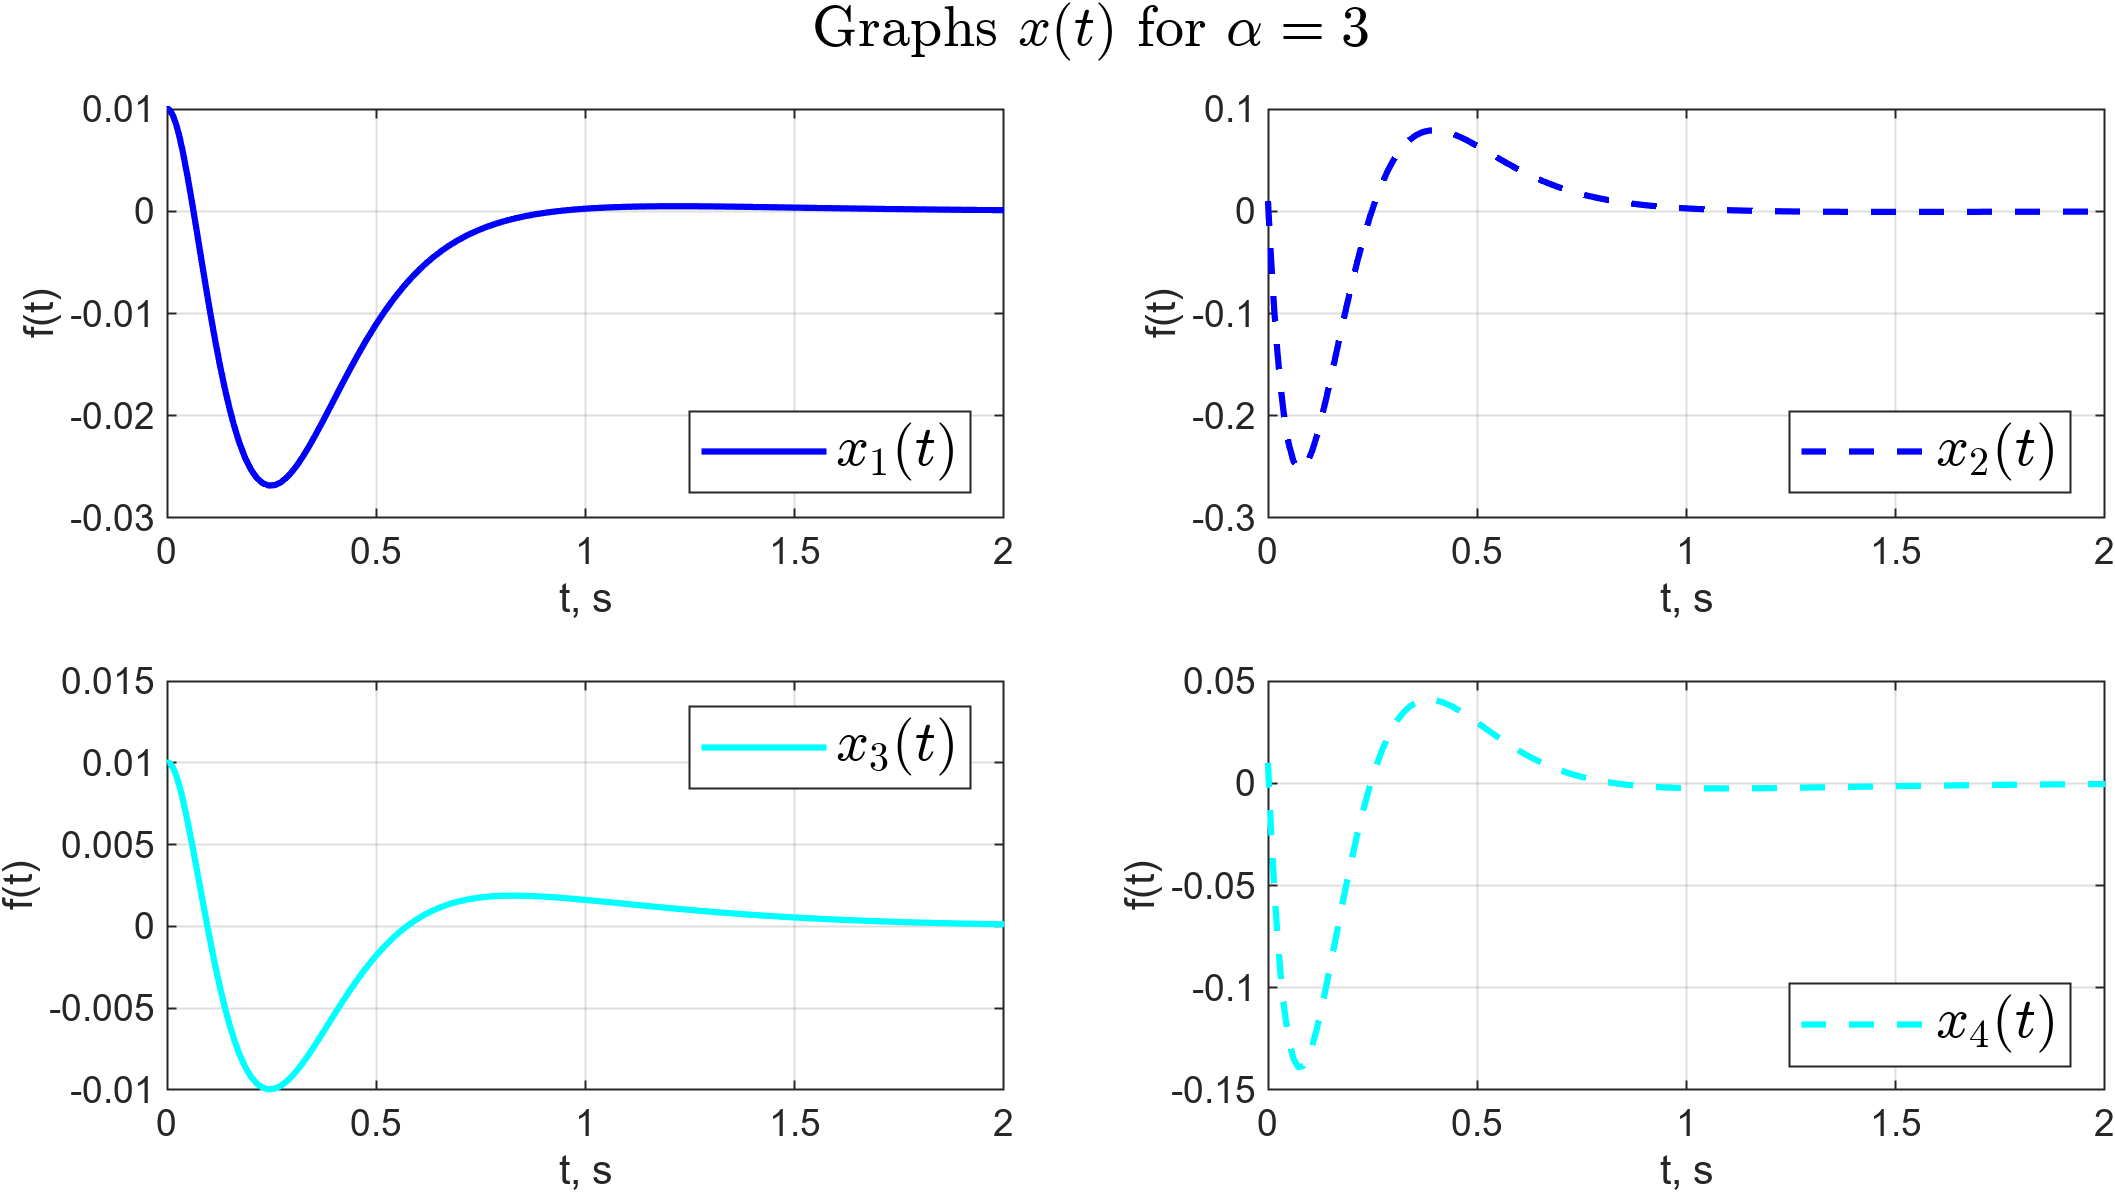
\includegraphics[width=1\linewidth]{pic_fix/4_2_x_3.png}}
	\caption{Графики вектора состояния системы при $\alpha = 3$.}
	\label{4_2_x_3}
\end{figure}

\begin{figure}[!h]
	\center{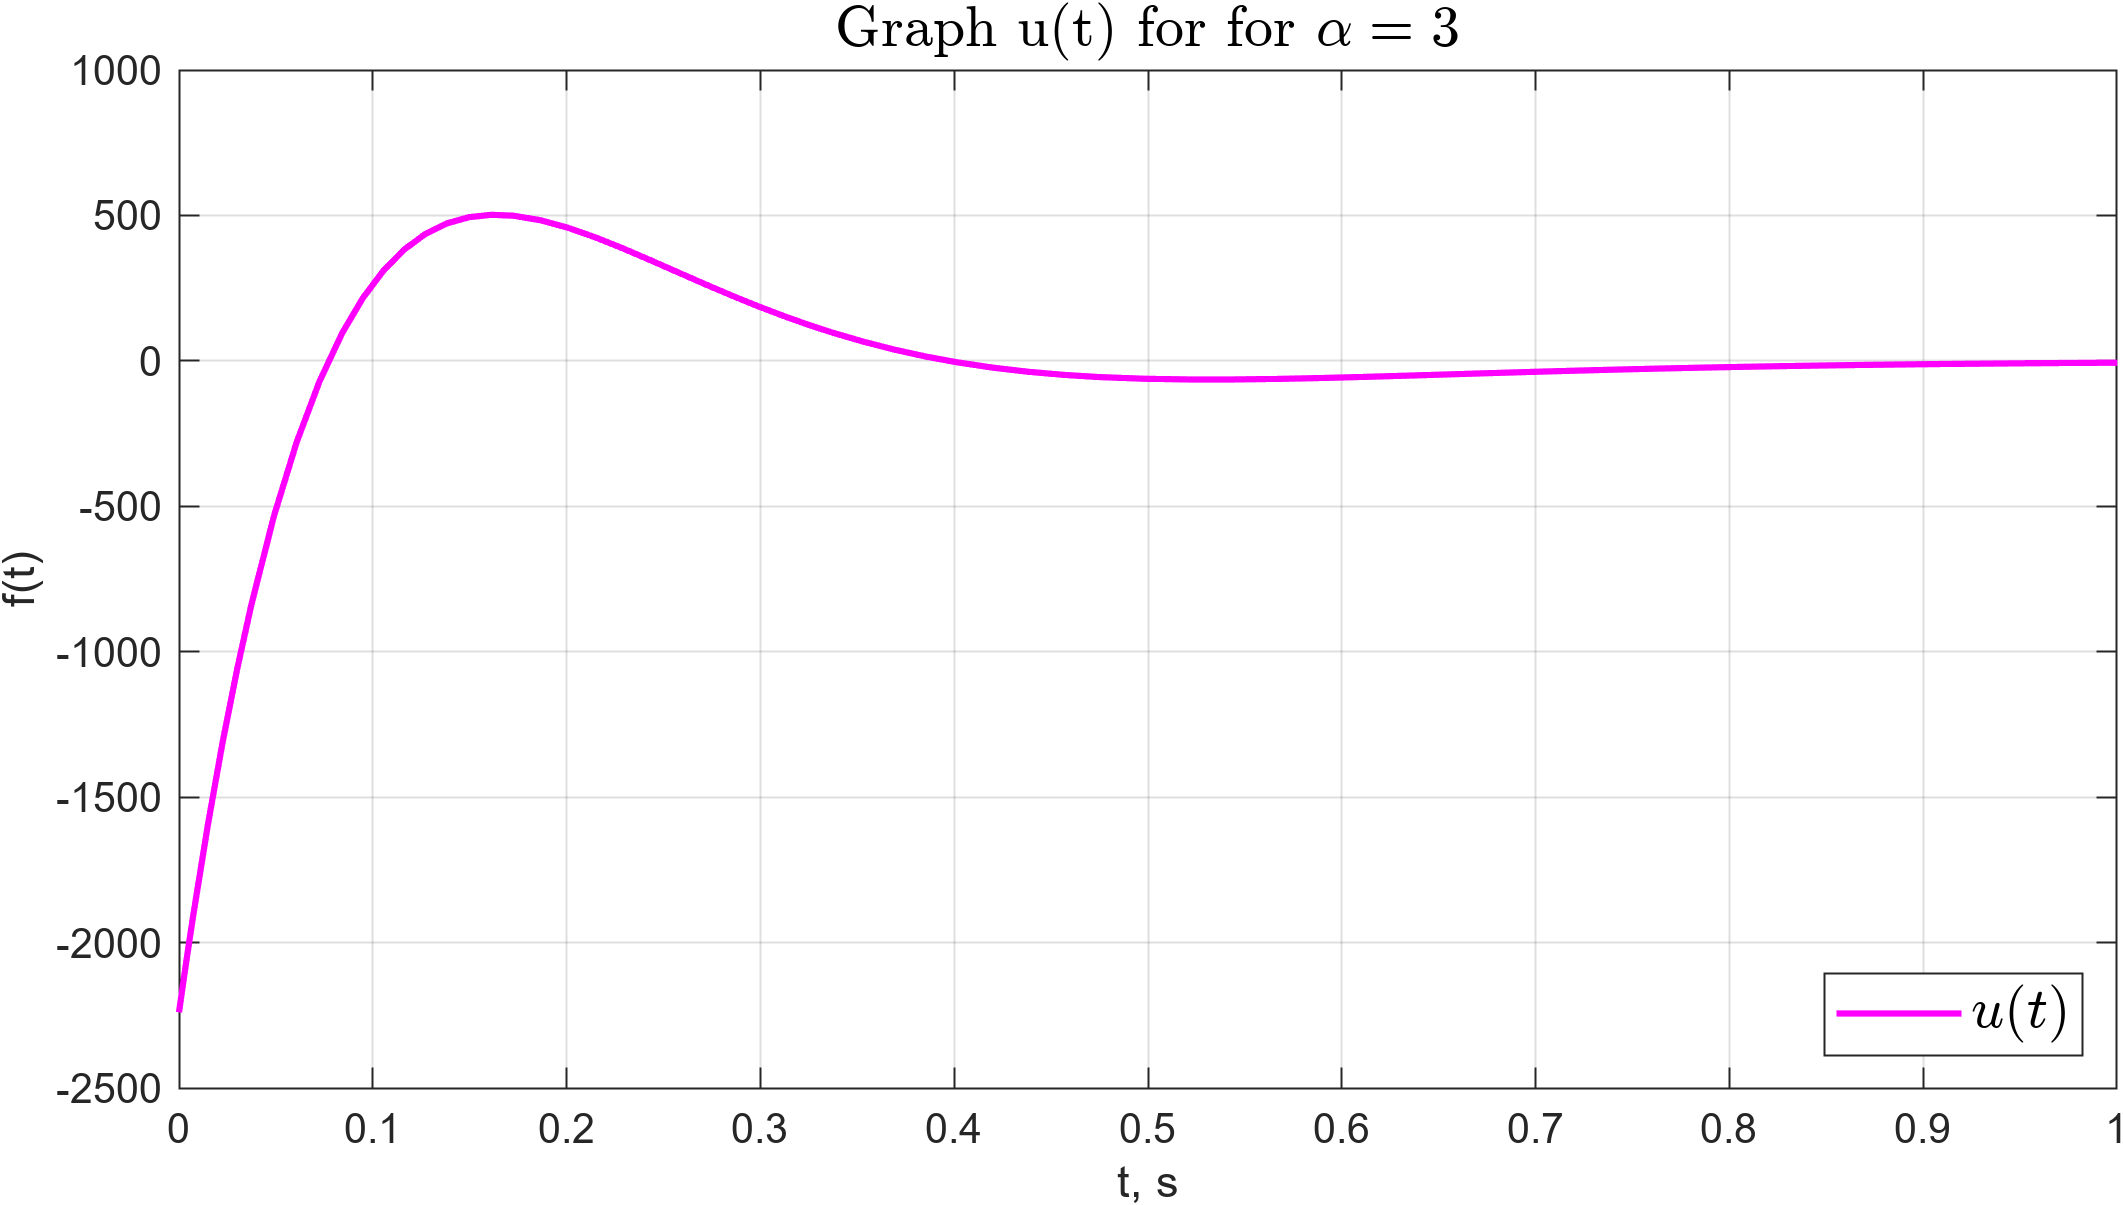
\includegraphics[width=1\linewidth]{pic_fix/4_2_u_3.png}}
	\caption{График $u(t)$ при $\alpha = 3$.}
	\label{4_2_u_3}
\end{figure}


\begin{figure}[!h]
	\center{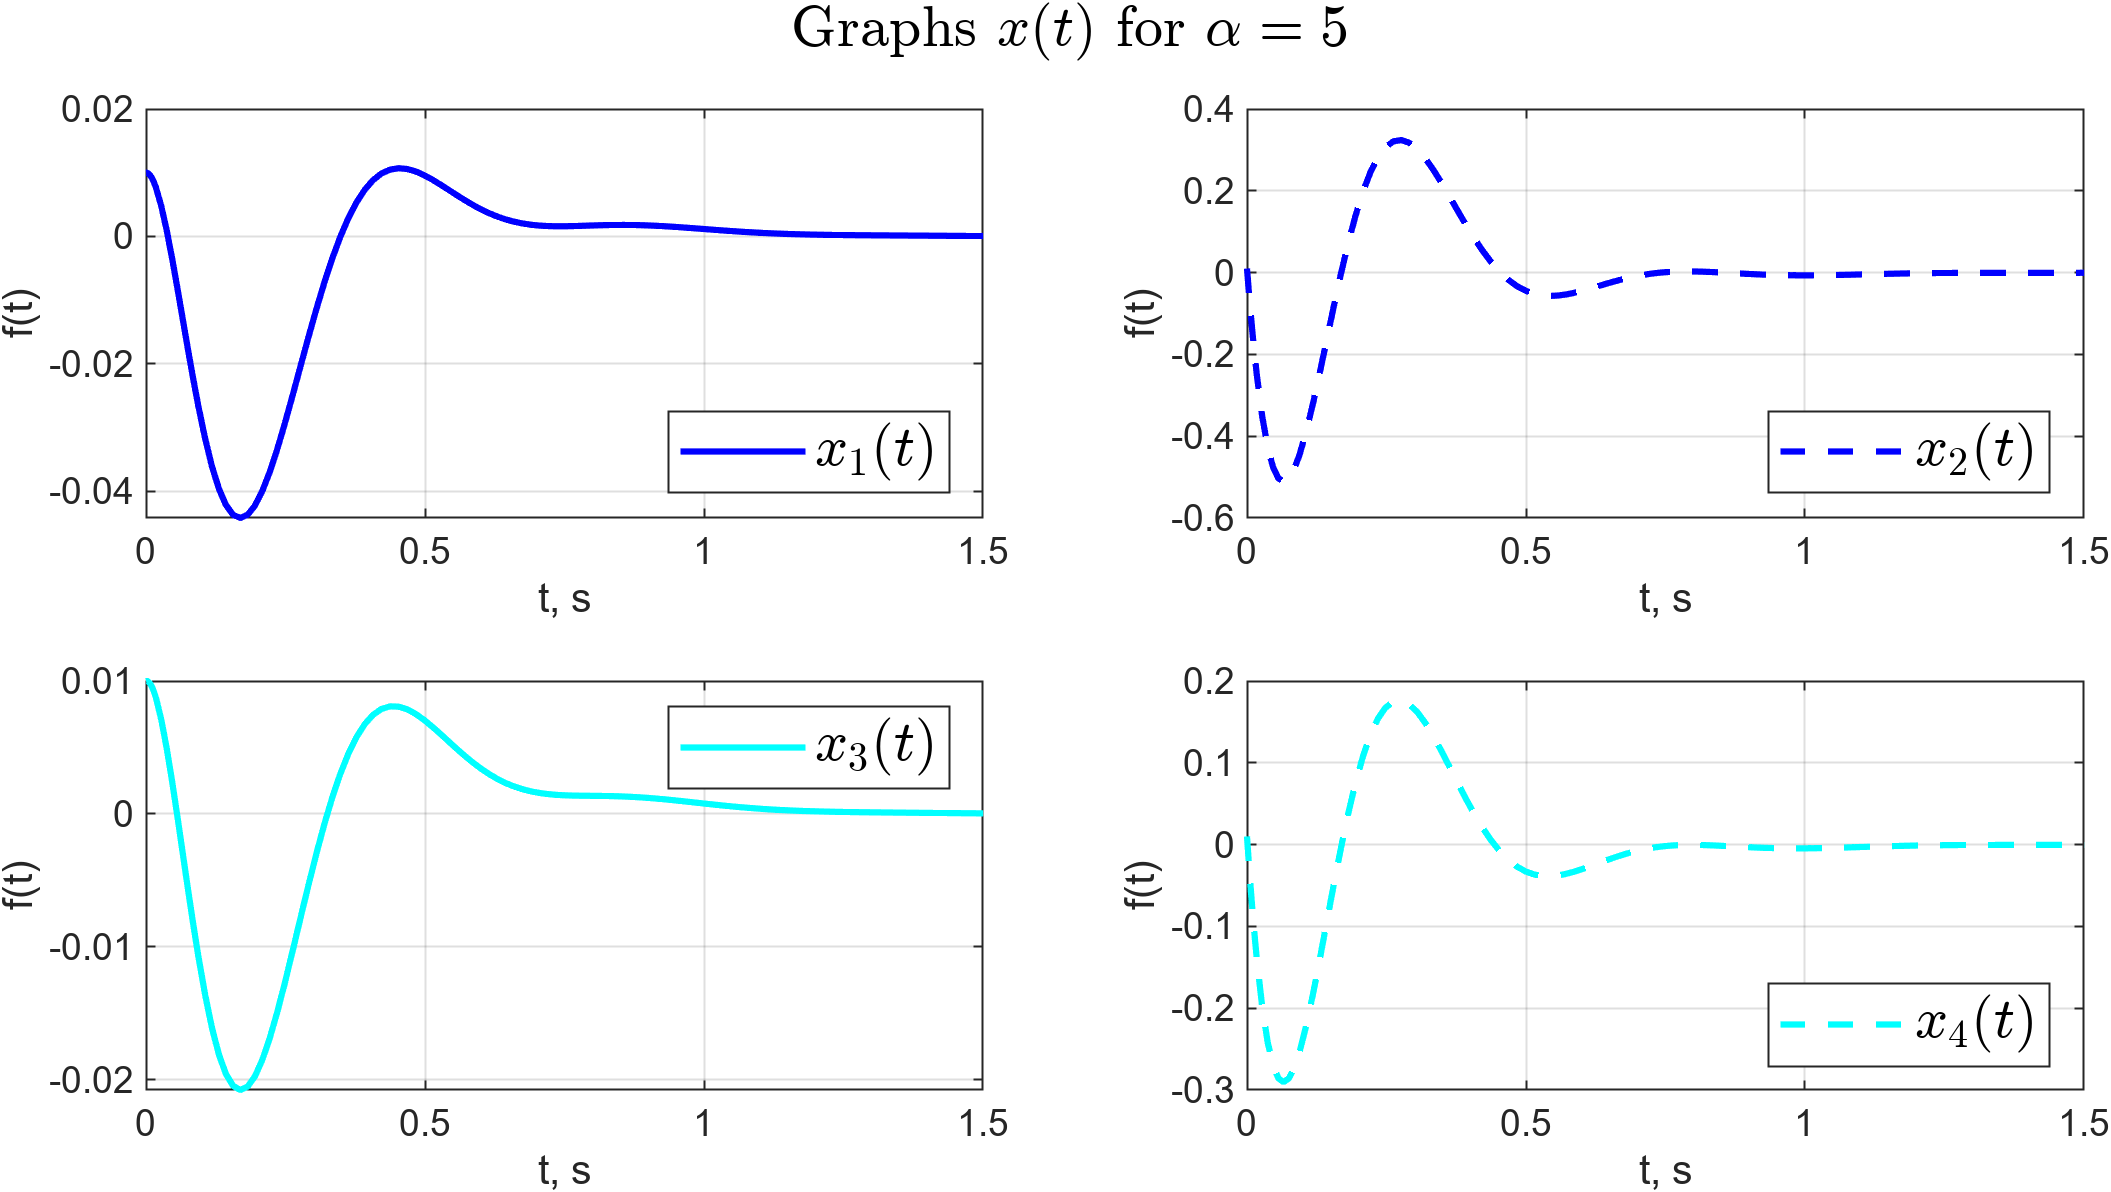
\includegraphics[width=1\linewidth]{pic_fix/4_2_x_5.png}}
	\caption{Графики вектора состояния системы при $\alpha = 5$.}
	\label{4_2_x_5}
\end{figure}

\begin{figure}[!h]
	\center{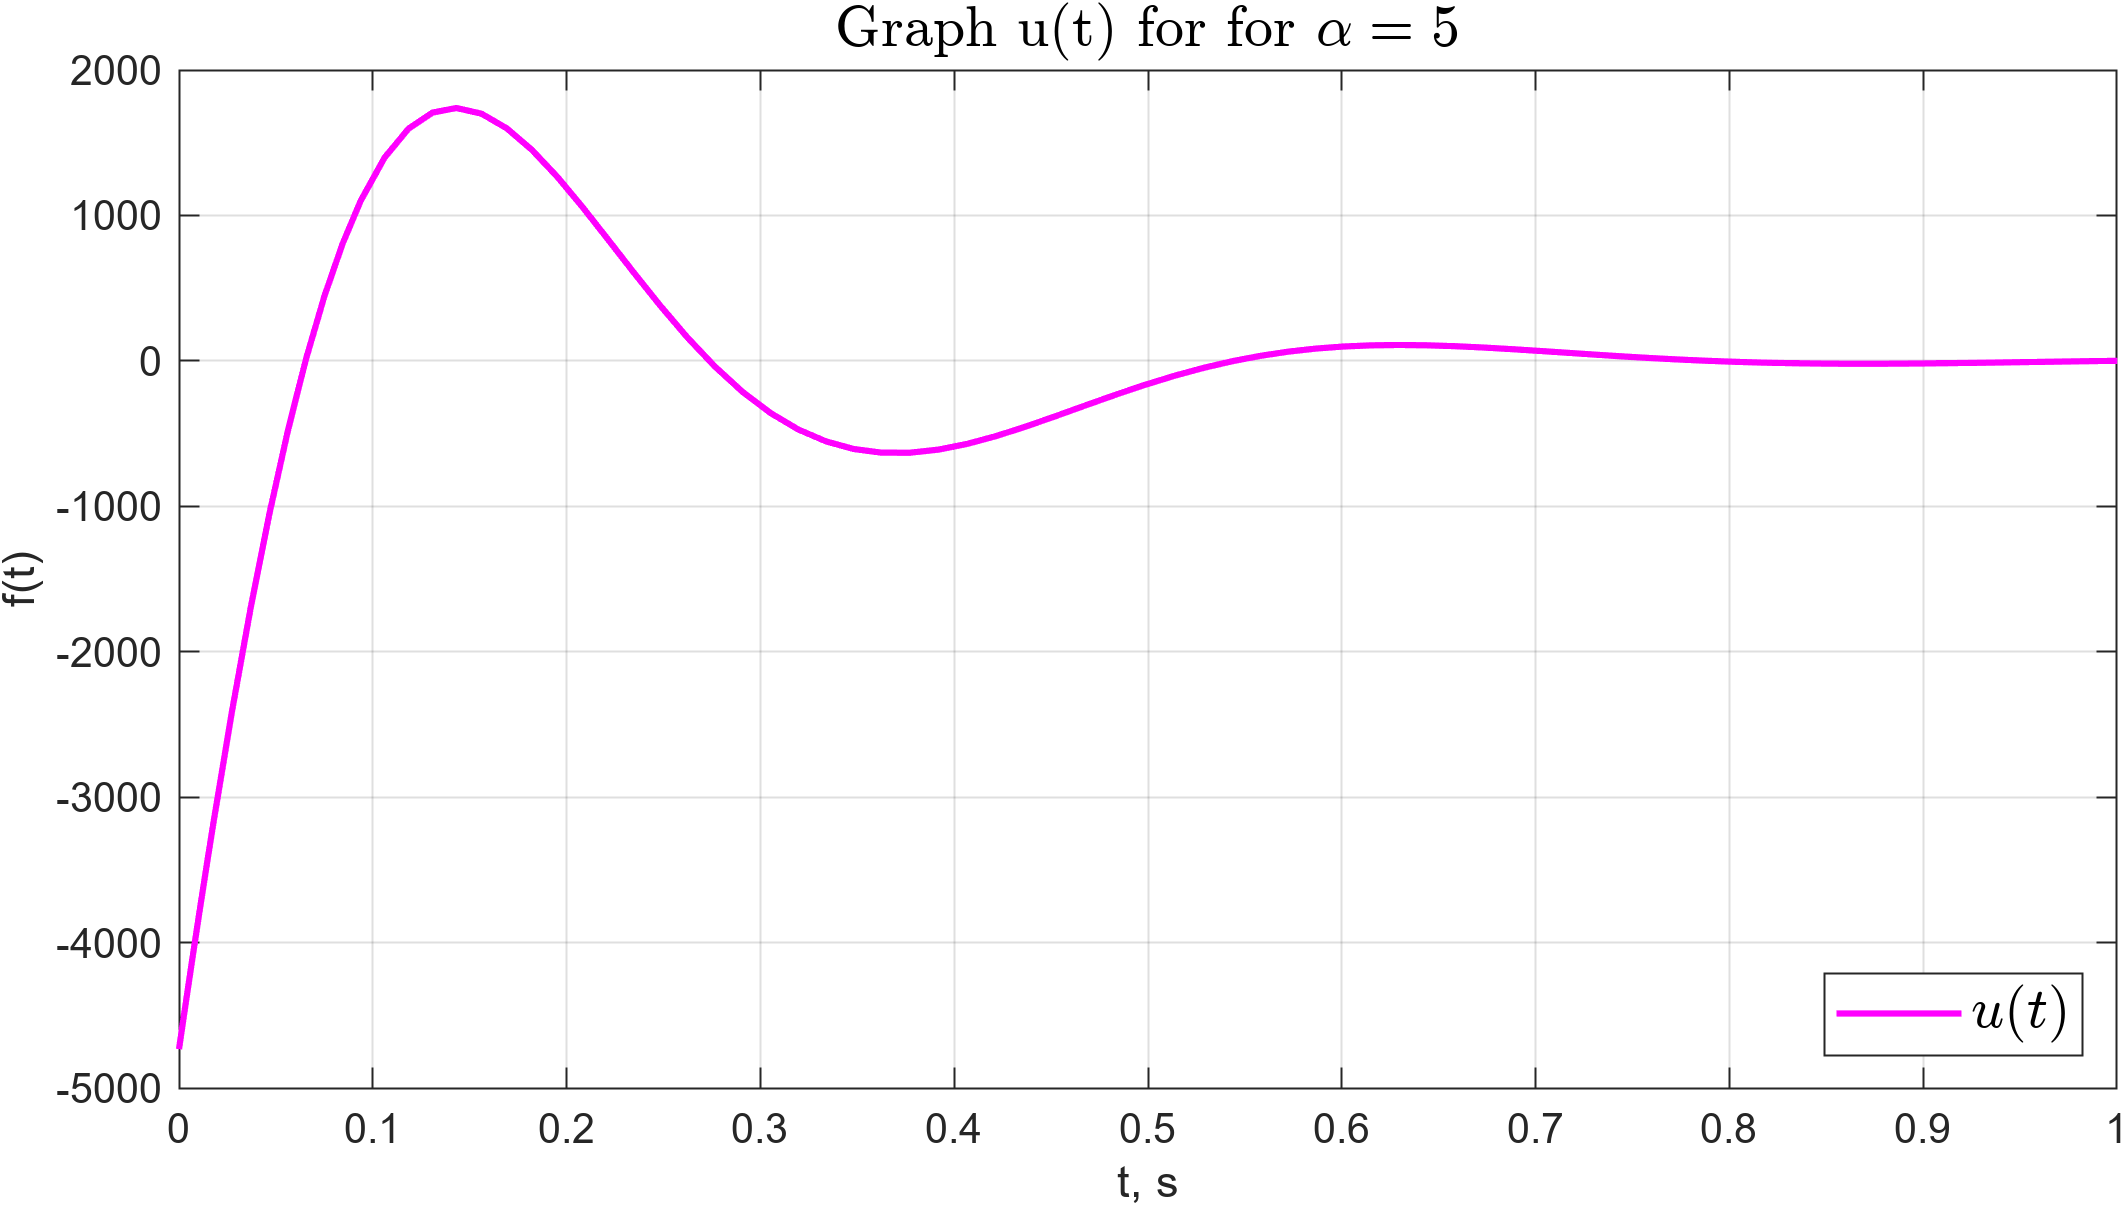
\includegraphics[width=1\linewidth]{pic_fix/4_2_u_5.png}}
	\caption{График $u(t)$ при $\alpha = 5$.}
	\label{4_2_u_5}
\end{figure}



\begin{figure}[!h]
	\center{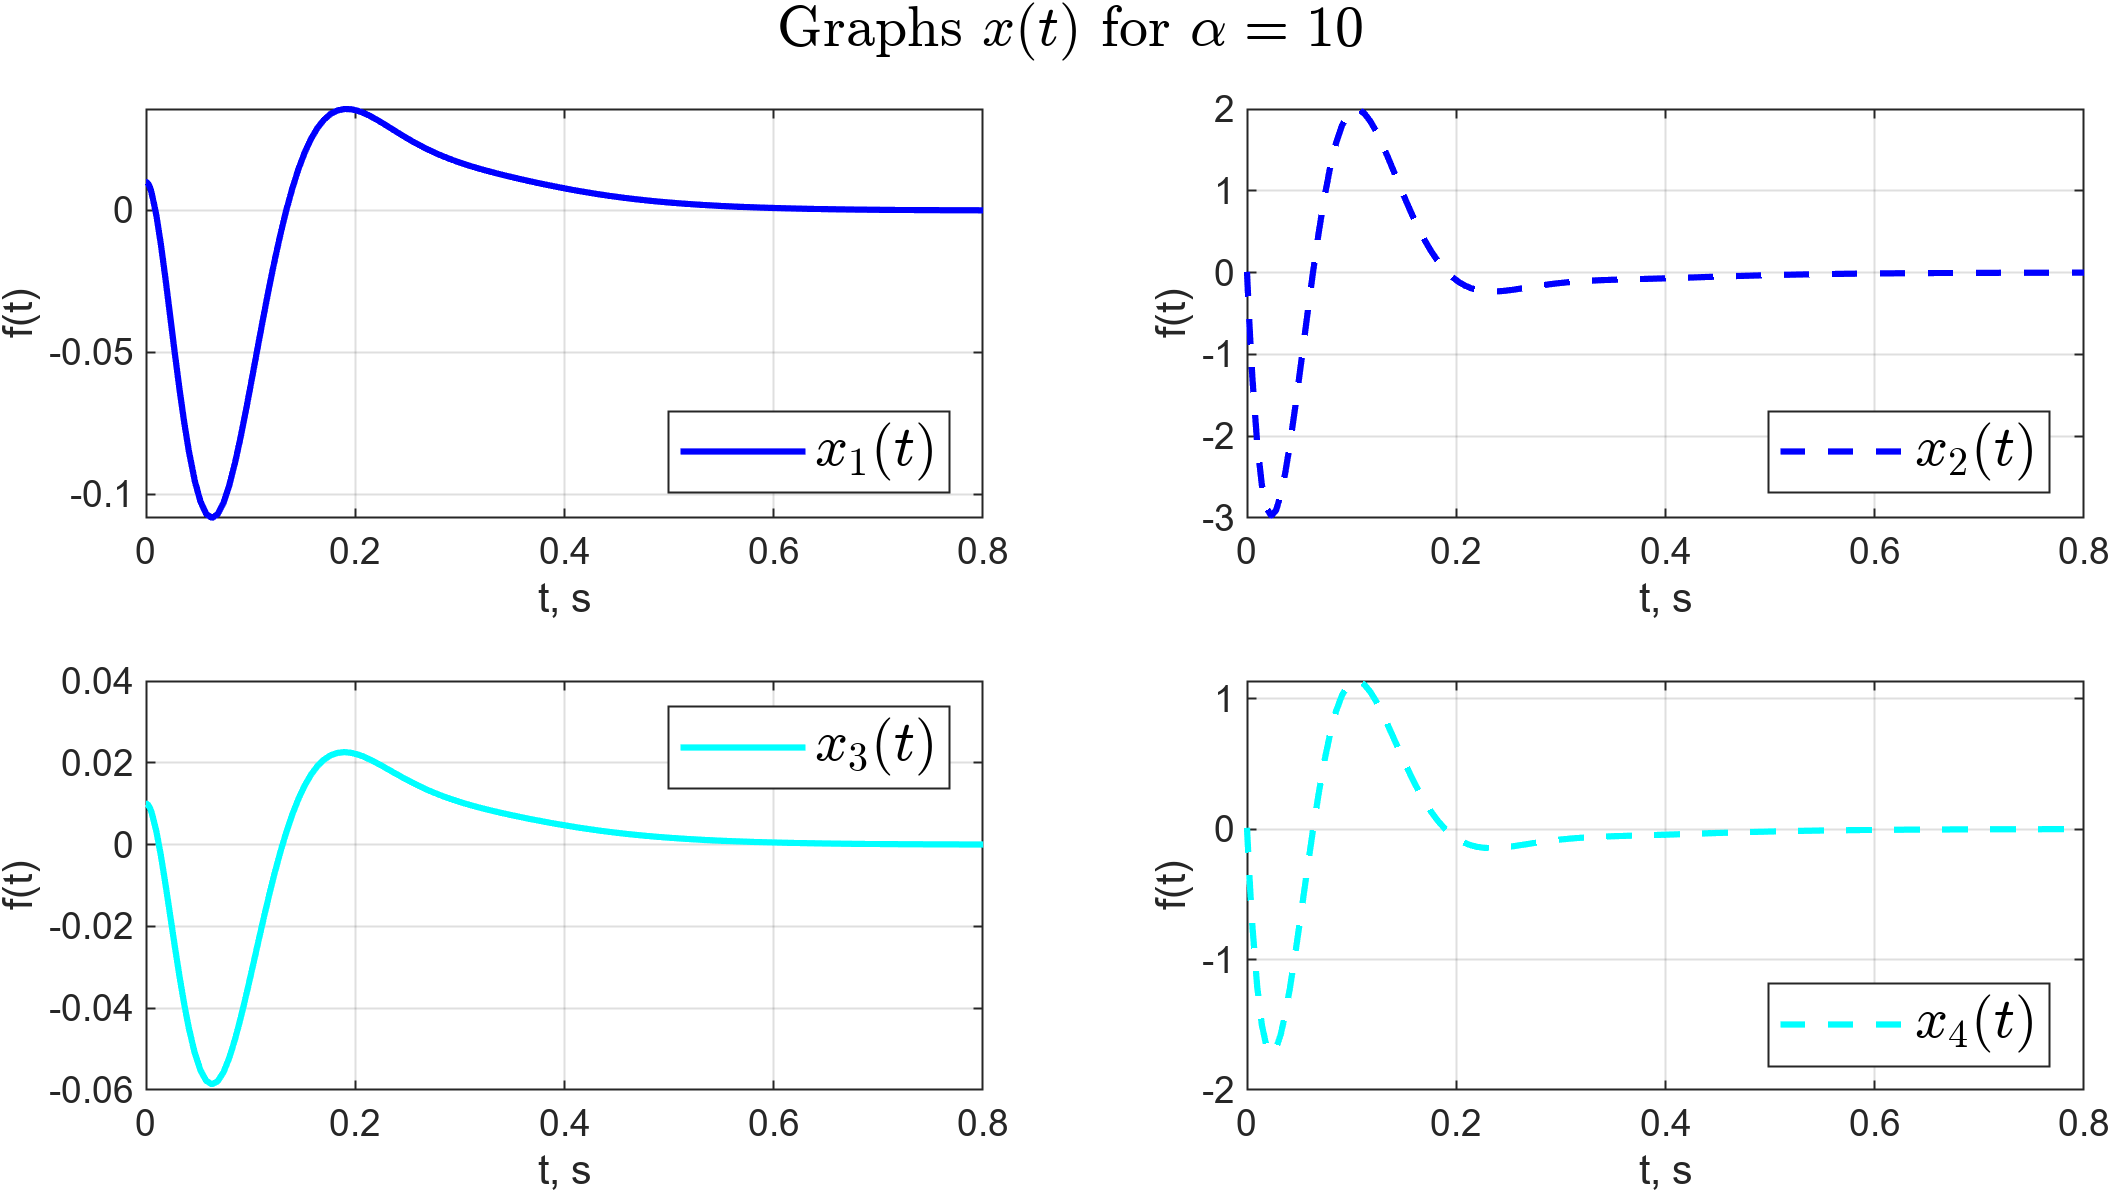
\includegraphics[width=1\linewidth]{pic_fix/4_2_x_10.png}}
	\caption{Графики вектора состояния системы при $\alpha = 10$.}
	\label{4_2_x_10}
\end{figure}

\begin{figure}[!h]
	\center{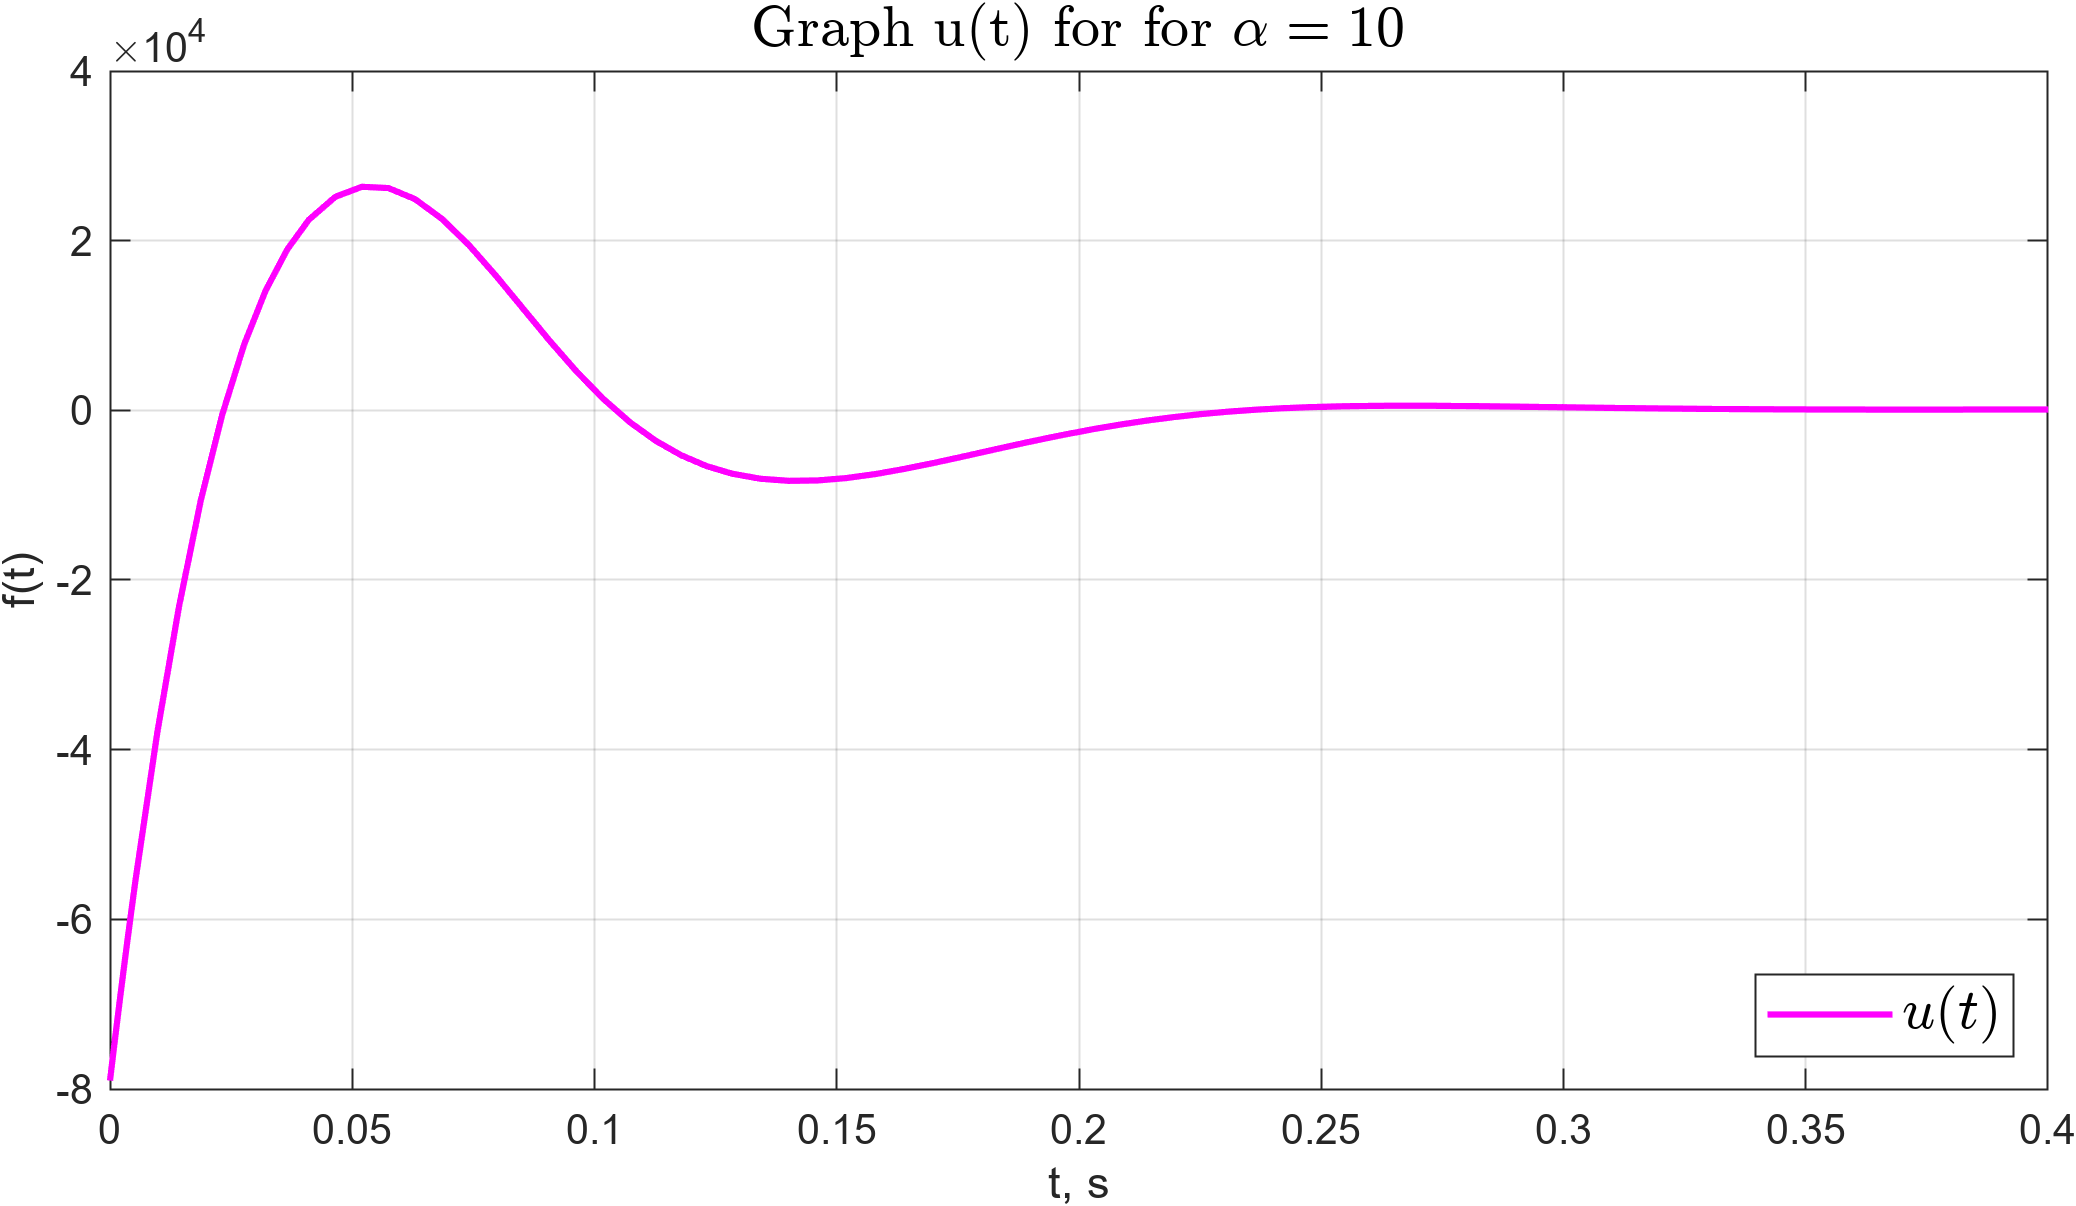
\includegraphics[width=1\linewidth]{pic_fix/4_2_u_10.png}}
	\caption{График $u(t)$ при $\alpha = 10$.}
	\label{4_2_u_10}
\end{figure}


\section{Синтез регулятора по состоянию с ограничением на управление}

Зададимся следующими значениями параметра: $\alpha_1= 0.1$, $\alpha_2 = 0.5$, $\alpha_3 = 1$ и выполним расчет регулятора $u=Kx$ такого, чтобы наибольшее значение модуля управляющего сигнала $u$ было наименьшим из возможных, то есть при вычислении матрицы $K$ будем также решать задачу минимизации управления

\begin{equation}
    \begin{cases}
      PA^T+AP+2 \alpha P + Y^T B^T+BY \preceq 0,\\
        K = Y P^{-1}\\
        P \succ 0\\
        \begin{bmatrix}
            P & Y^T\\
            Y & \gamma
        \end{bmatrix} \succ 0\\[2pt]
        \begin{bmatrix}
            P & x(0)\\
            x^T(0) & 1
        \end{bmatrix} \succ 0
    \end{cases},
\end{equation}

Для $\alpha_1=0.1$ матрица регулятора (моделирование -- рисунок \ref{4_3_1})

\begin{equation}
    K = \begin{bmatrix}
        4.5 & 49 & -3219 & -1334
    \end{bmatrix}
\end{equation}

\begin{figure}[!h]
\center{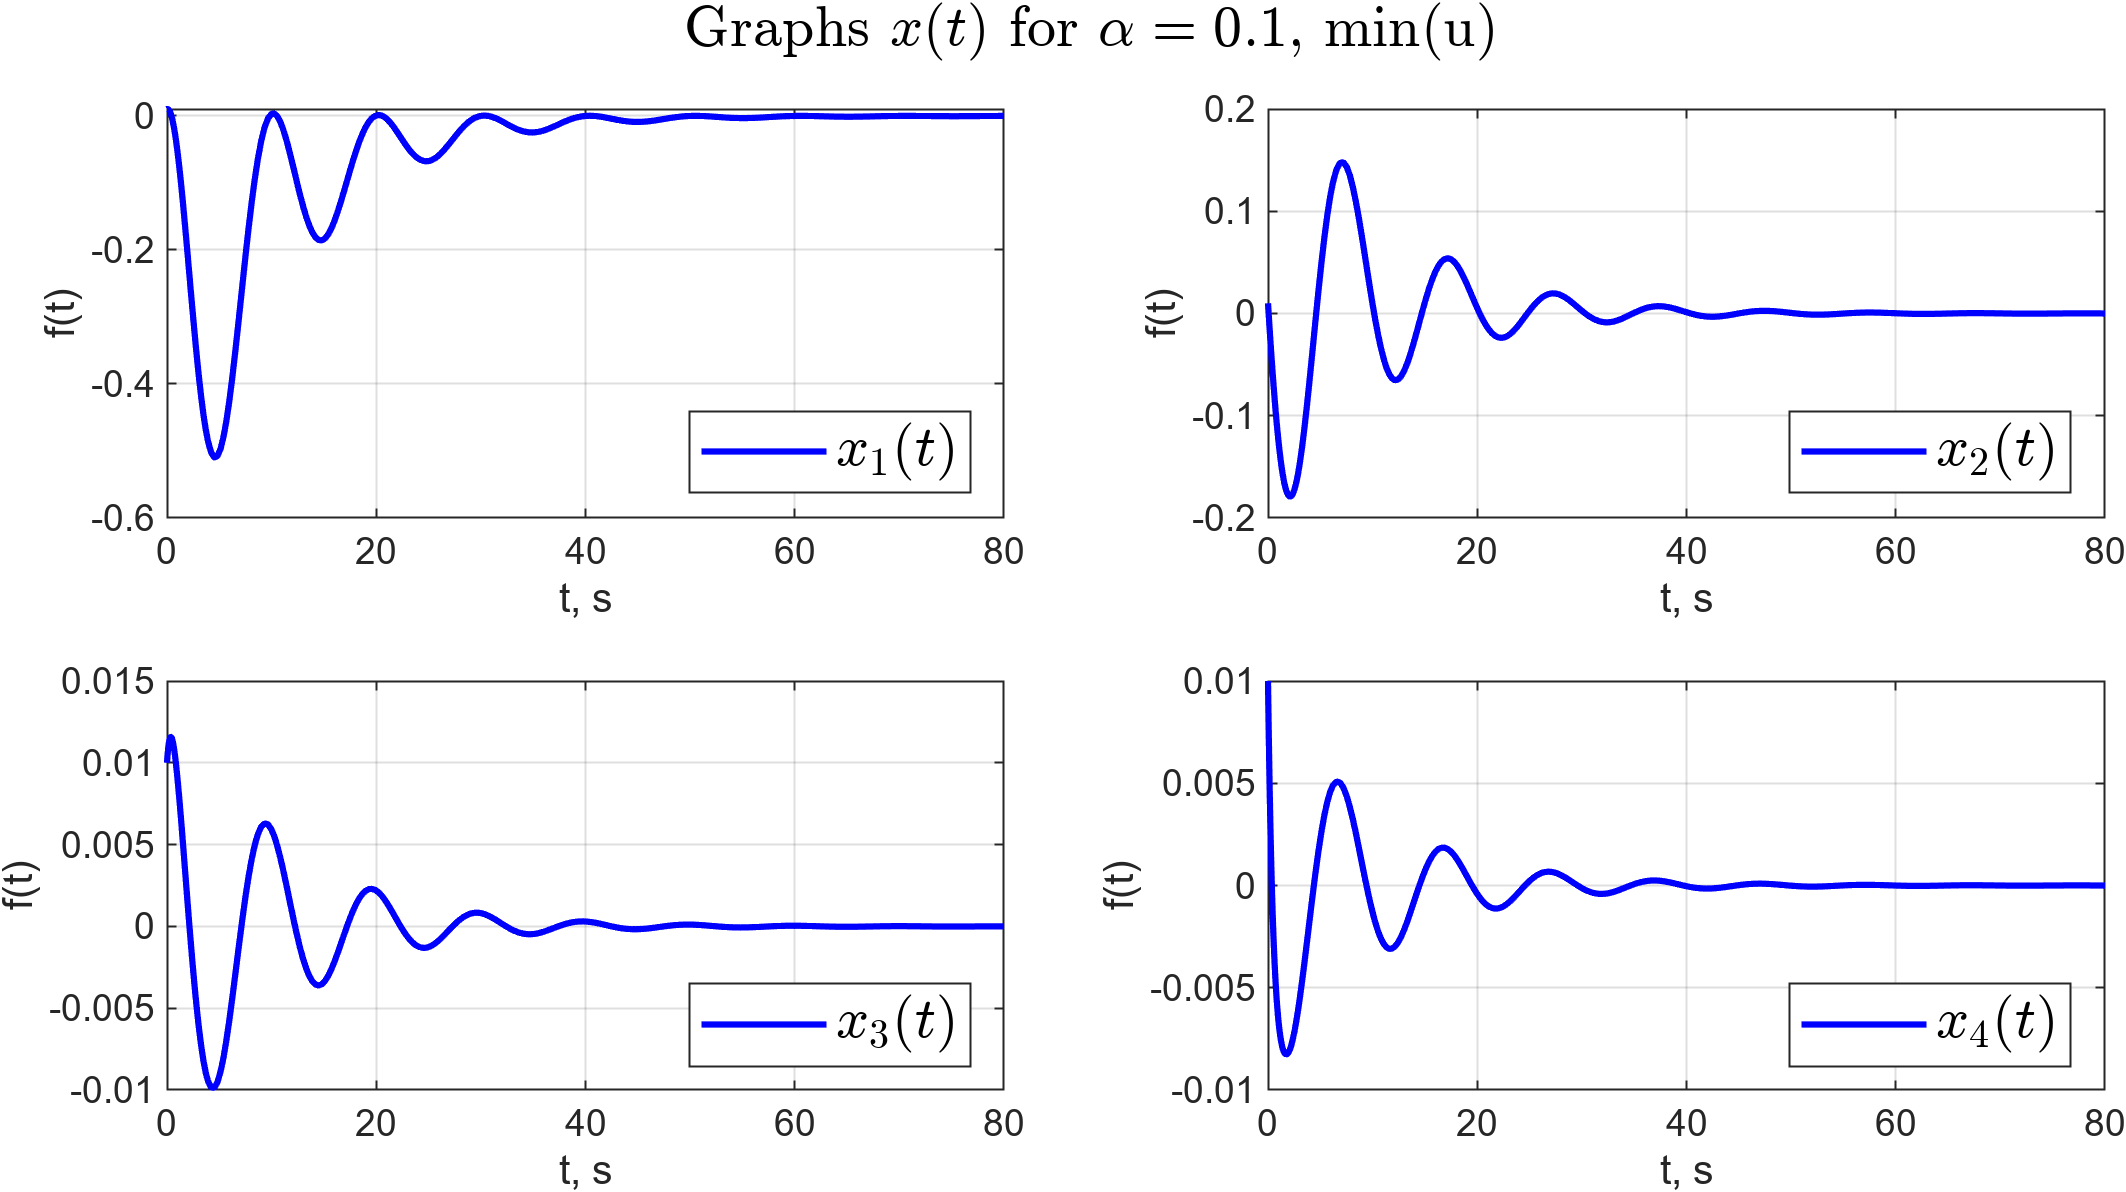
\includegraphics[width=1\linewidth]{pic/4_3_1.png}}
\caption{Графики $x(t)$, при $\alpha = 0.1$.}
\label{4_3_1}
\end{figure}




Для $\alpha_2=0.5$ матрица регулятора (моделирование -- рисунок \ref{4_3_2})

\begin{equation}
    K = \begin{bmatrix}
        142.6 & 400.8 & -5986 & -2492
    \end{bmatrix}
\end{equation}

\begin{figure}[!h]
\center{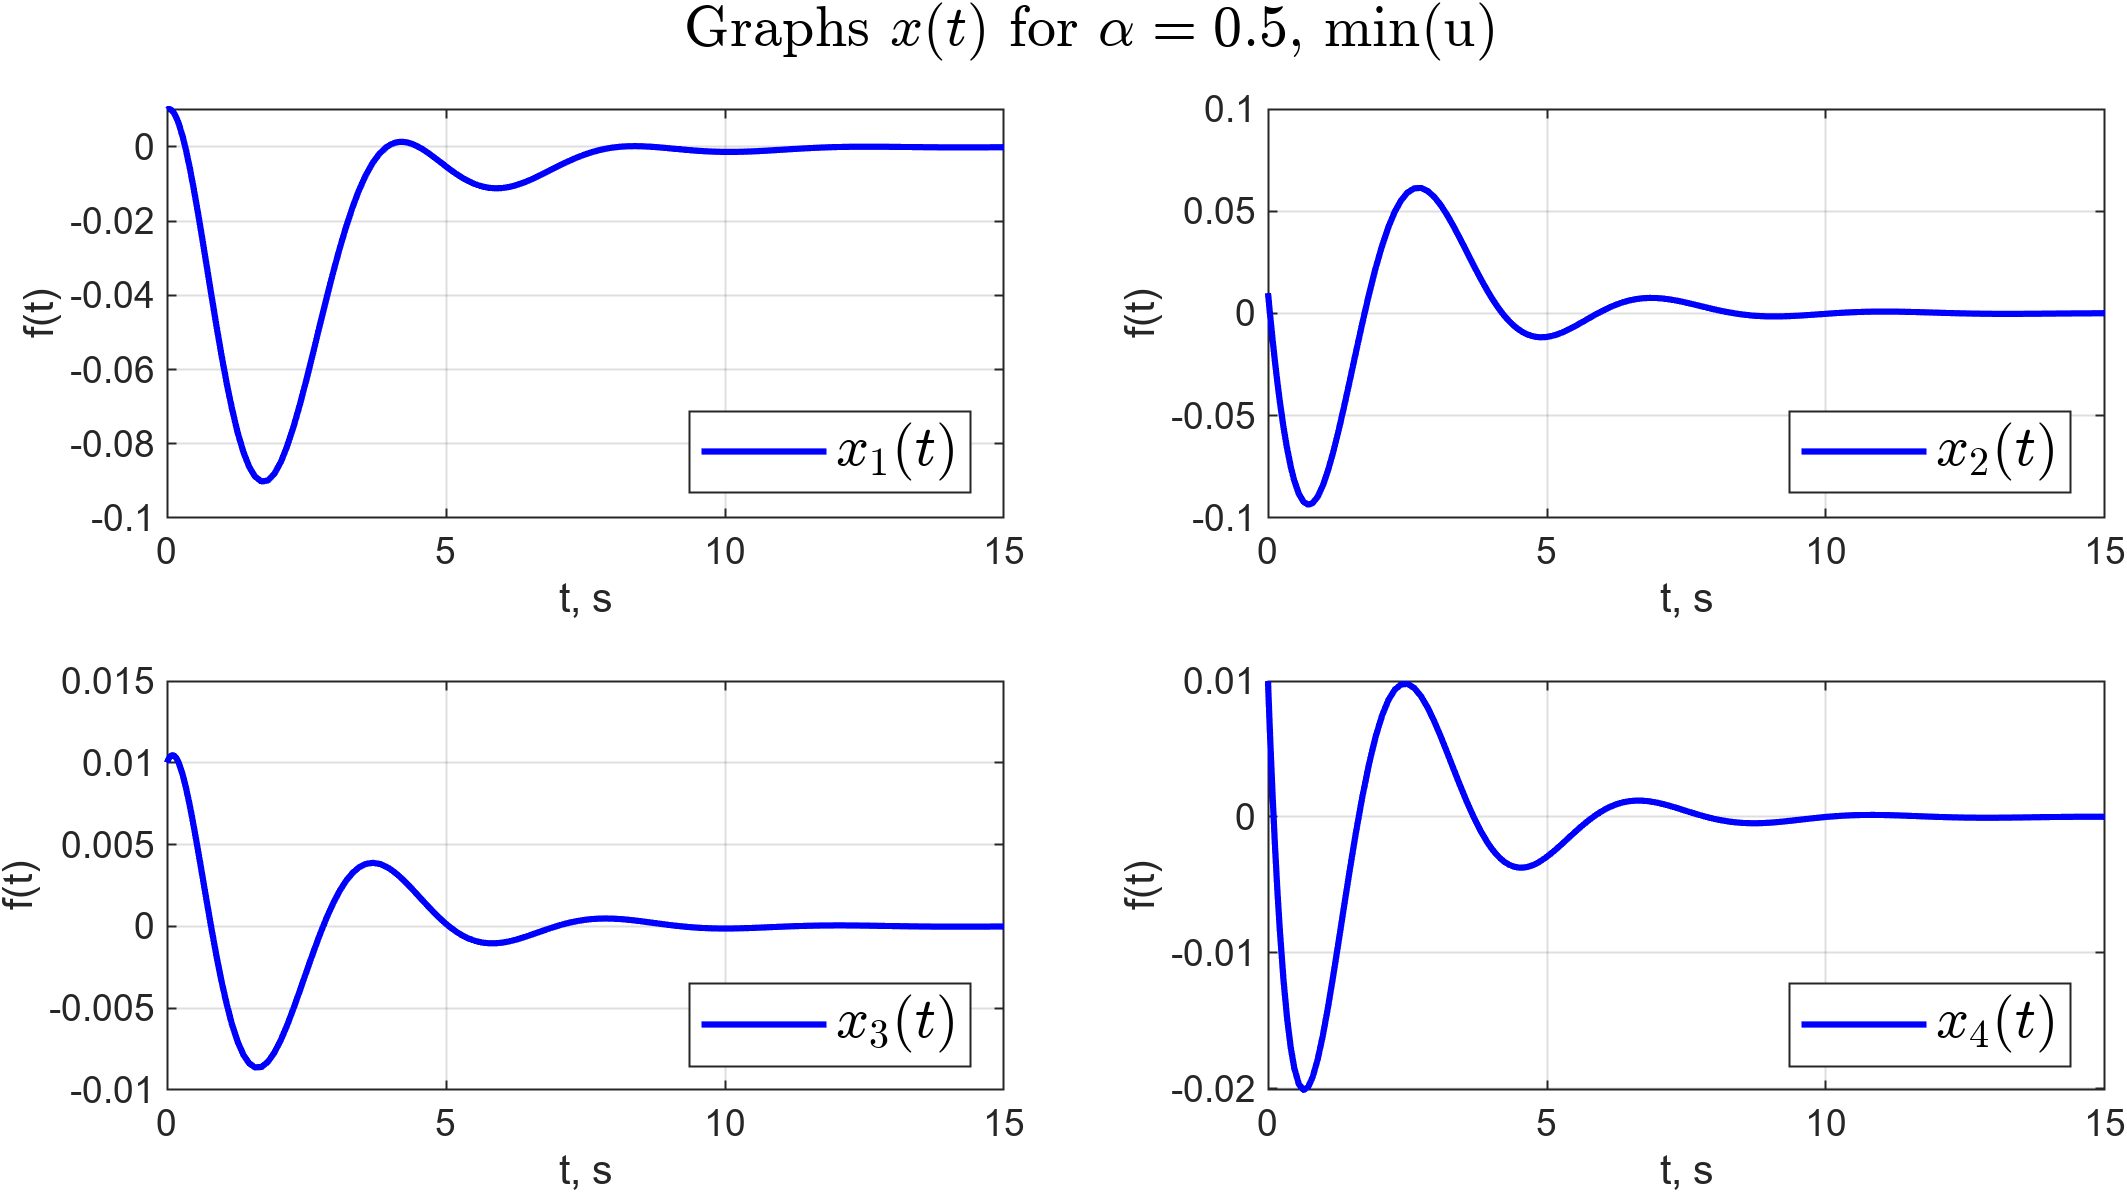
\includegraphics[width=1\linewidth]{pic/4_3_2.png}}
\caption{Графики $x(t)$, при $\alpha = 0.5$.}
\label{4_3_2}
\end{figure}


Для $\alpha_3=1$ матрица регулятора (моделирование -- рисунок \ref{4_3_3})

\begin{equation}
    K = \begin{bmatrix}
        718& 1242 & -11091 & -4631
    \end{bmatrix}
\end{equation}

\begin{figure}[!h]
\center{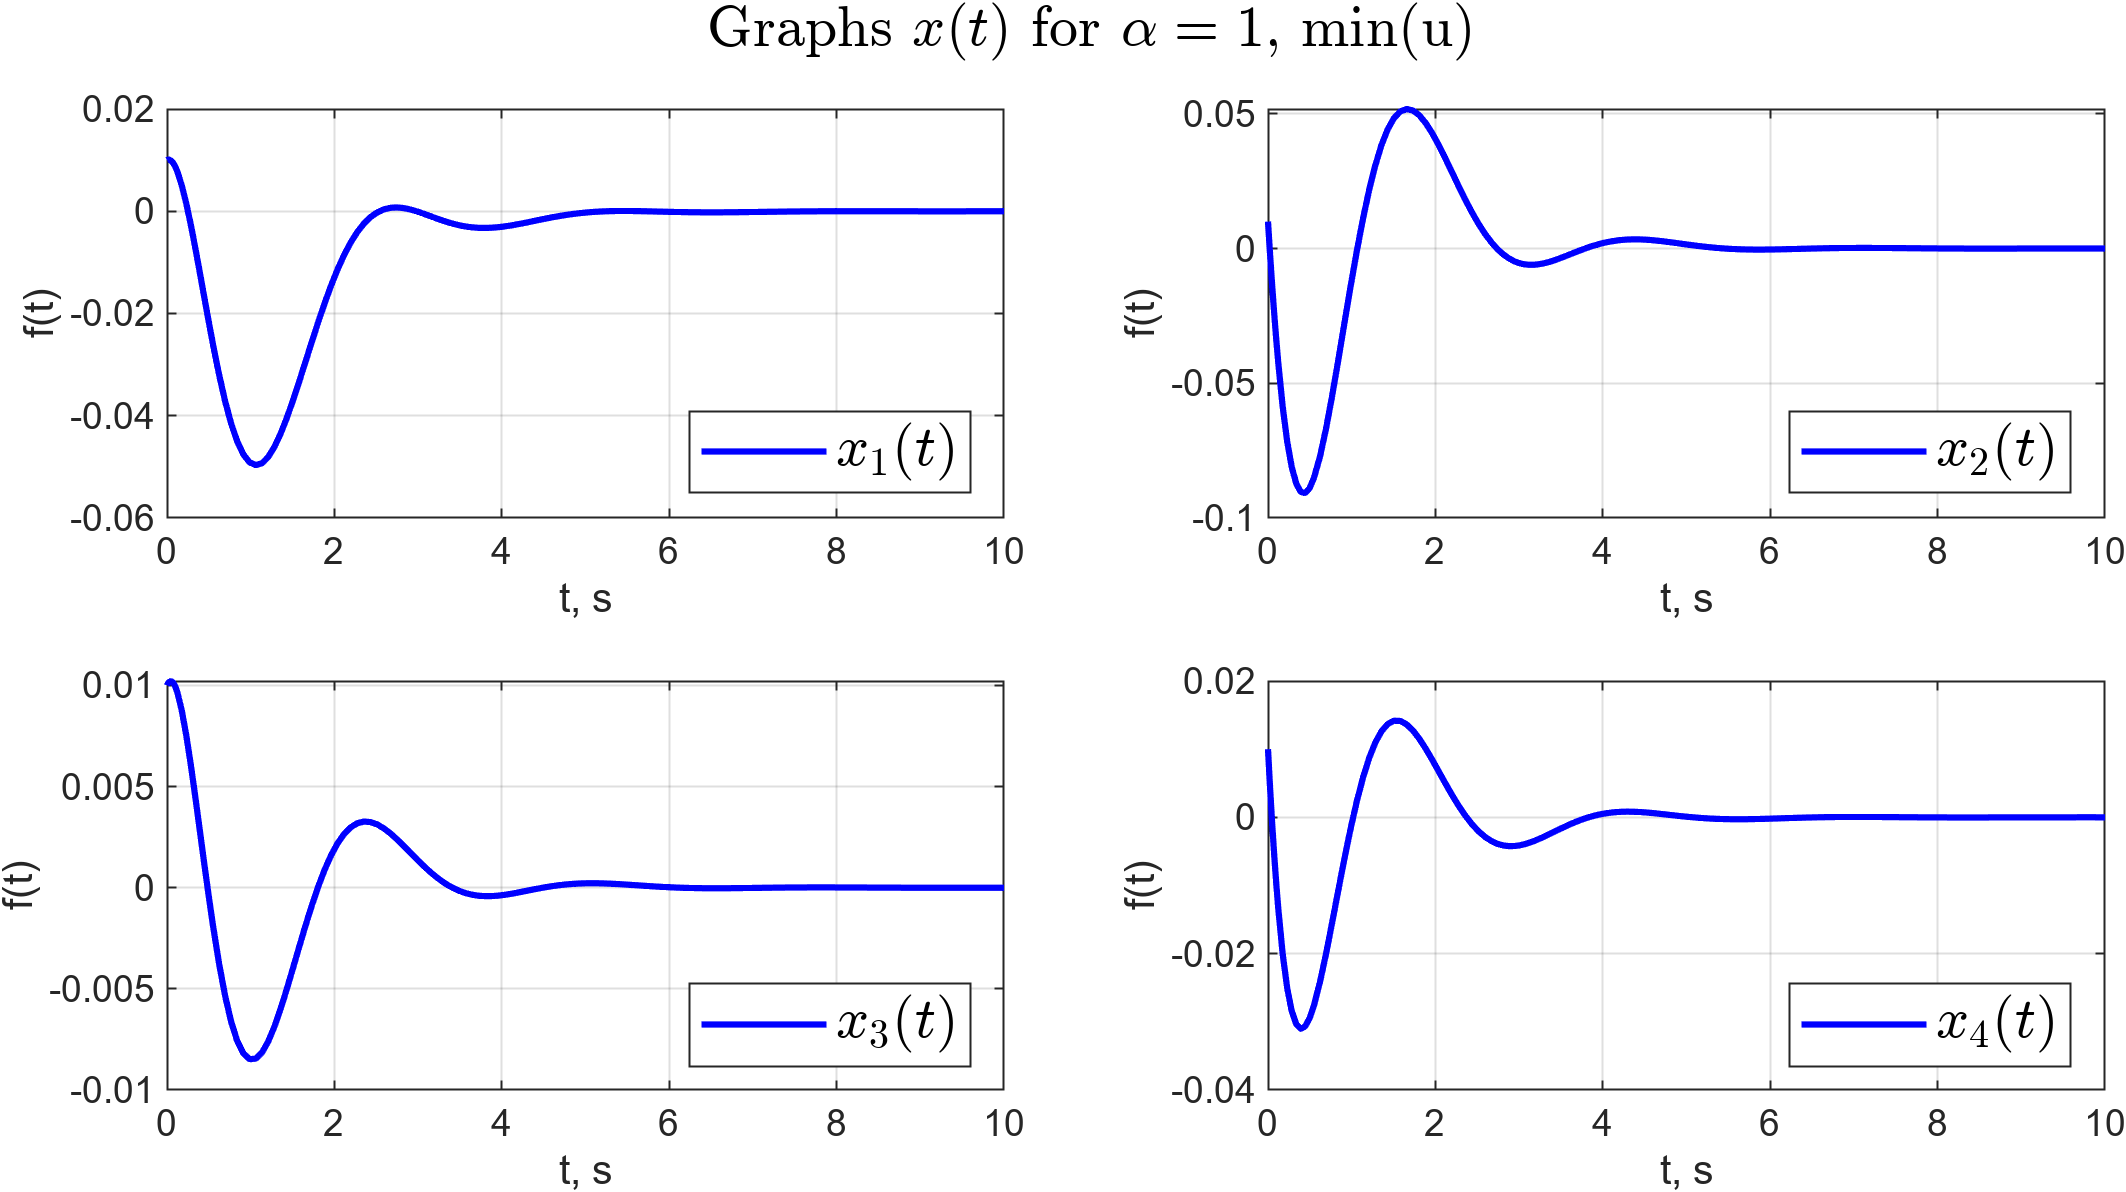
\includegraphics[width=1\linewidth]{pic/4_3_3.png}}
\caption{Графики $x(t)$, при $\alpha = 1$.}
\label{4_3_3}
\end{figure}


\newpage
При увеличении значения параметра $\alpha$ увеличиваются и значения матрицы $K$, но уменьшается время переходного процесса.

Для наглядности минимизации управления составим таблицу для $\alpha_{1,2,3}$ и соответствующих значений максимального модуля управления без решения задачи минимизации и после решения задачи (таблица \ref{4_tab_3}). Заметим, что задача минимизации управления действительно выполнена.

\begin{table}[h]
\centering
\caption{Результаты моделирования при разных значениях параметра $\alpha$.}
\label{4_tab_3}
\begin{tabular}{ccc}
\toprule
$\alpha$ & $\max |u|$ & $\max |u|$ with minimization\\
\midrule
0.1  &  66  &  45  \\
0.5  &  246  &  79   \\
1 &  304  &  138 \\ 
\bottomrule
\end{tabular}
\end{table}


Исследуем работоспособность синтезированного регулятора при управлении нелинейной системой в зависимости от начальных условий


\begin{equation*}
  \begin{matrix}
      x(0) = \begin{bmatrix}
          0.01 & 3 & 0.01 & 0.01
      \end{bmatrix}^T, & x(0) = \begin{bmatrix}
          0.01 & 0.01 & 0.01 & 0.1
      \end{bmatrix}^T,\\
      x(0) = \begin{bmatrix}
          0.01 & 0.01 & \pi /16 & 0.01
      \end{bmatrix}^T, & x(0) = \begin{bmatrix}
          5 & 0.01 & 0.01 & 0.1
      \end{bmatrix}^T,\\ 
 \end{matrix}
\end{equation*}

\begin{figure}[!h]
\center{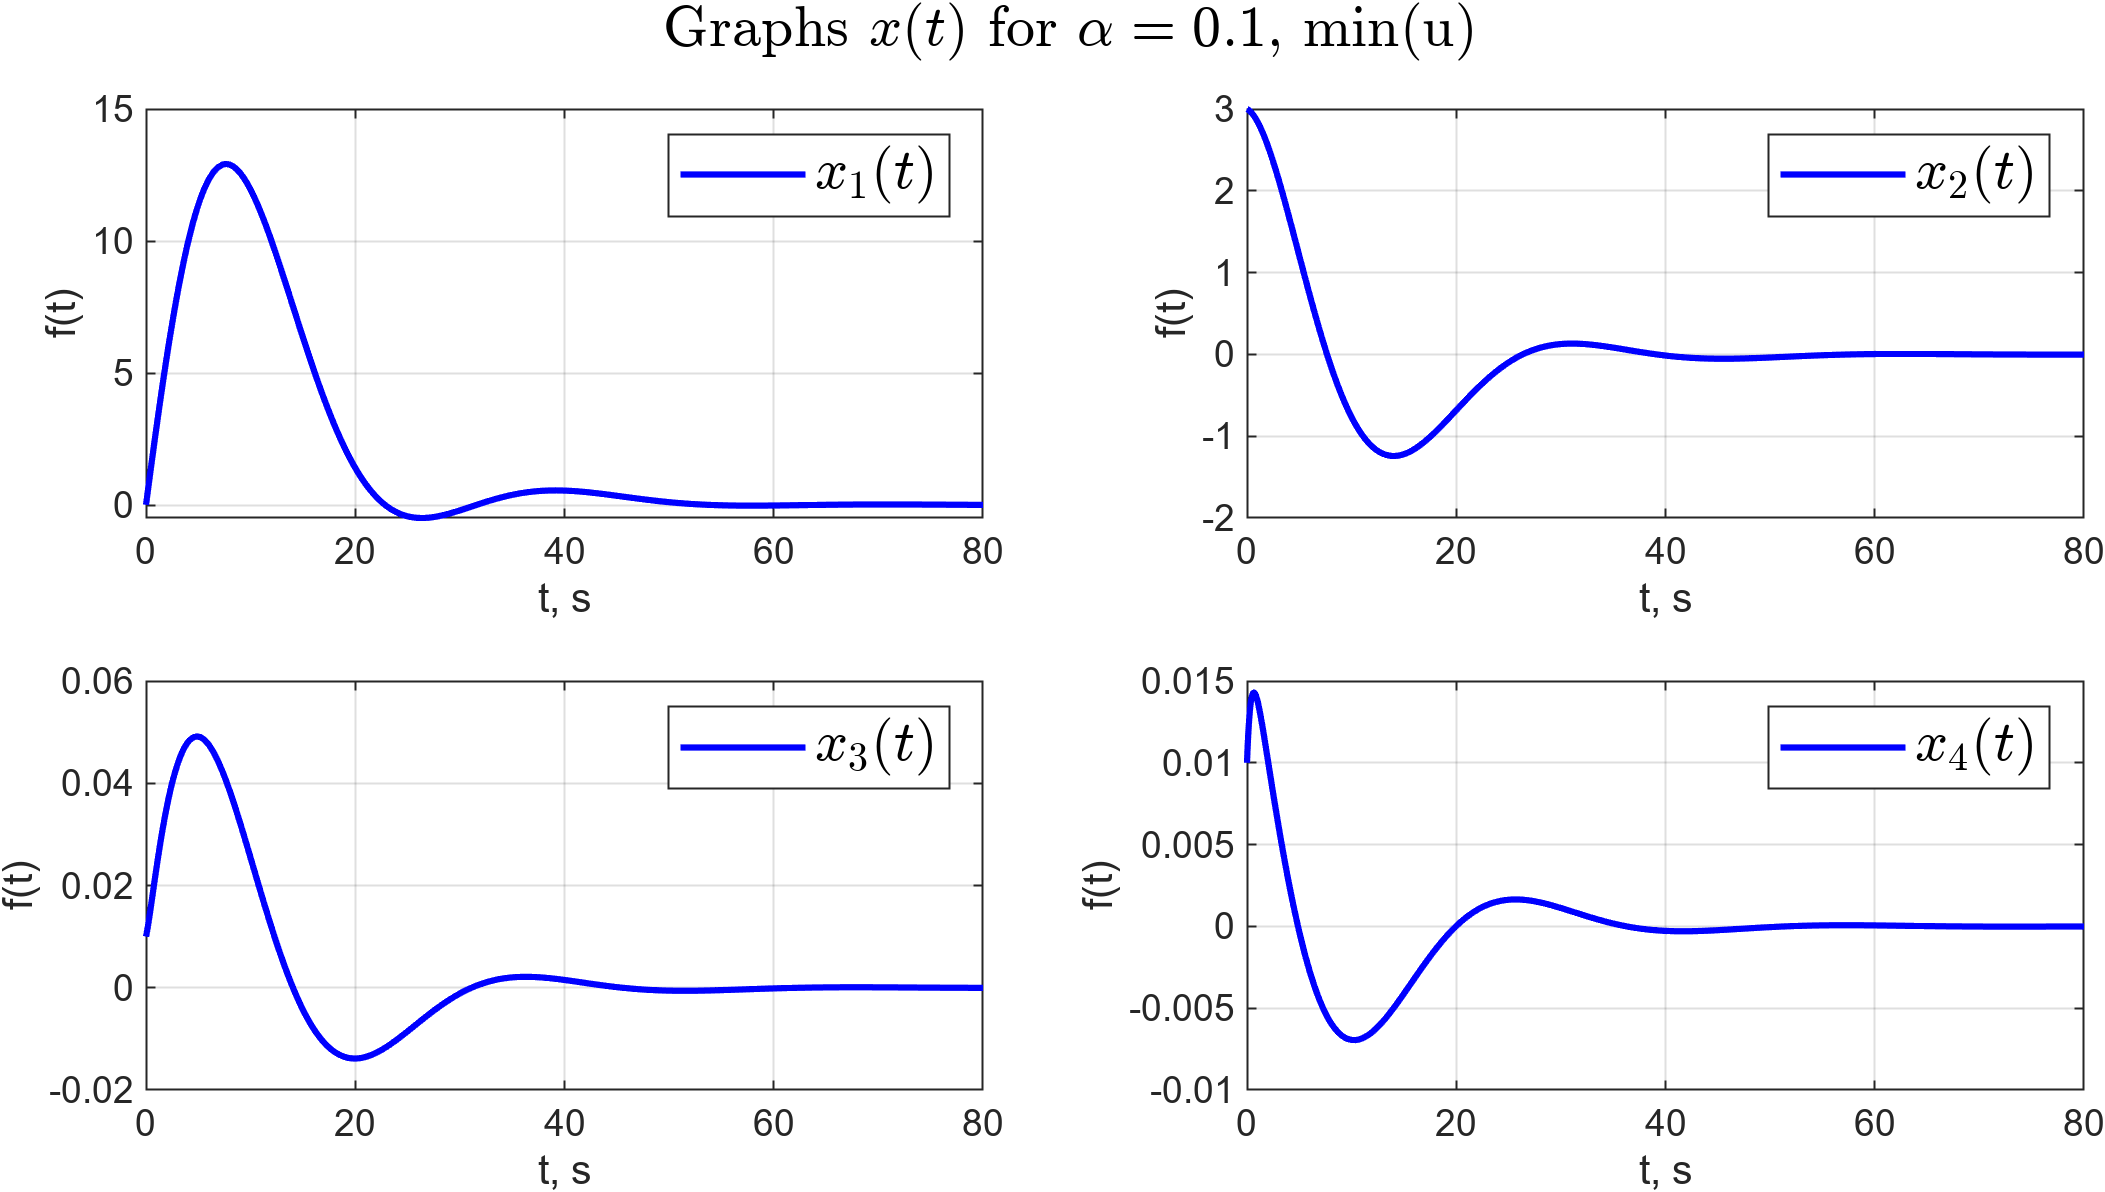
\includegraphics[width=1\linewidth]{pic/4_3_0.1_1.png}}
\caption{Графики $x(t)$, при $\alpha = 0.1$ и $x(0) = [0.01\, \, \,  3\, \, \, 0.01\, \, \, 0.01]^T$.}
\label{4_3_0.1_1}
\end{figure}


\begin{figure}[!h]
\center{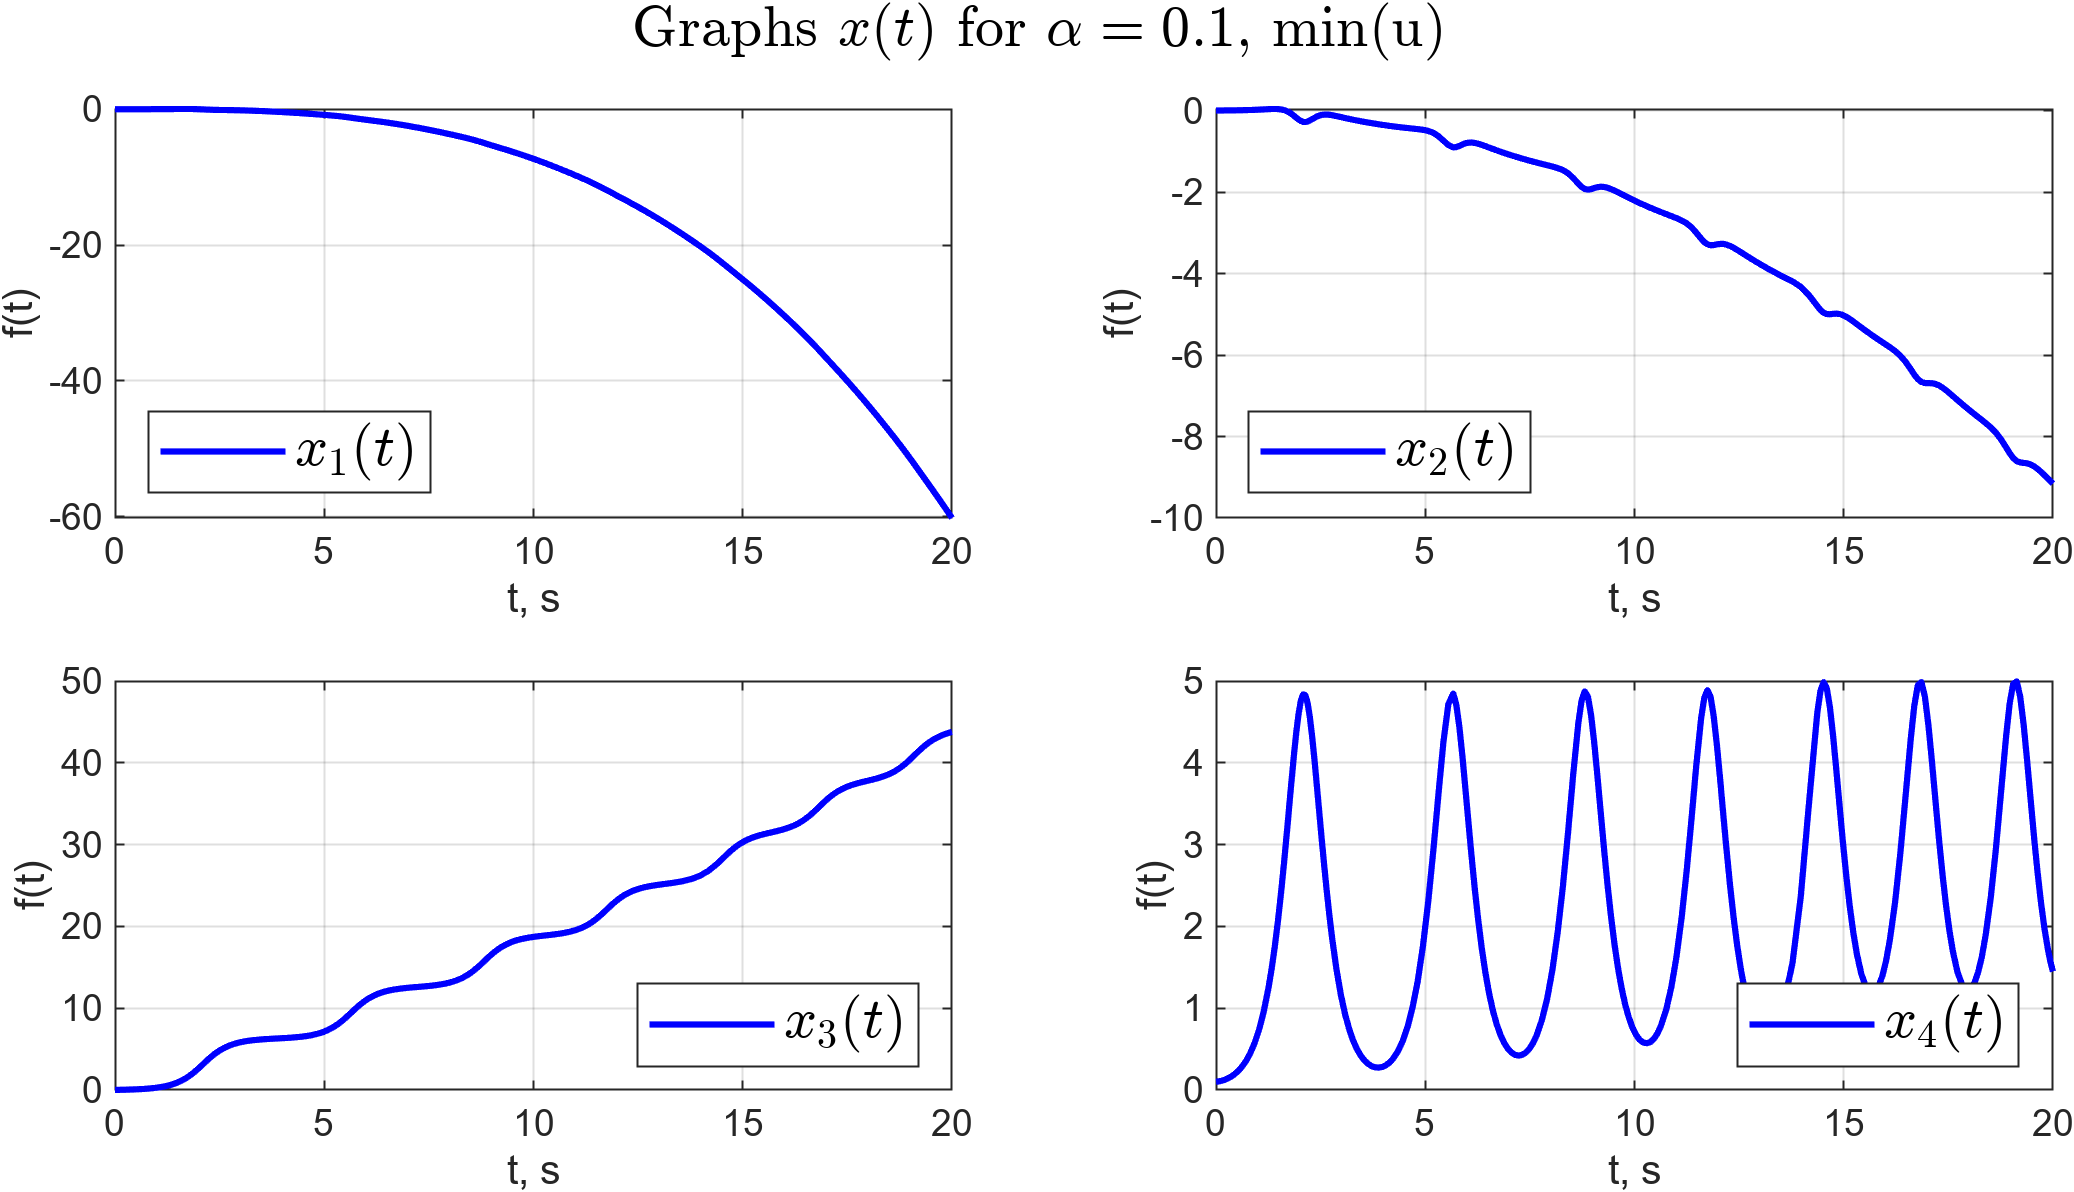
\includegraphics[width=1\linewidth]{pic/4_3_0.1_2.png}}
\caption{Графики $x(t)$, при $\alpha = 0.1$ и $x(0) = [0.01\, \, \,  0.01\, \, \, 0.01\, \, \, 0.1]^T$.}
\label{4_3_0.1_2}
\end{figure}

Заметим, что значение начальной угловой скорости $0.1$ рад/с оказывается слишком большим для регулятора (рисунок \ref{4_3_0.1_2}). Кроме того, для больших значений начальной угловой скорости решения не существует. Аналогичный случай с начальным углом: максимальное значение, при котором существует решение системы $\pi /16$, здесь регулятор также не справляется с задачей стабилизации (рисунок \ref{4_3_0.1_3}).

\begin{figure}[!h]
\center{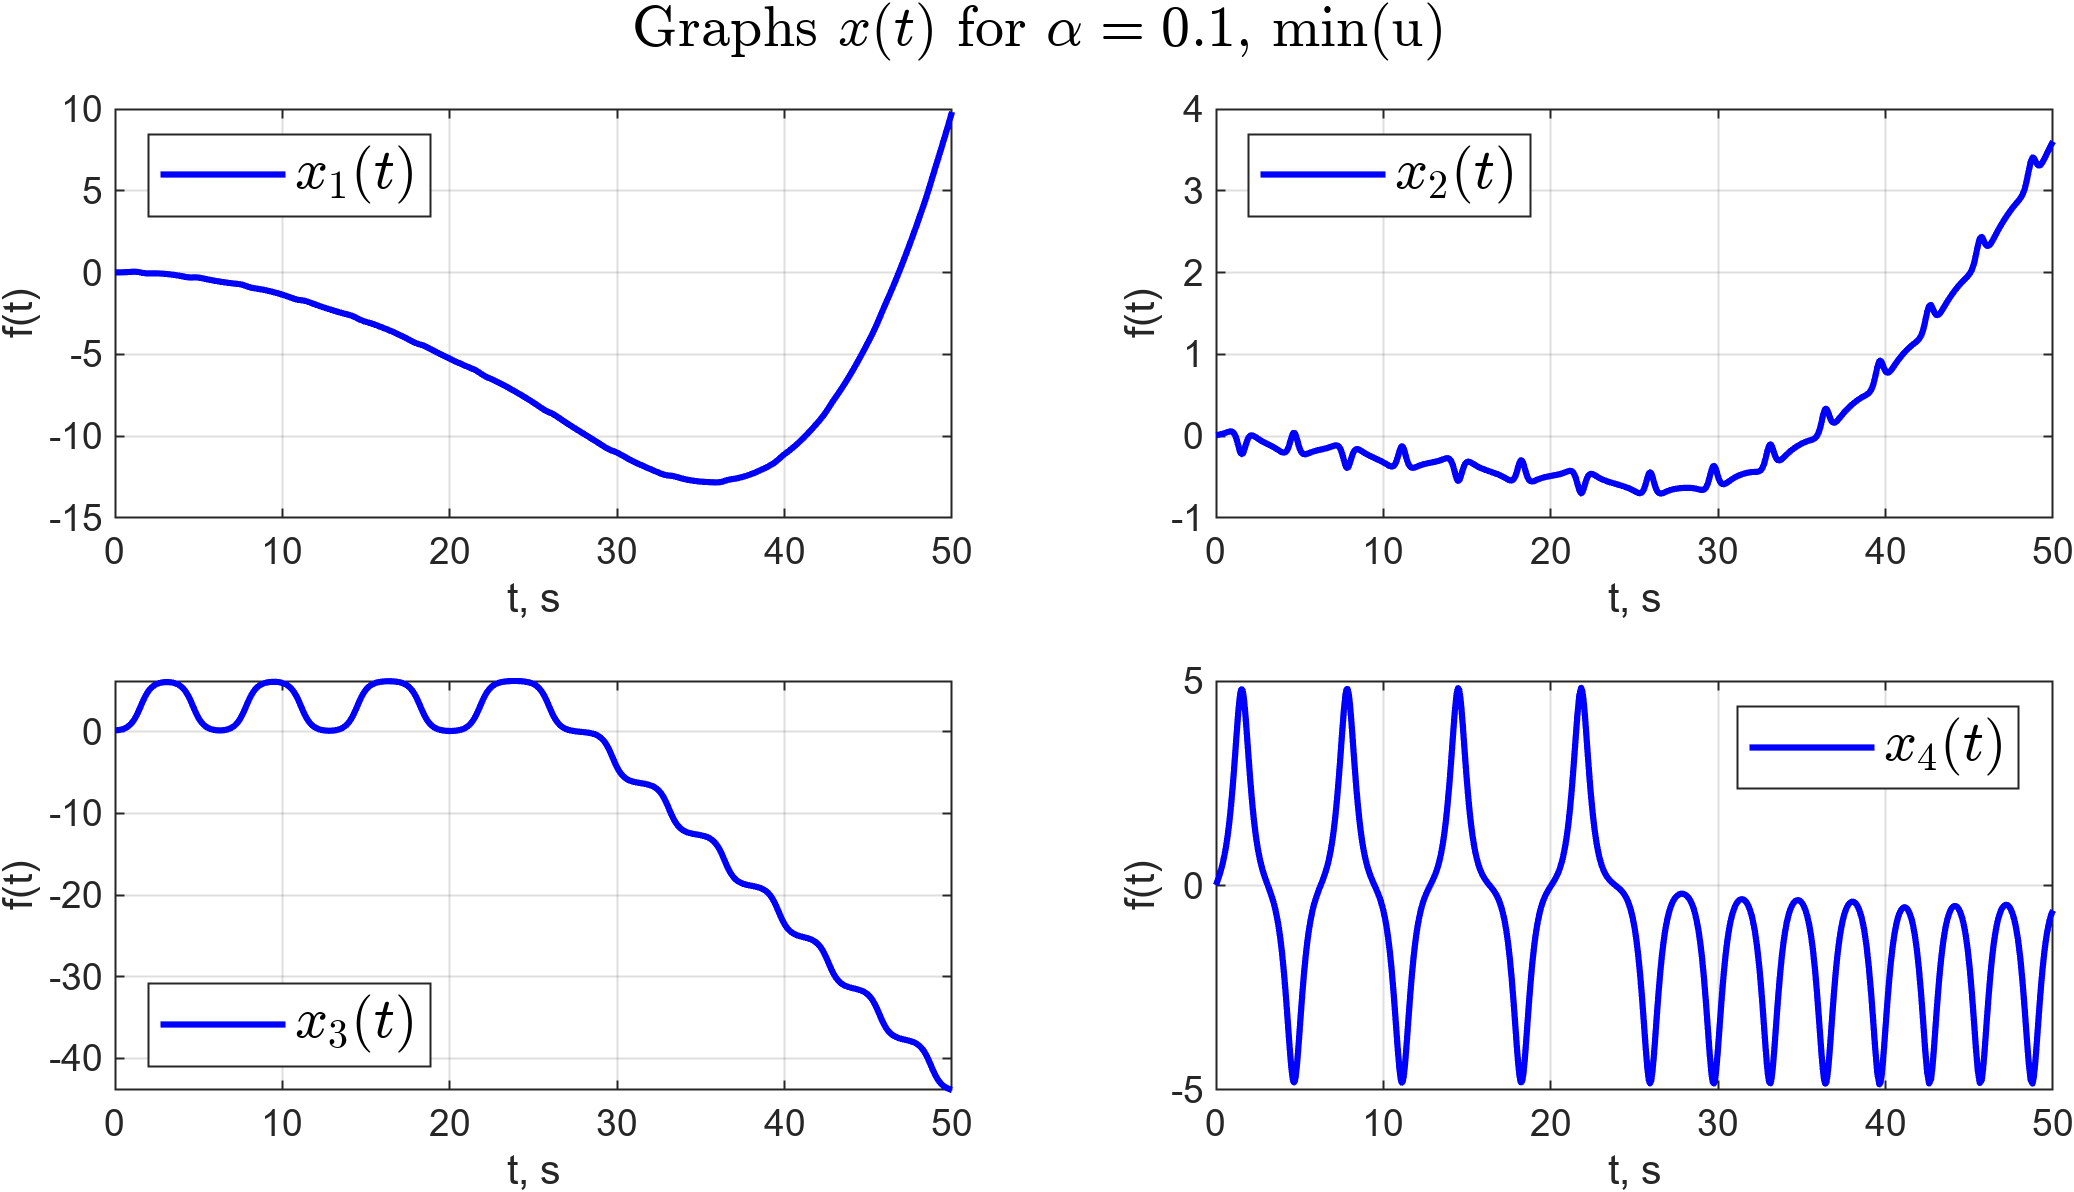
\includegraphics[width=1\linewidth]{pic/4_3_0.1_3.png}}
\caption{Графики $x(t)$, при $\alpha = 0.1$ и $x(0) = [0.01\, \, \,  0.01\, \, \, \pi /16\, \, \, 0.01]^T$.}
\label{4_3_0.1_3}
\end{figure}


\begin{figure}[!h]
\center{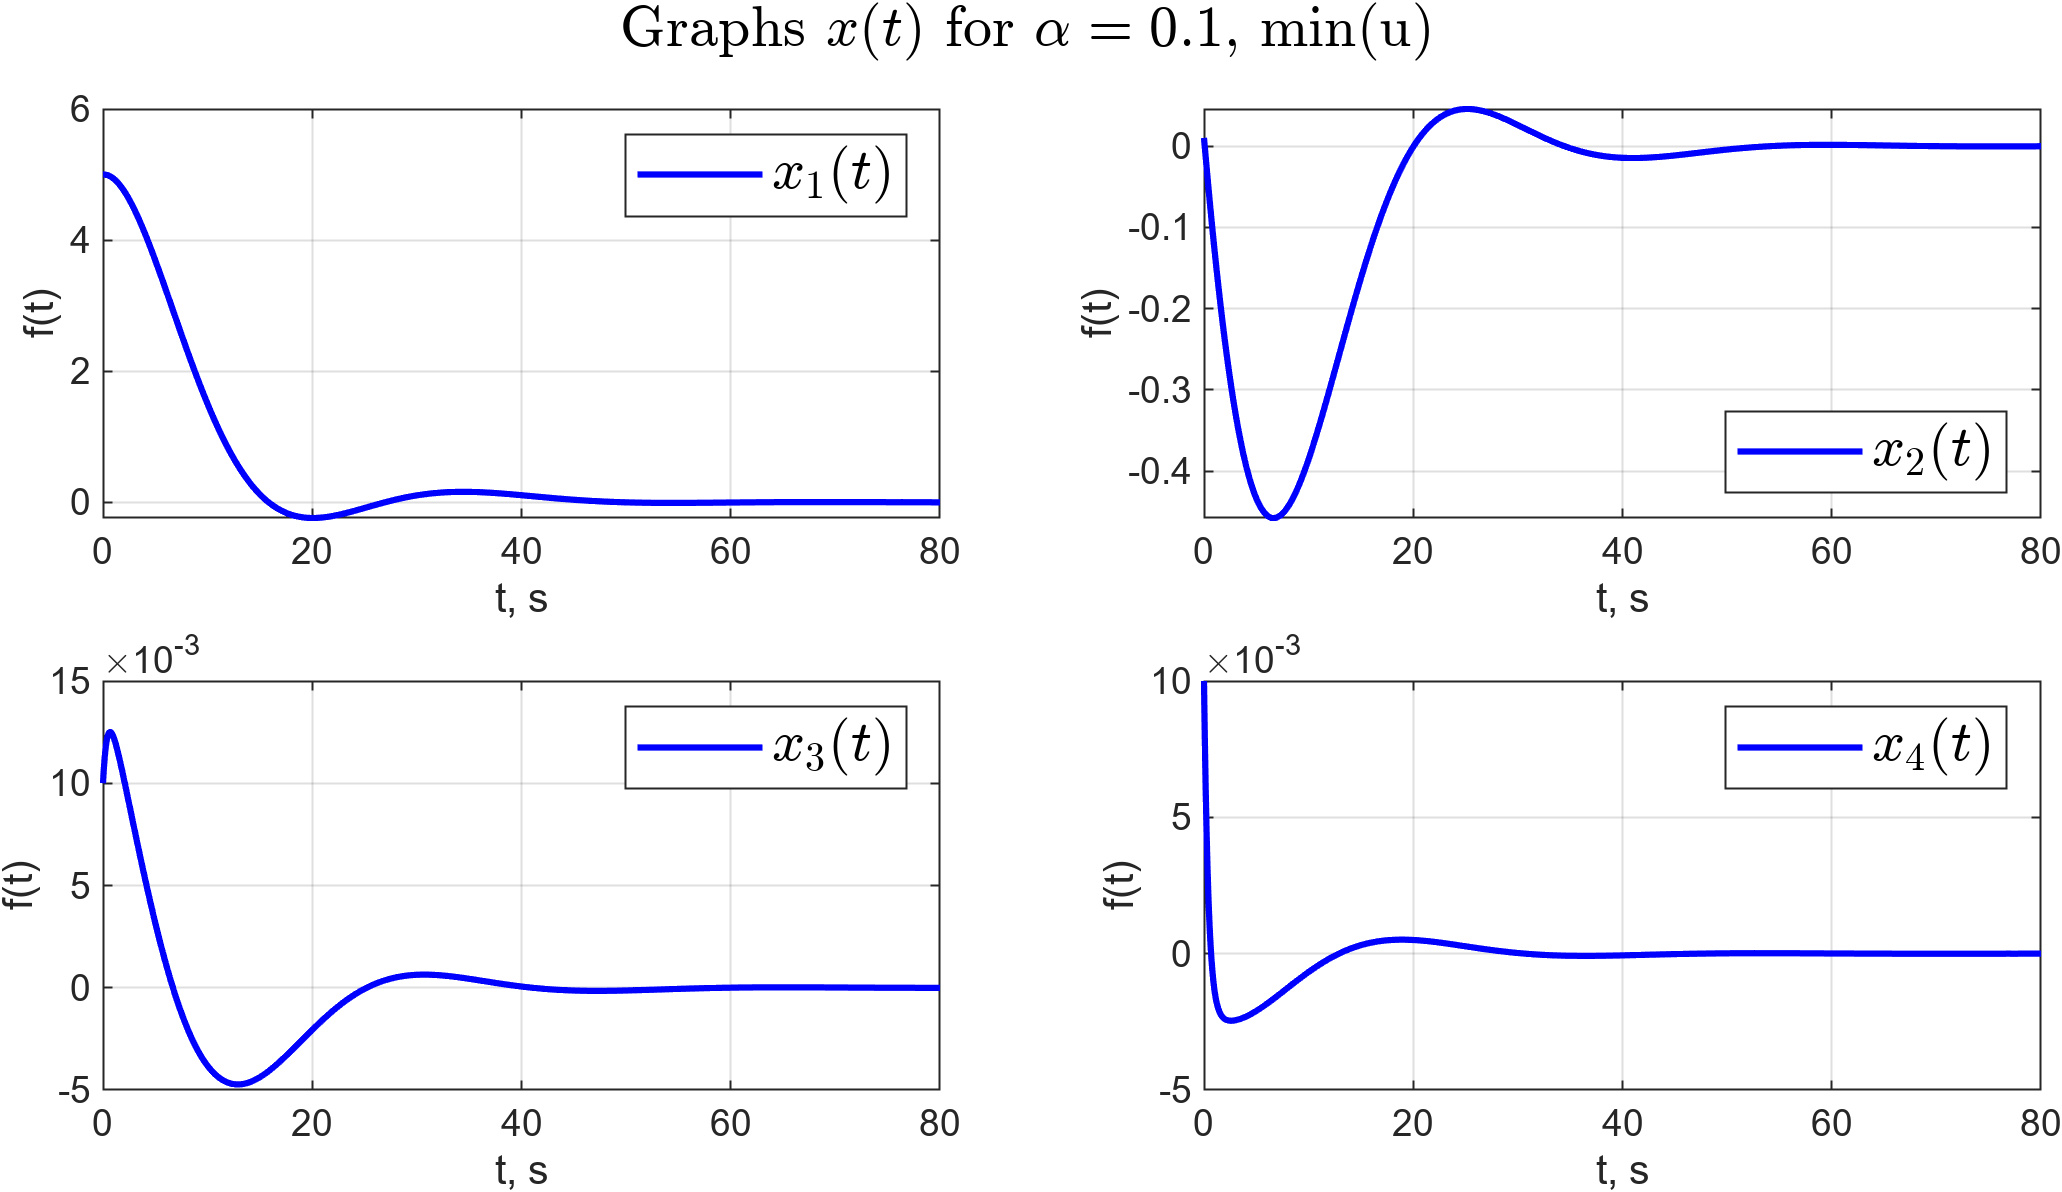
\includegraphics[width=1\linewidth]{pic/4_3_0.1_4.png}}
\caption{Графики $x(t)$, при $\alpha = 0.1$ и $x(0) = [5\, \, \,  0.01\, \, \, 0.01\, \, \, 0.01]^T$.}
\label{4_3_0.1_4}
\end{figure}

\newpage
Для начального условия $x(0)=\begin{bmatrix}
          0.01 & 3 & 0.01 & 0.01
      \end{bmatrix}^T$ не существует решения для $\alpha_2 = 0.5$, поэтому выполним моделирование для $x(0)=\begin{bmatrix}
          0.01 & 1 & 0.01 & 0.01
      \end{bmatrix}^T$


\begin{figure}[!h]
\center{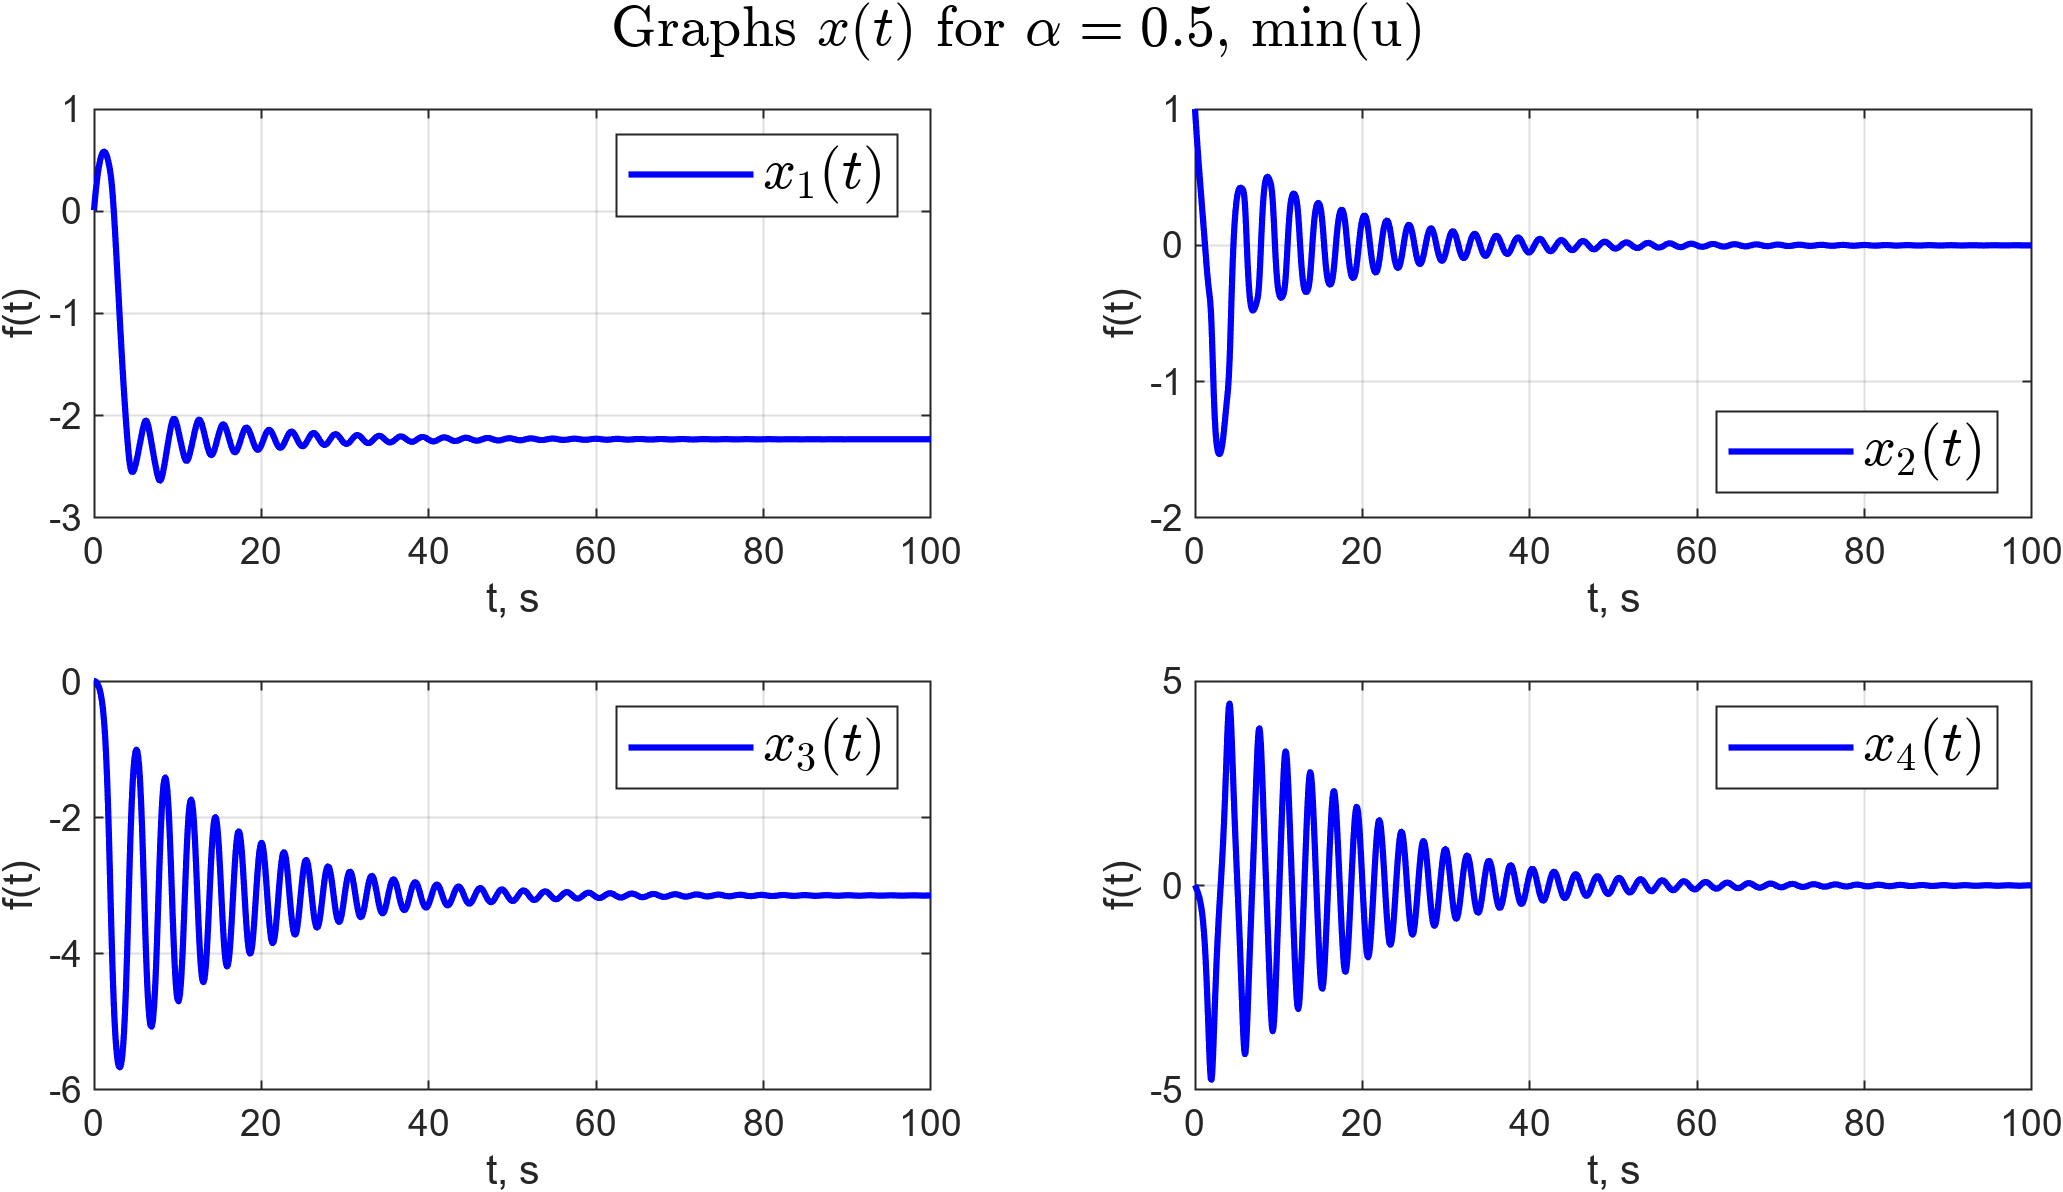
\includegraphics[width=1\linewidth]{pic/4_3_0.5_1.png}}
\caption{Графики $x(t)$, при $\alpha = 0.5$ и $x(0) = [0.01\, \, \,  1\, \, \, 0.01\, \, \, 0.01]^T$.}
\label{4_3_0.5_1}
\end{figure}


\begin{figure}[!h]
\center{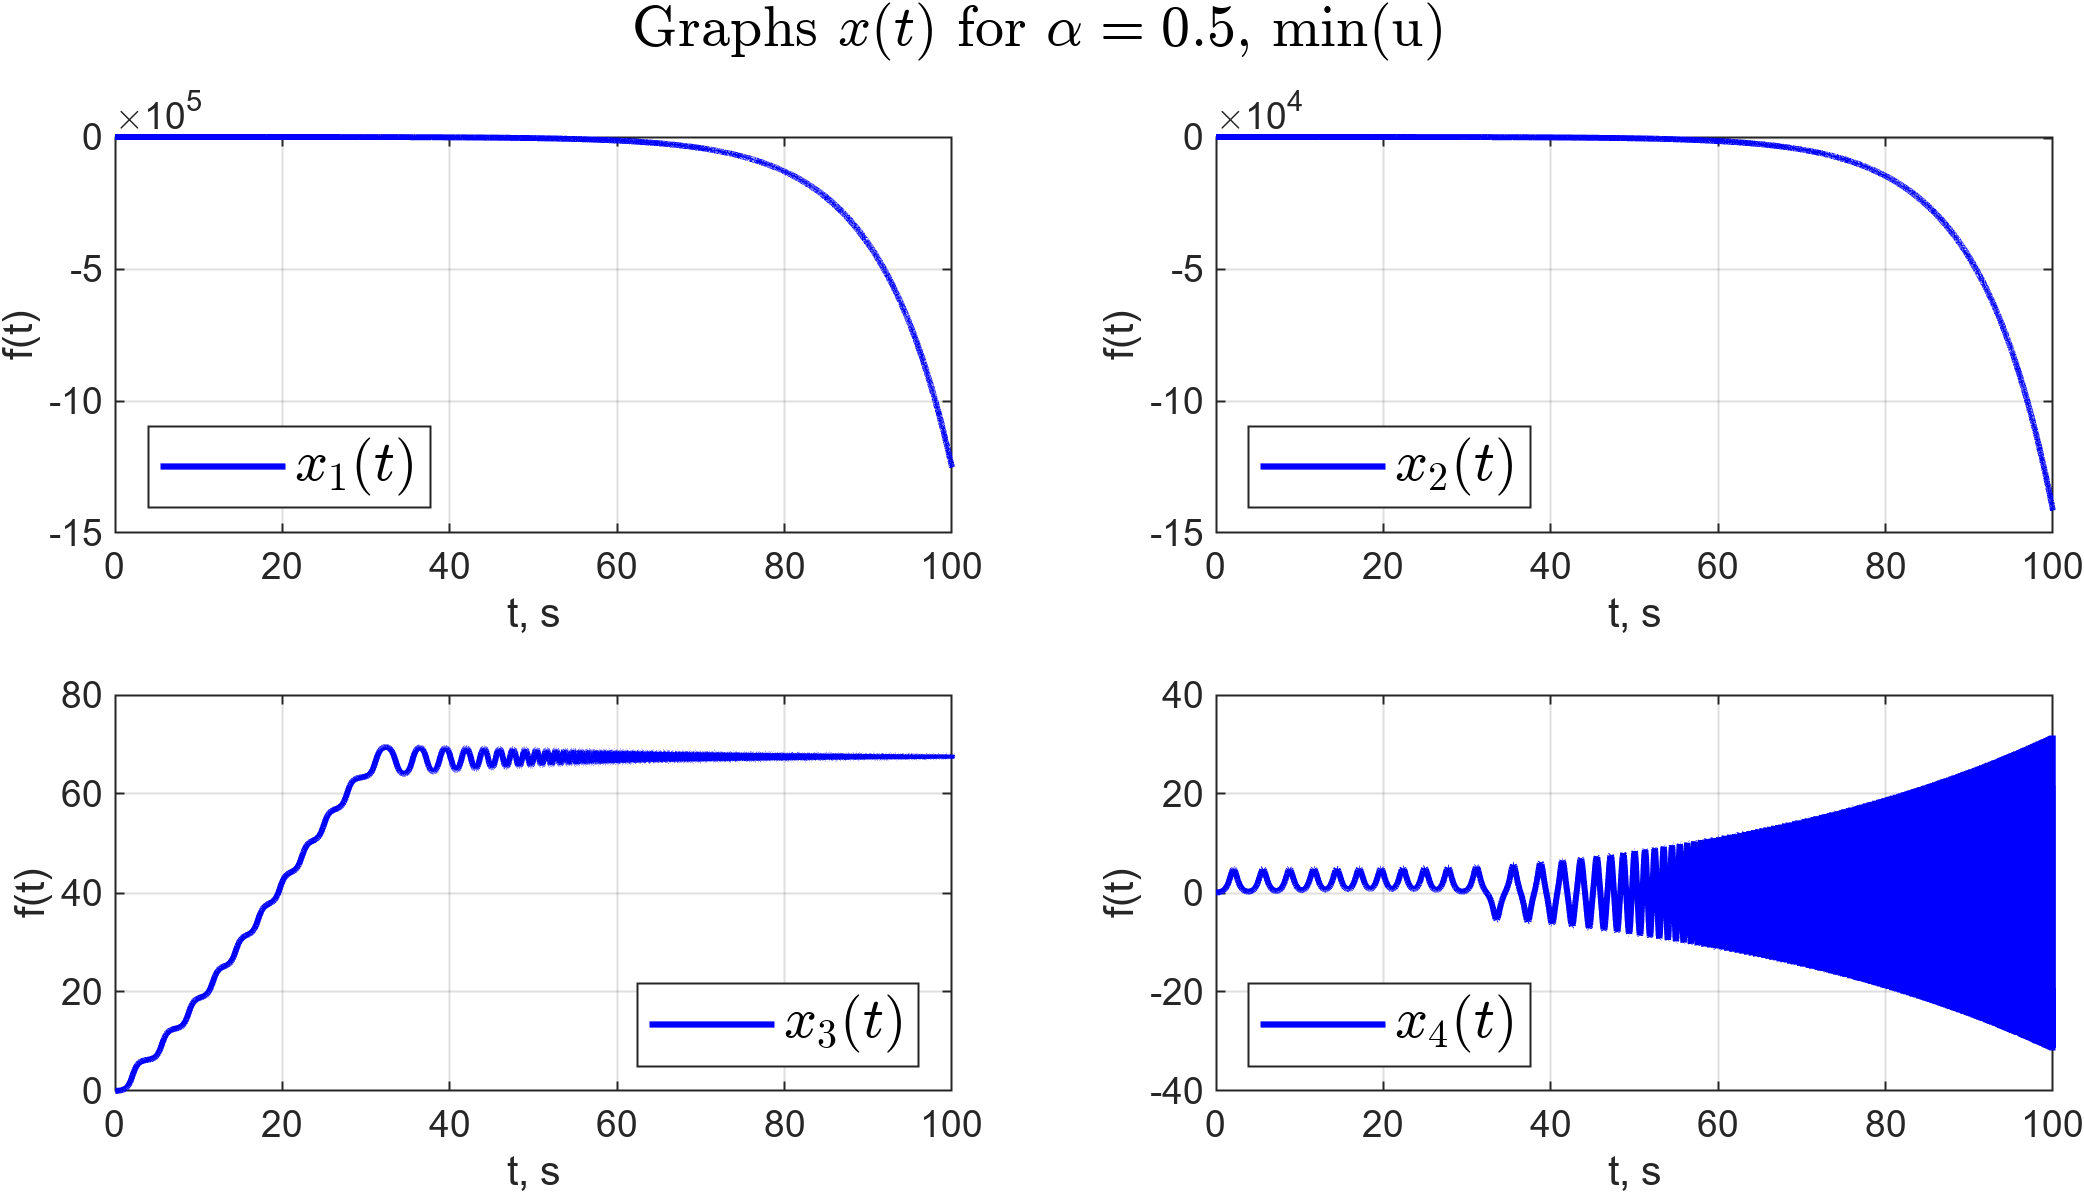
\includegraphics[width=1\linewidth]{pic/4_3_0.5_2.png}}
\caption{Графики $x(t)$, при $\alpha = 0.5$ и $x(0) = [0.01\, \, \,  0.01\, \, \, 0.01\, \, \, 0.1]^T$.}
\label{4_3_0.5_2}
\end{figure}

Заметим, что начальная угловая скорость $0.1$ рад/с, слишком большая для того, чтобы регулятор с $\alpha_2 = 0.5$ и минимальным управлением справился с задачей стабилизации (рисунок \ref{4_3_0.5_2}).

Для начального значения угла отклонения маятника $\pi /16$ также не существует решения системы неравенств, возьмем максимальный угол, при котором система имеет решение $\pi /17$, однако система расходится (рисунок \ref{4_3_0.5_3})

\begin{figure}[!h]
\center{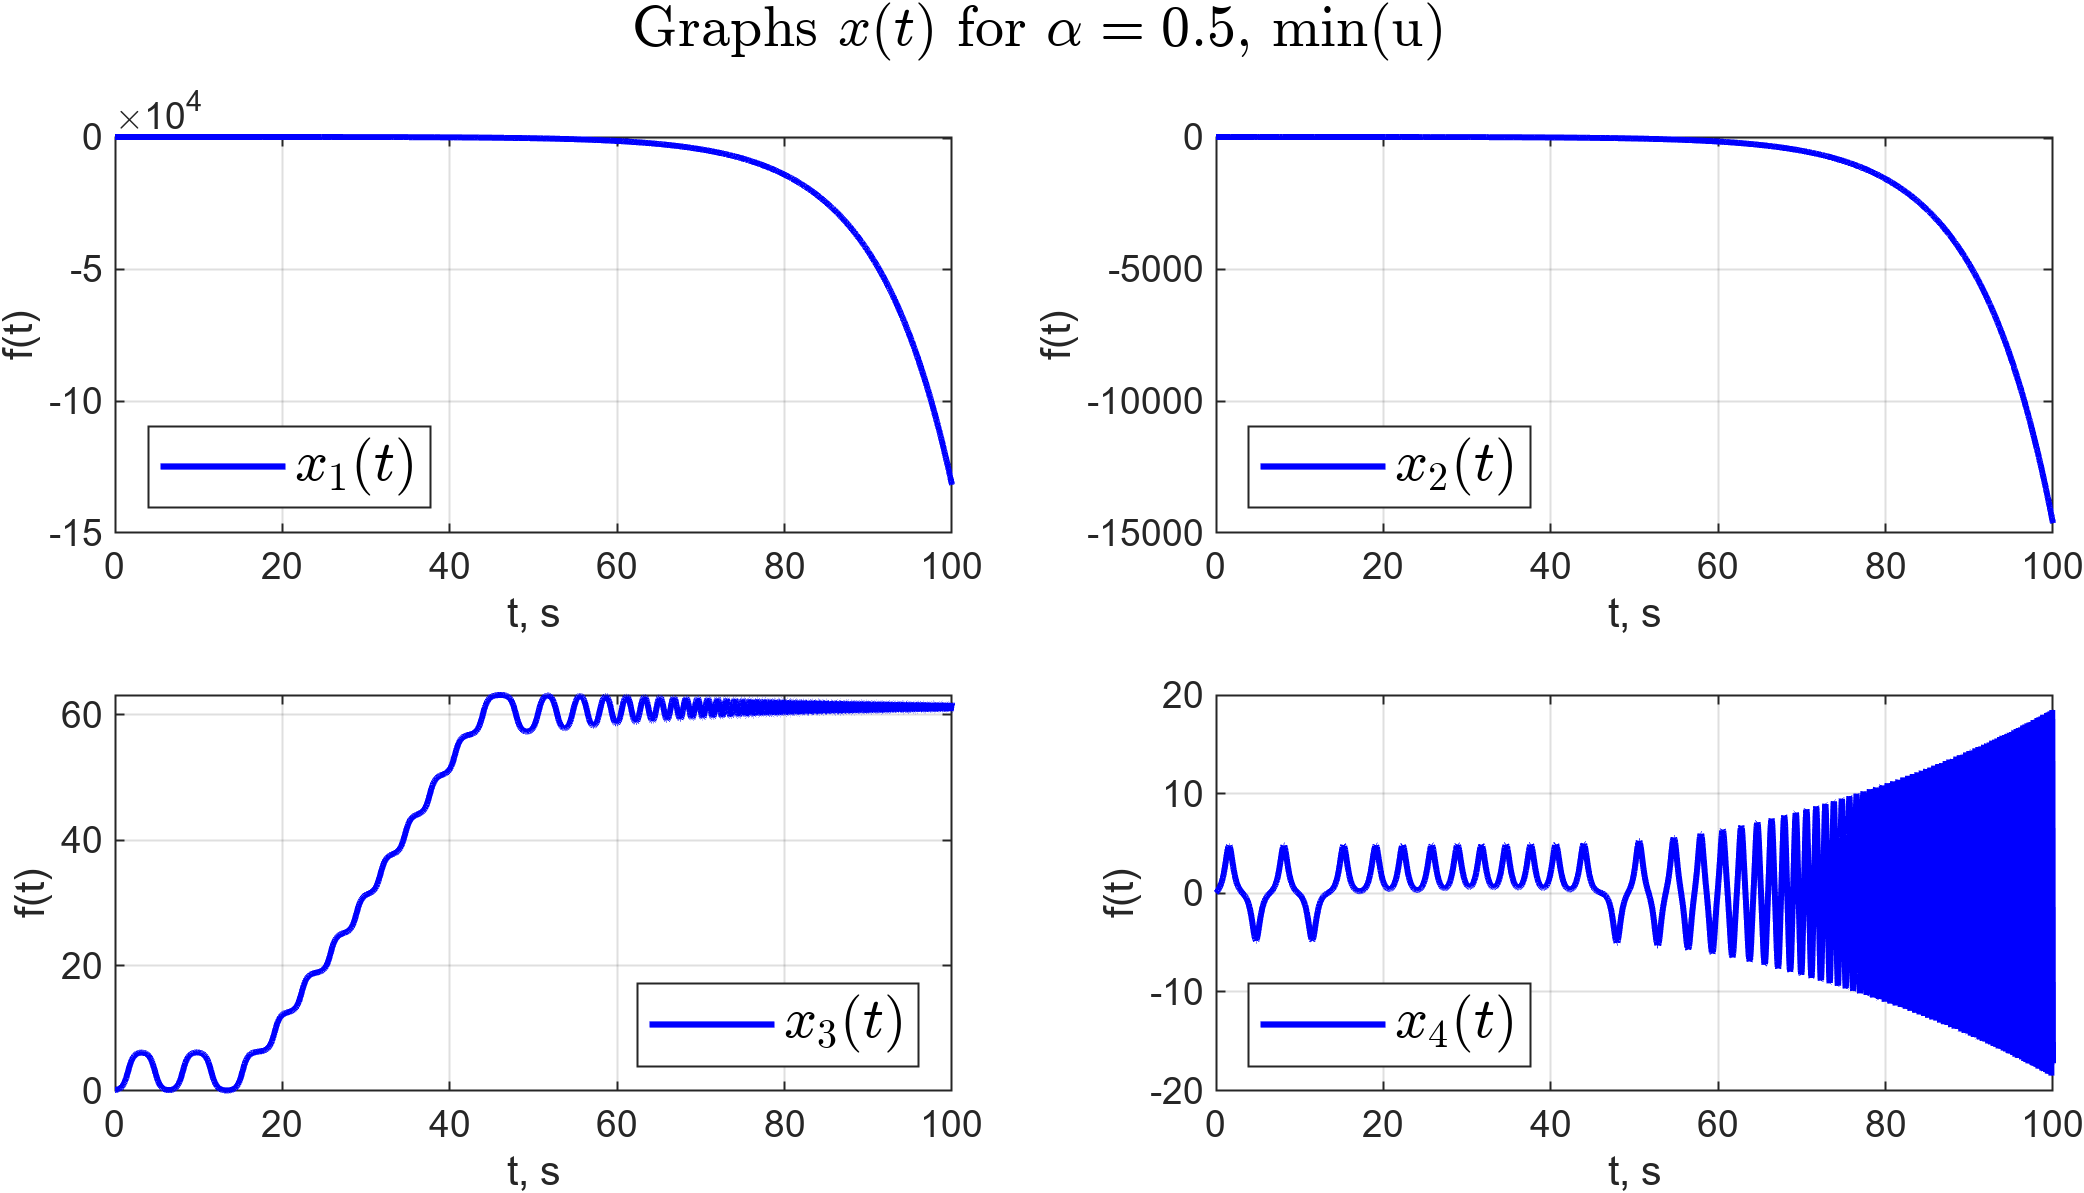
\includegraphics[width=1\linewidth]{pic/4_3_0.5_3.png}}
\caption{Графики $x(t)$, при $\alpha = 0.5$ и $x(0) = [0.01\, \, \,  0.01\, \, \, \pi / 17\, \, \, 0.01]^T$.}
\label{4_3_0.5_3}
\end{figure}


Аналогично для начального значения координаты тележки $5$ м система неравенств не имеет решения, возьмем значение $2$ м в качестве начальной координаты тележки

\begin{figure}[!h]
\center{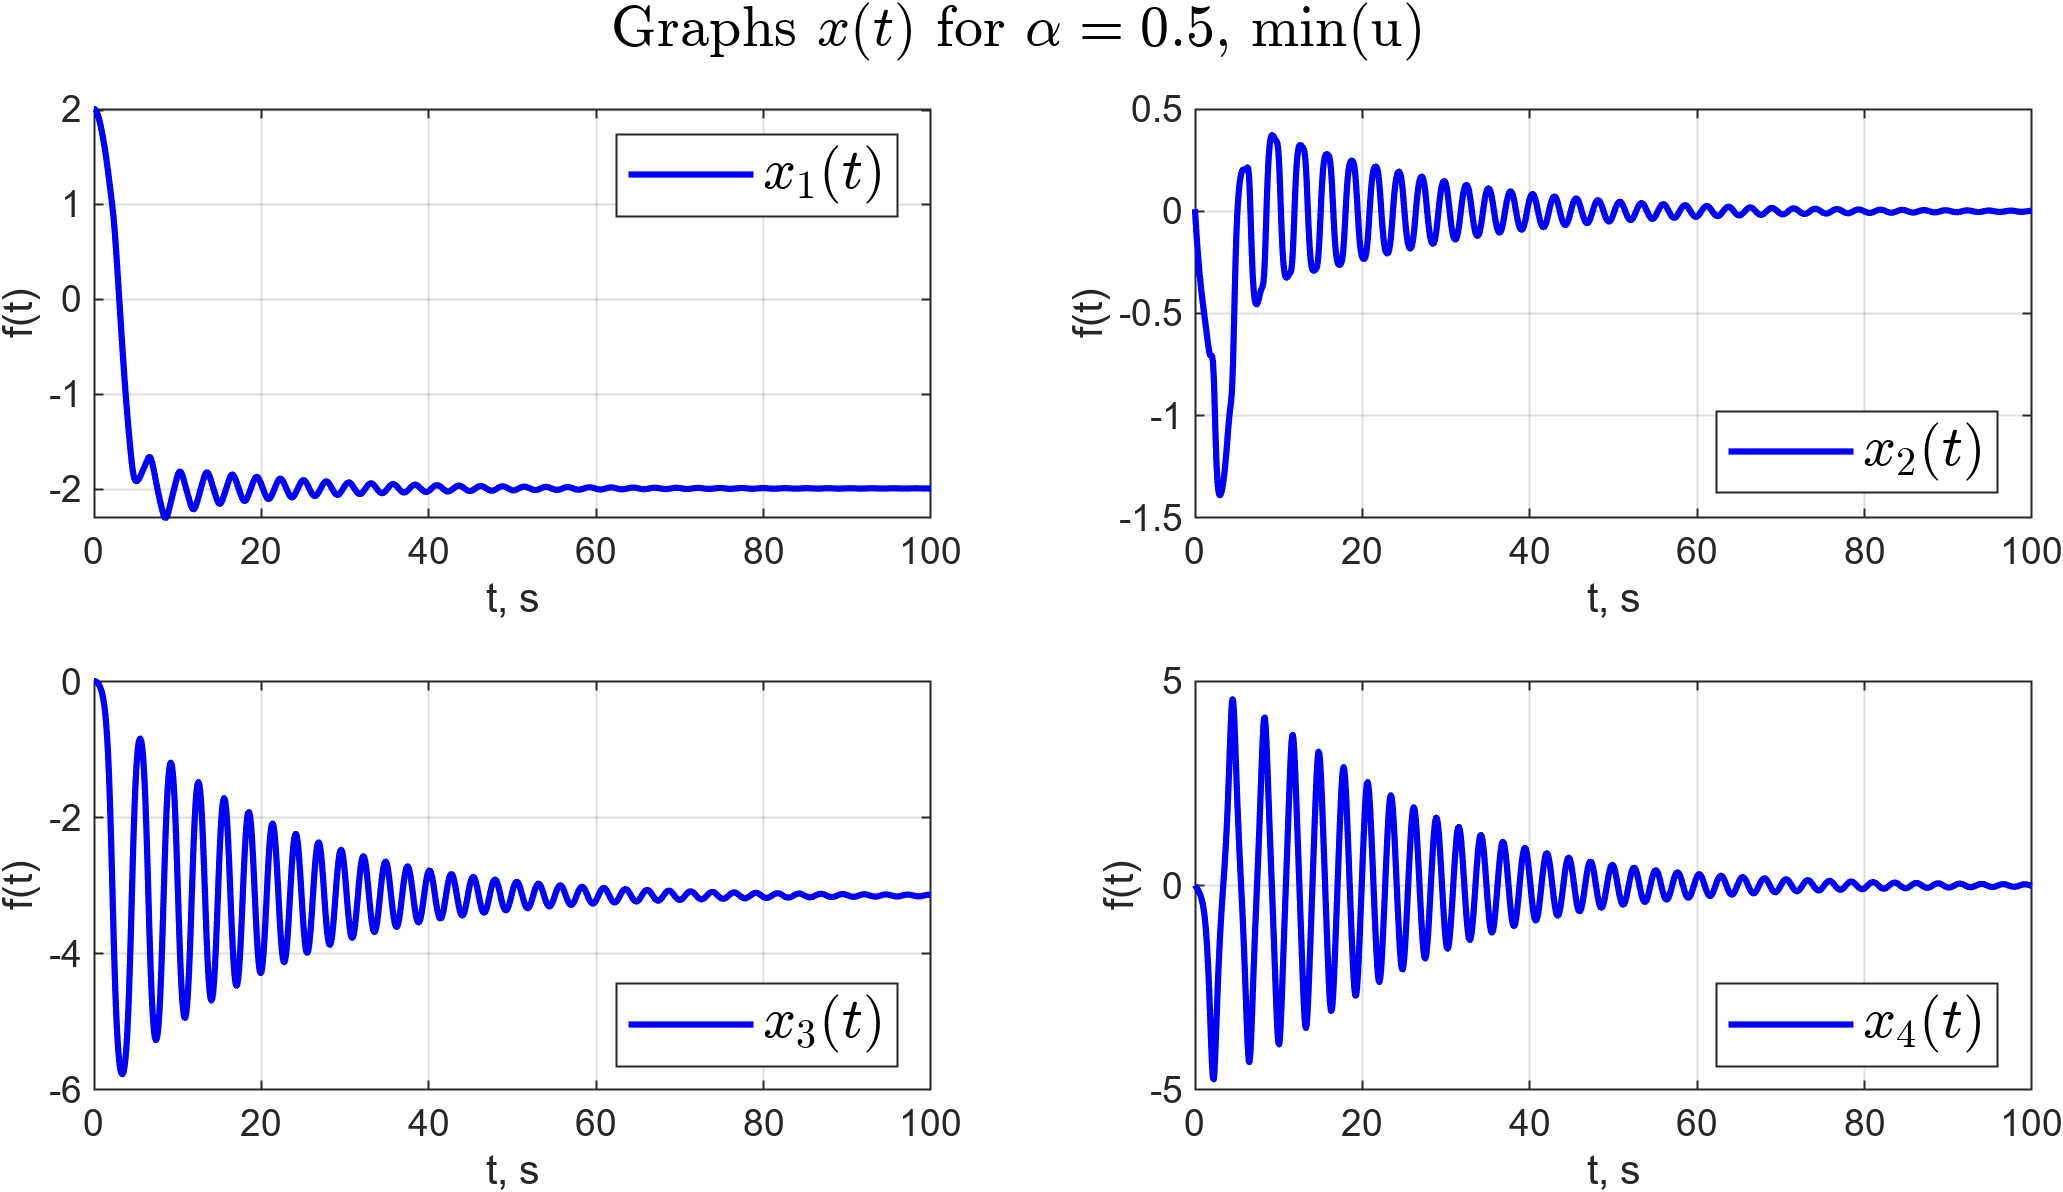
\includegraphics[width=1\linewidth]{pic/4_3_0.5_4.png}}
\caption{Графики $x(t)$, при $\alpha = 0.5$ и $x(0) = [2\, \, \,  0.01\, \, \, 0.01\, \, \, 0.01]^T$.}
\label{4_3_0.5_4}
\end{figure}

\newpage
Для $\alpha_3 = 1$ не существует решений системы неравенств при начальном значении линейной скорости $1$ м/с, поэтому возьмем новый вектор начальных условий $x(0) = [0.01\, \, \,  0.1\, \, \, 0.01\, \, \, 0.01]^T$

\begin{figure}[!h]
\center{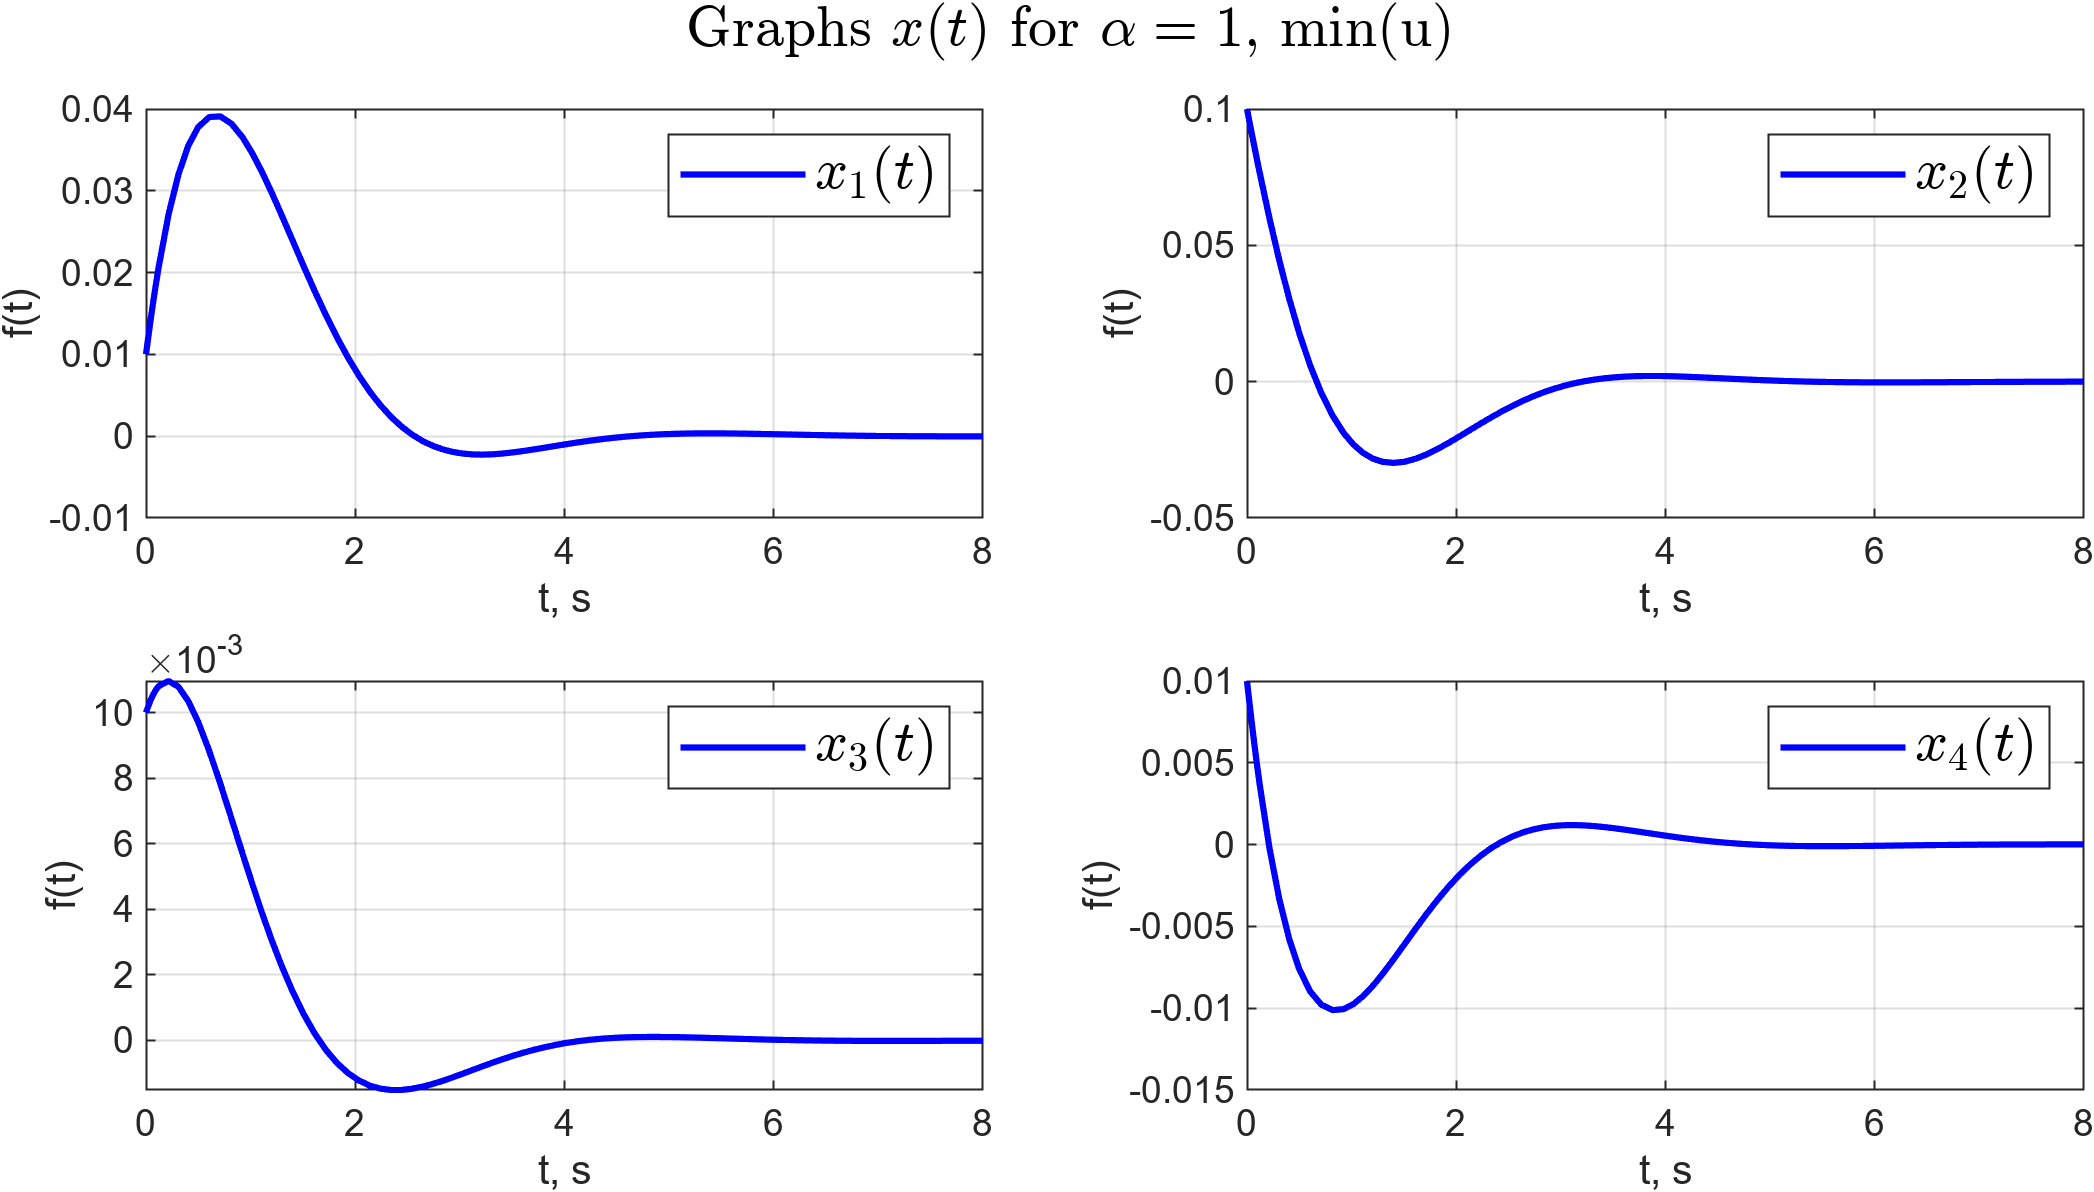
\includegraphics[width=1\linewidth]{pic/4_3_1_1.png}}
\caption{Графики $x(t)$, при $\alpha = 1$ и $x(0) = [0.01\, \, \,  0.1\, \, \, 0.01\, \, \, 0.01]^T$.}
\label{4_3_1_1}
\end{figure}

Для второго вектора начальных условий (с большим значением угловой скорости) тоже выберем вектор с меньшим значением угловой начальной скорости, потому что при $1$ рад/с для $\alpha_3 = 1$ также не удается найти решение системы, новый вектор: $x(0) = [0.01\, \, \,  0.01\, \, \, 0.01\, \, \, 0.1]^T$

\begin{figure}[!h]
\center{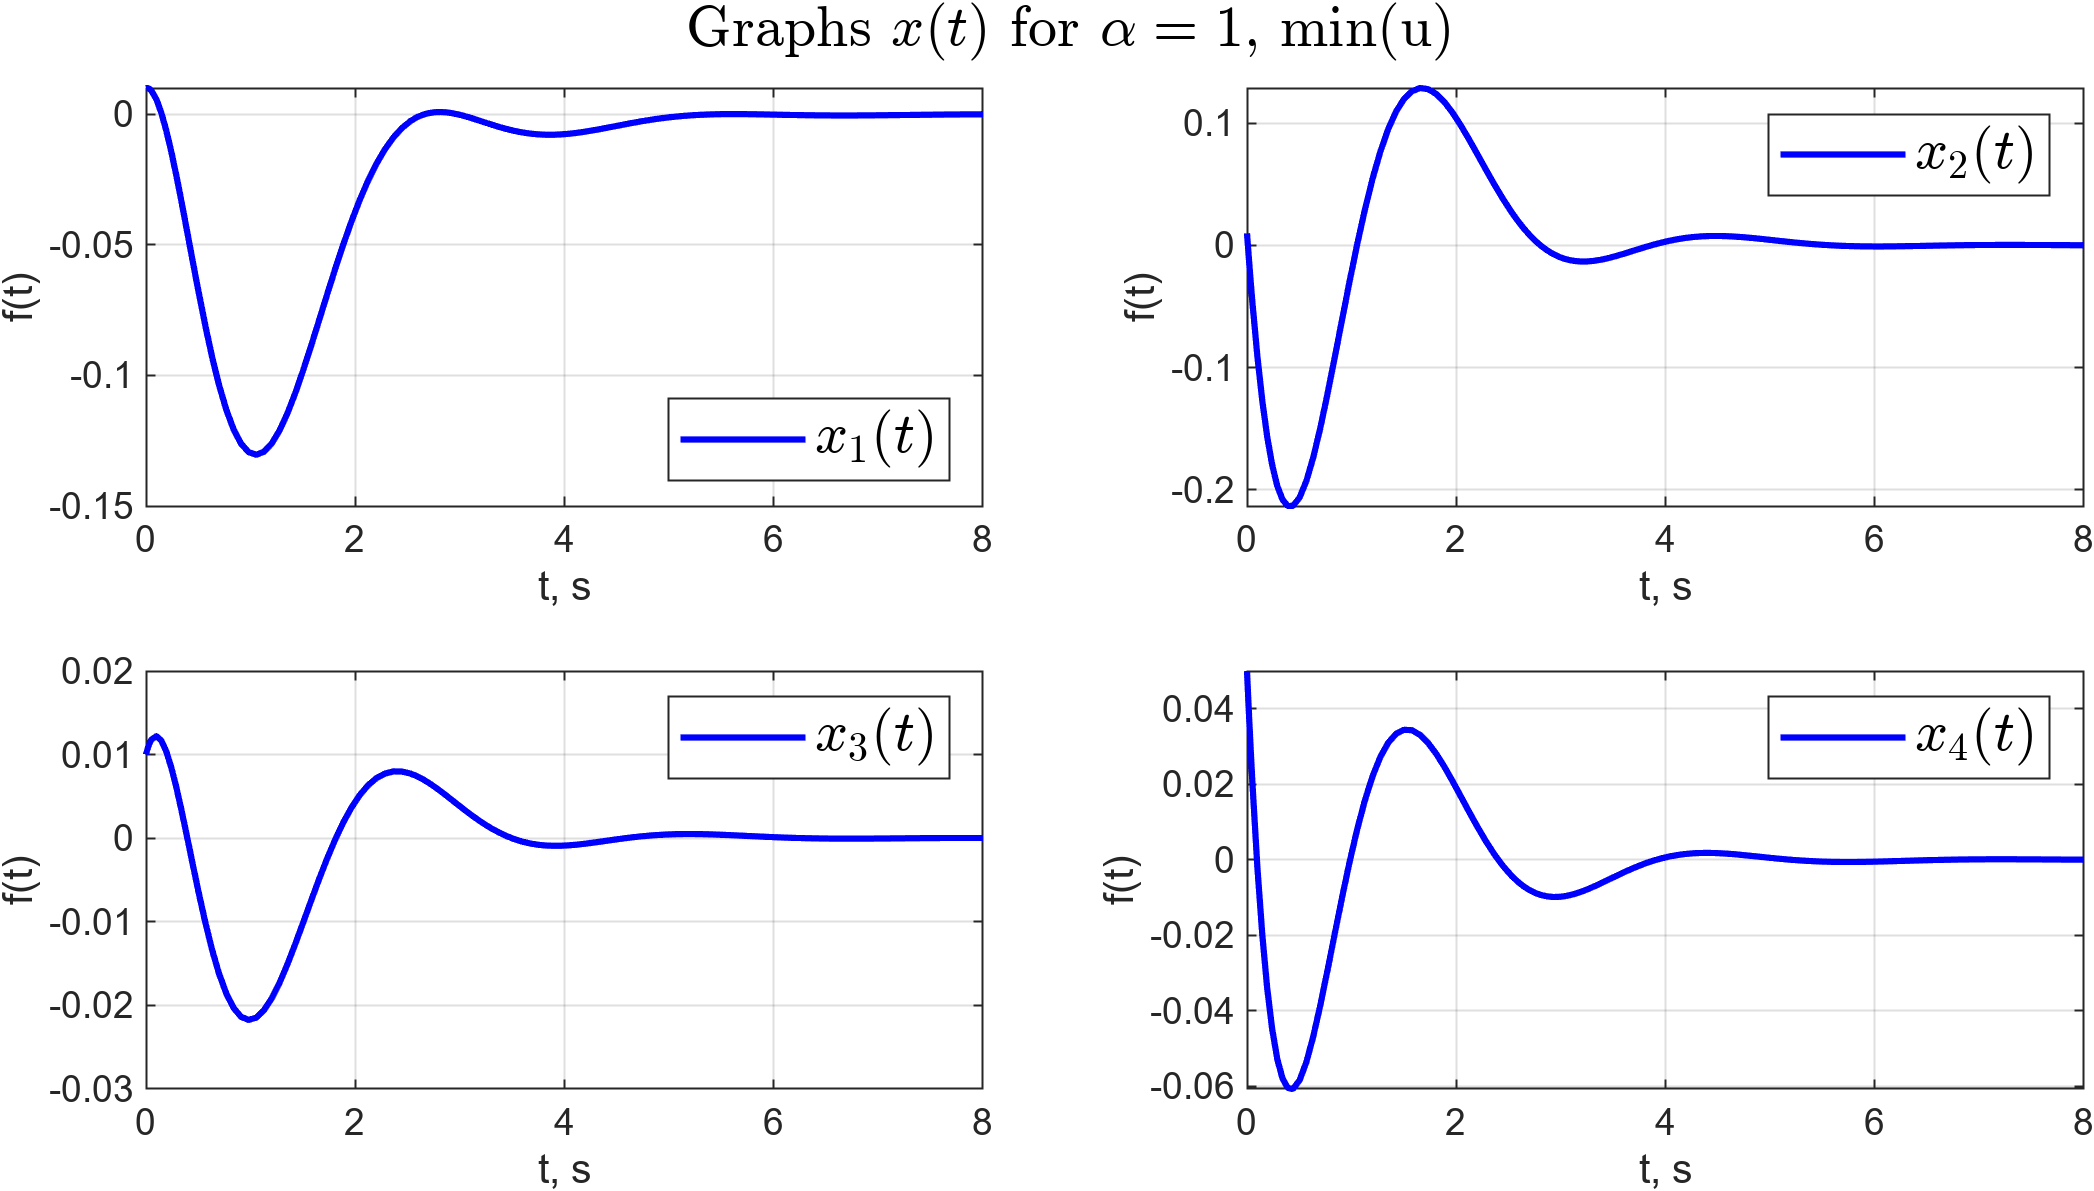
\includegraphics[width=1\linewidth]{pic/4_3_1_2.png}}
\caption{Графики $x(t)$, при $\alpha = 1$ и $x(0) = [0.01\, \, \,  0.01\, \, \, 0.01\, \, \, 0.1]^T$.}
\label{4_3_1_2}
\end{figure}


\begin{figure}[!h]
\center{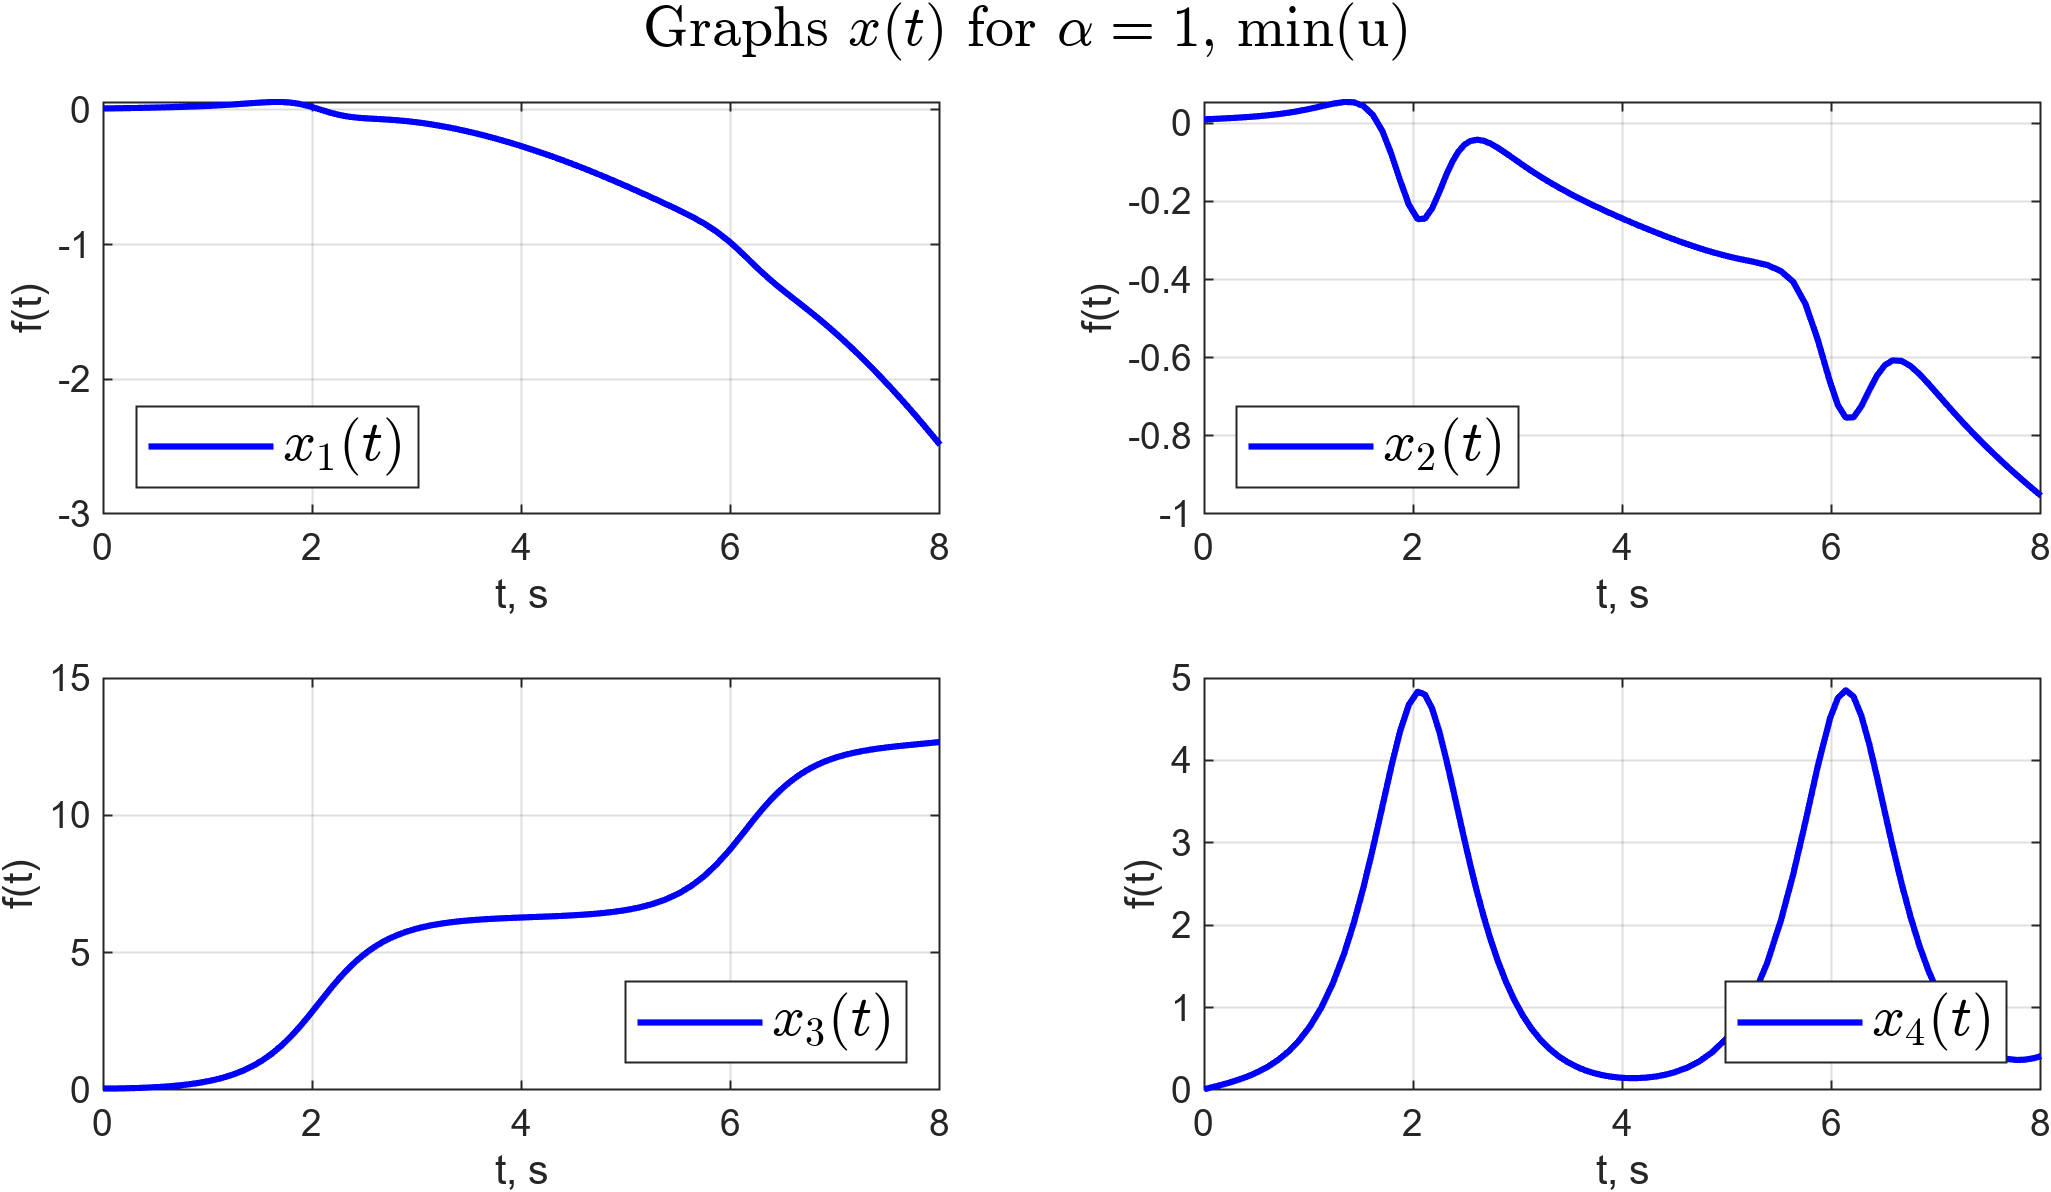
\includegraphics[width=1\linewidth]{pic/4_3_1_3.png}}
\caption{Графики $x(t)$, при $\alpha = 1$ и $x(0) = [0.01\, \, \,  0.01\, \, \, \pi / 60\, \, \, 0.01]^T$.}
\label{4_3_1_3}
\end{figure}


\begin{figure}[!h]
\center{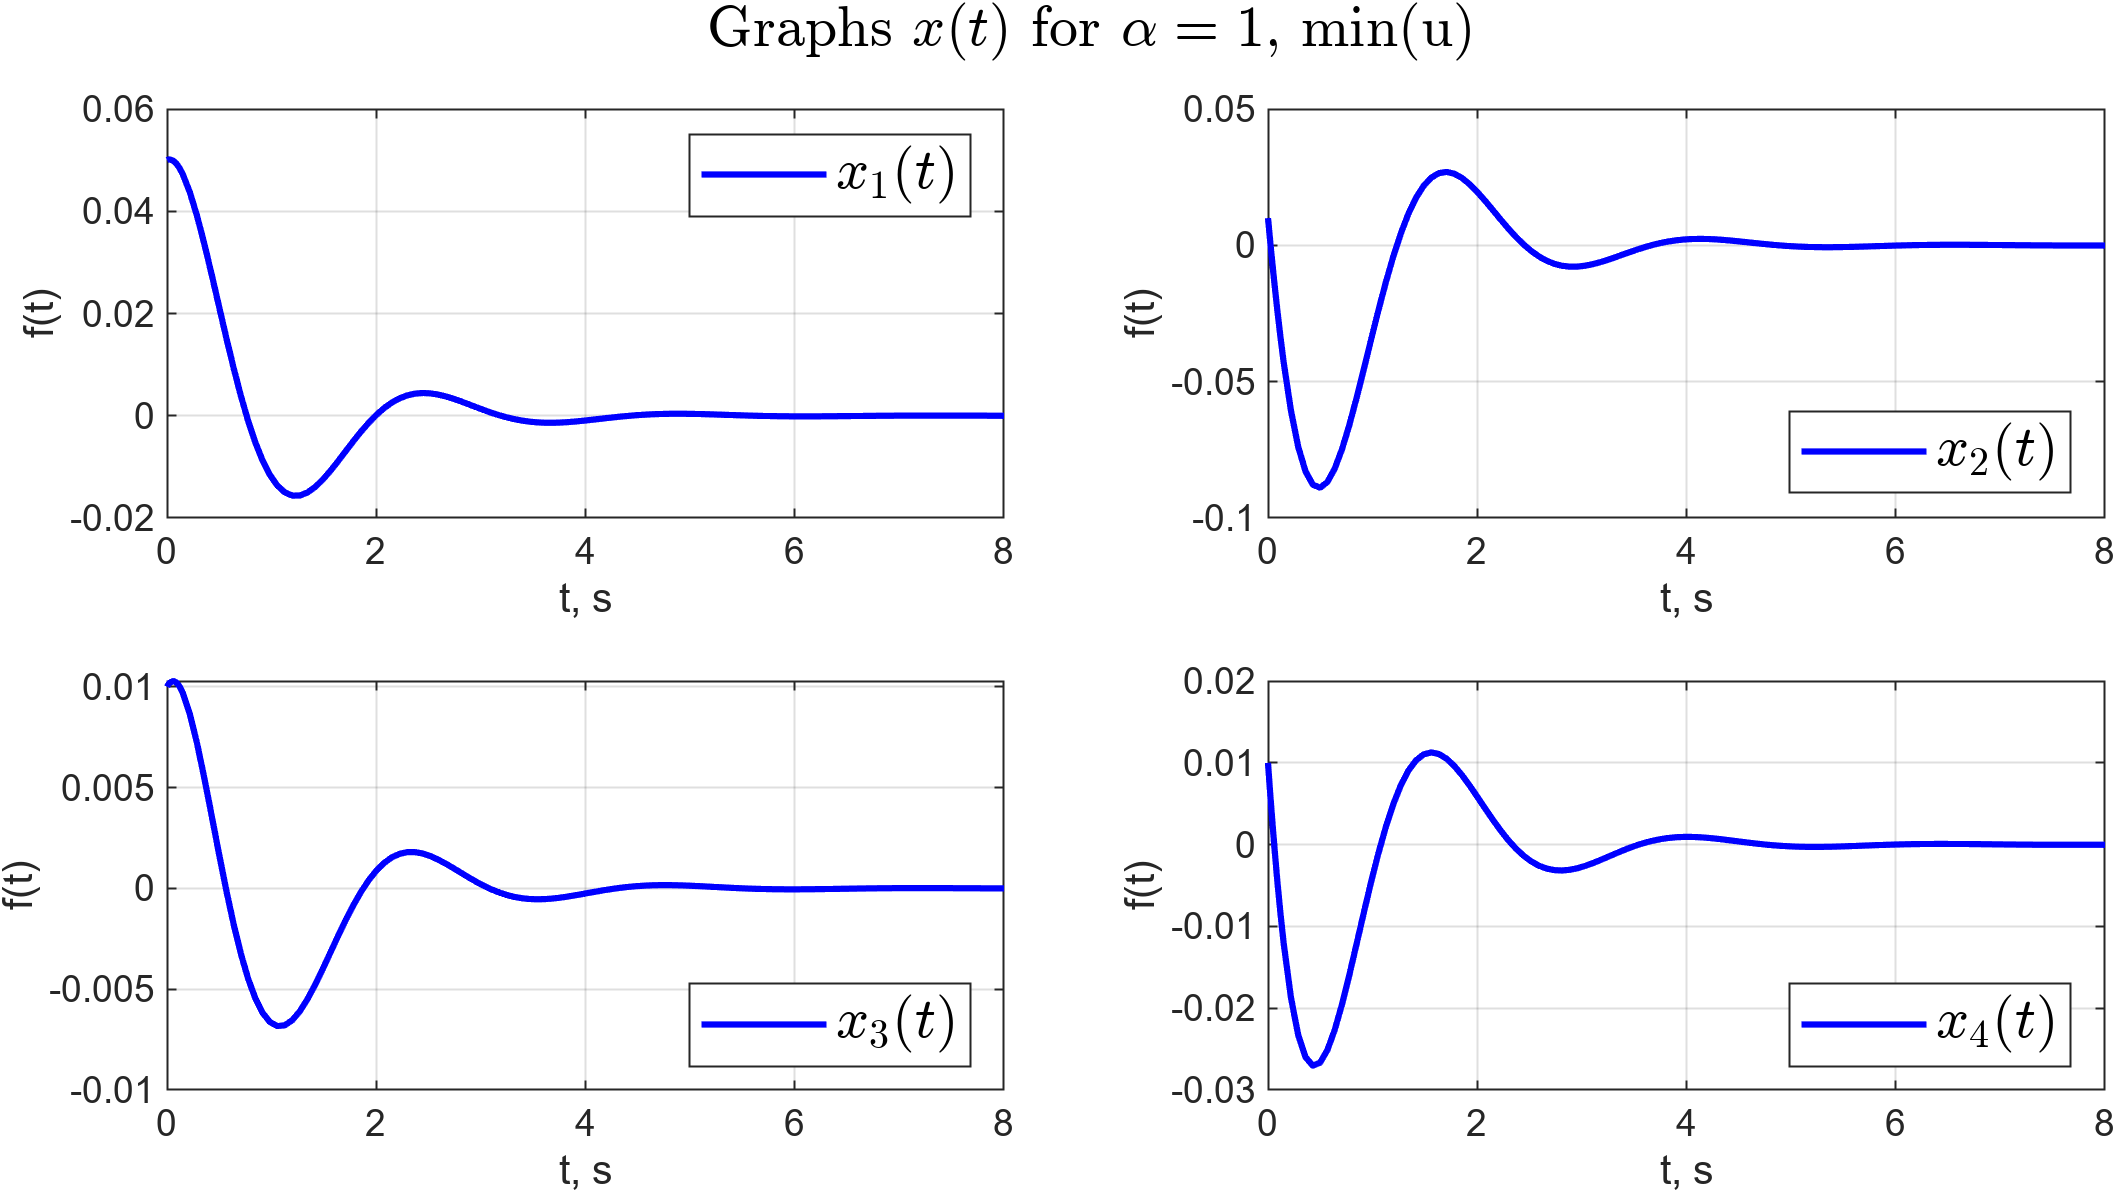
\includegraphics[width=1\linewidth]{pic/4_3_1_4.png}}
\caption{Графики $x(t)$, при $\alpha = 1$ и $x(0) = [0.05\, \, \,  0.01\, \, \, 0.01\, \, \, 0.01]^T$.}
\label{4_3_1_4}
\end{figure}

\newpage
С ростом значения $\alpha$ существенно сужалась область допустимых начальных условий, при которых система матричных неравенств имеет решение.

\section{Исследование регулятора по состоянию с ограничением на управление}

Исследуем влияние параметра $\alpha$ на максимальное отклонение маятника от вертикали, максимальное горизонтальное смещение тележки и максимальное значение сигнала при управлении нелинейной системой (\ref{1_model_full}), результаты представим в таблице \ref{4_tab_4}


\begin{table}[h]
\centering
\caption{Результаты моделирования при разных значениях параметра $\alpha$.}
\label{4_tab_4}
\begin{tabular}{ccccc}
\toprule
$\alpha$ & $\max |\varphi|$ & $\max |a|$ & $\max |u|$ \\
\midrule
0.1  &  0.012  &  0.51  &  45 \\
0.5  &  0.01  &  0.09  &   79 \\
1 &  0.01  &  0.05  &  138  \\
2  &  13946  &  2879 &   46 \\
\bottomrule
\end{tabular}
\end{table}

В таблице \ref{4_tab_4} для $\alpha=2$ указаны значения, полученные в результате моделирования, истинные значения параметров стремятся к бесконечности с ростом времени моделирования.

До значения $\alpha=2$ (не включительно) мы видим снижение таких параметров как максимальное отклонение маятника от вертикали и максимальное горизонтальное смещение тележки. Также с ростом $\alpha$ мы наблюдаем рост максимального значения управляющего сигнала. При $\alpha=2$ регулятор не обеспечивает стабилизацию системы, поэтому мы получаем большие значения угла, координаты. Результаты моделирования представлены на рисунках \ref{4_4_x_01}-\ref{4_4_u_2}.

% alpha = 0.1
\begin{figure}[!h]
	\center{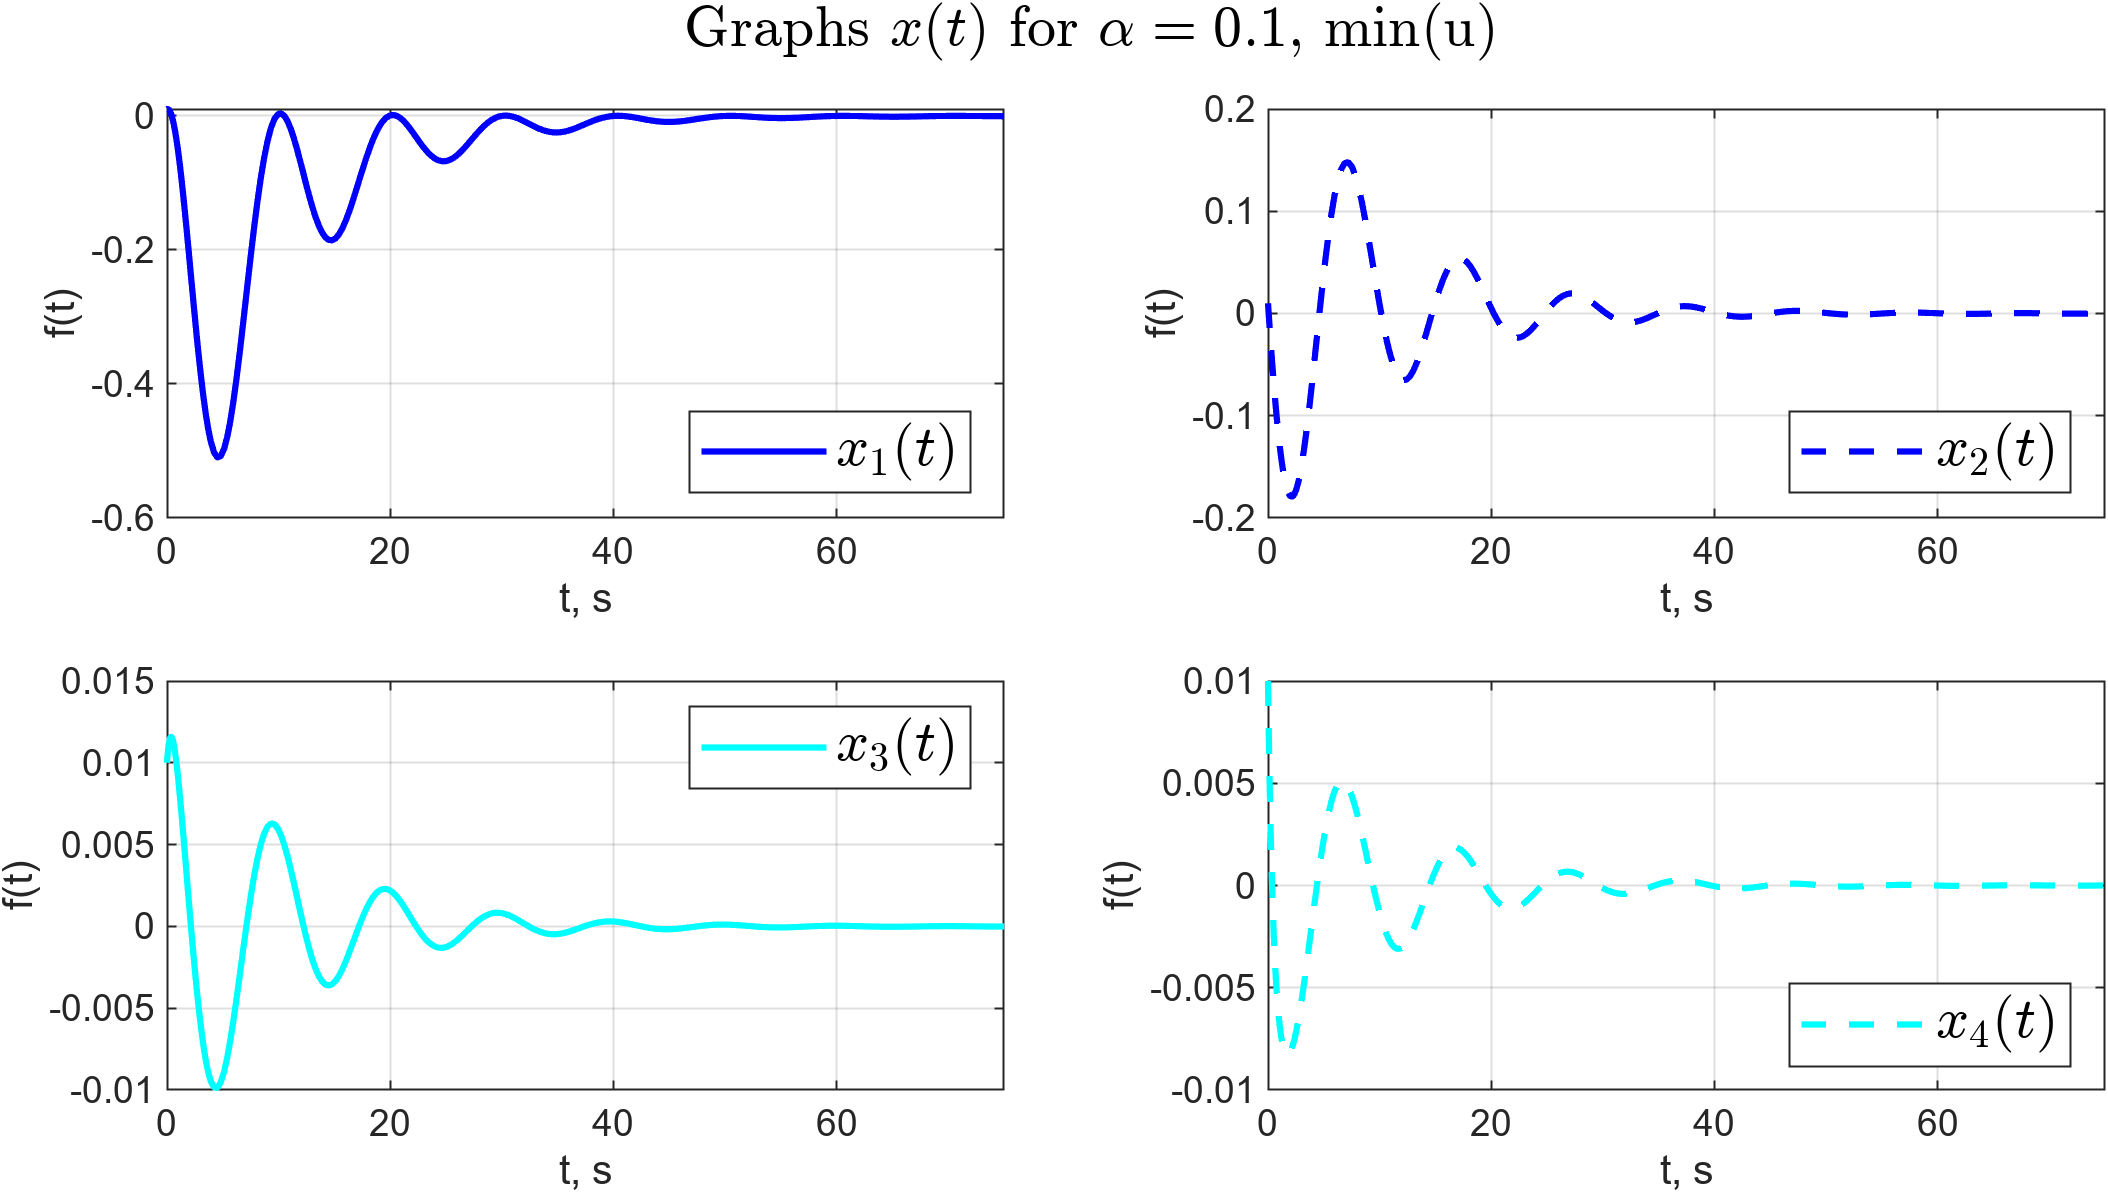
\includegraphics[width=1\linewidth]{pic_fix/4_4_x_01.png}}
	\caption{Графики вектора состояния системы при $\alpha = 0.1$.}
	\label{4_4_x_01}
\end{figure}

\begin{figure}[!h]
	\center{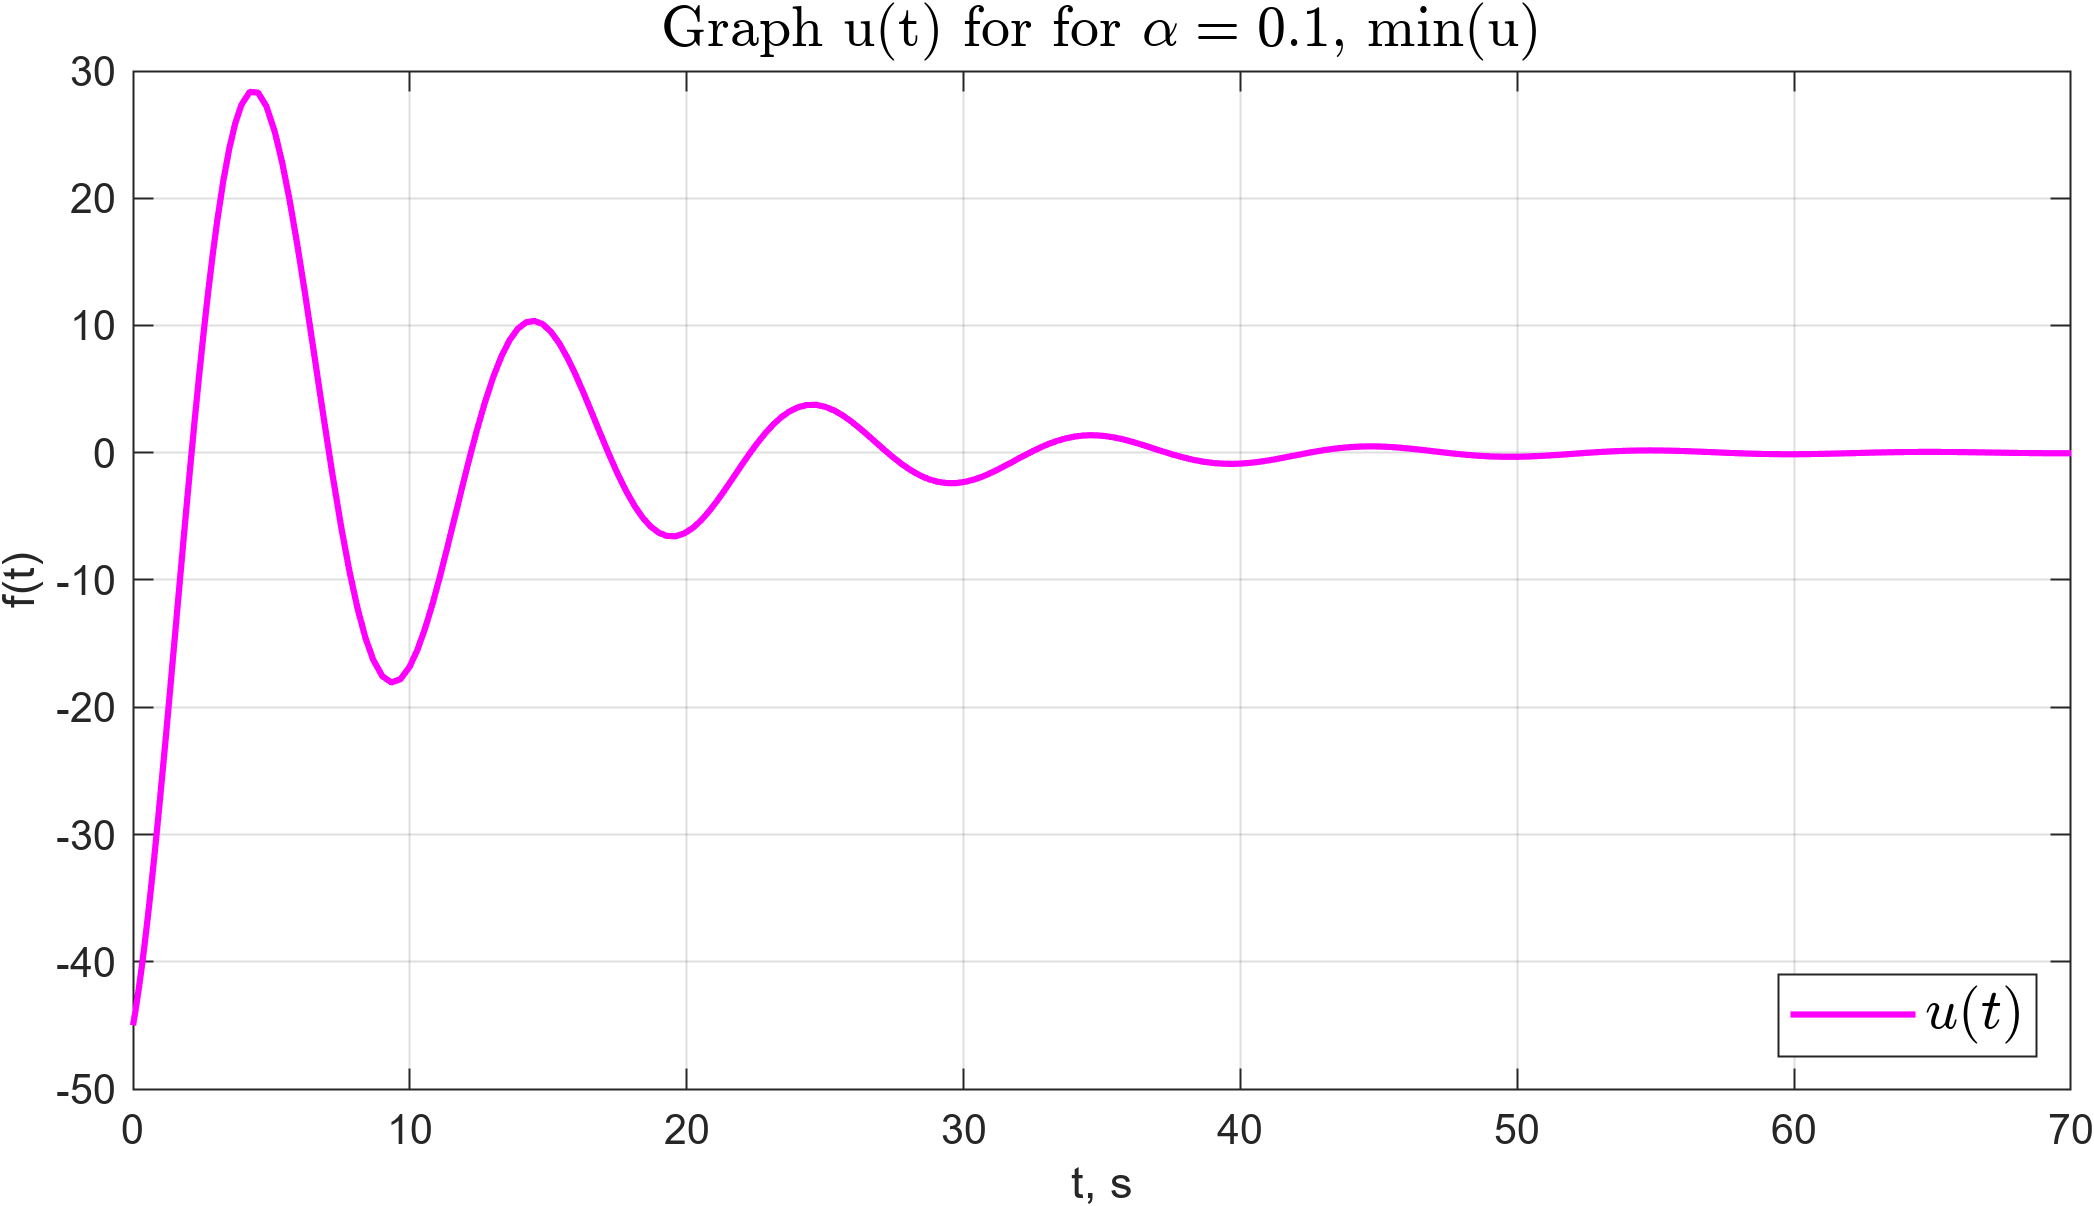
\includegraphics[width=1\linewidth]{pic_fix/4_4_u_01.png}}
	\caption{График $u(t)$ при $\alpha = 0.1$.}
	\label{4_4_u_01}
\end{figure}


% alpha = 0.5
\begin{figure}[!h]
	\center{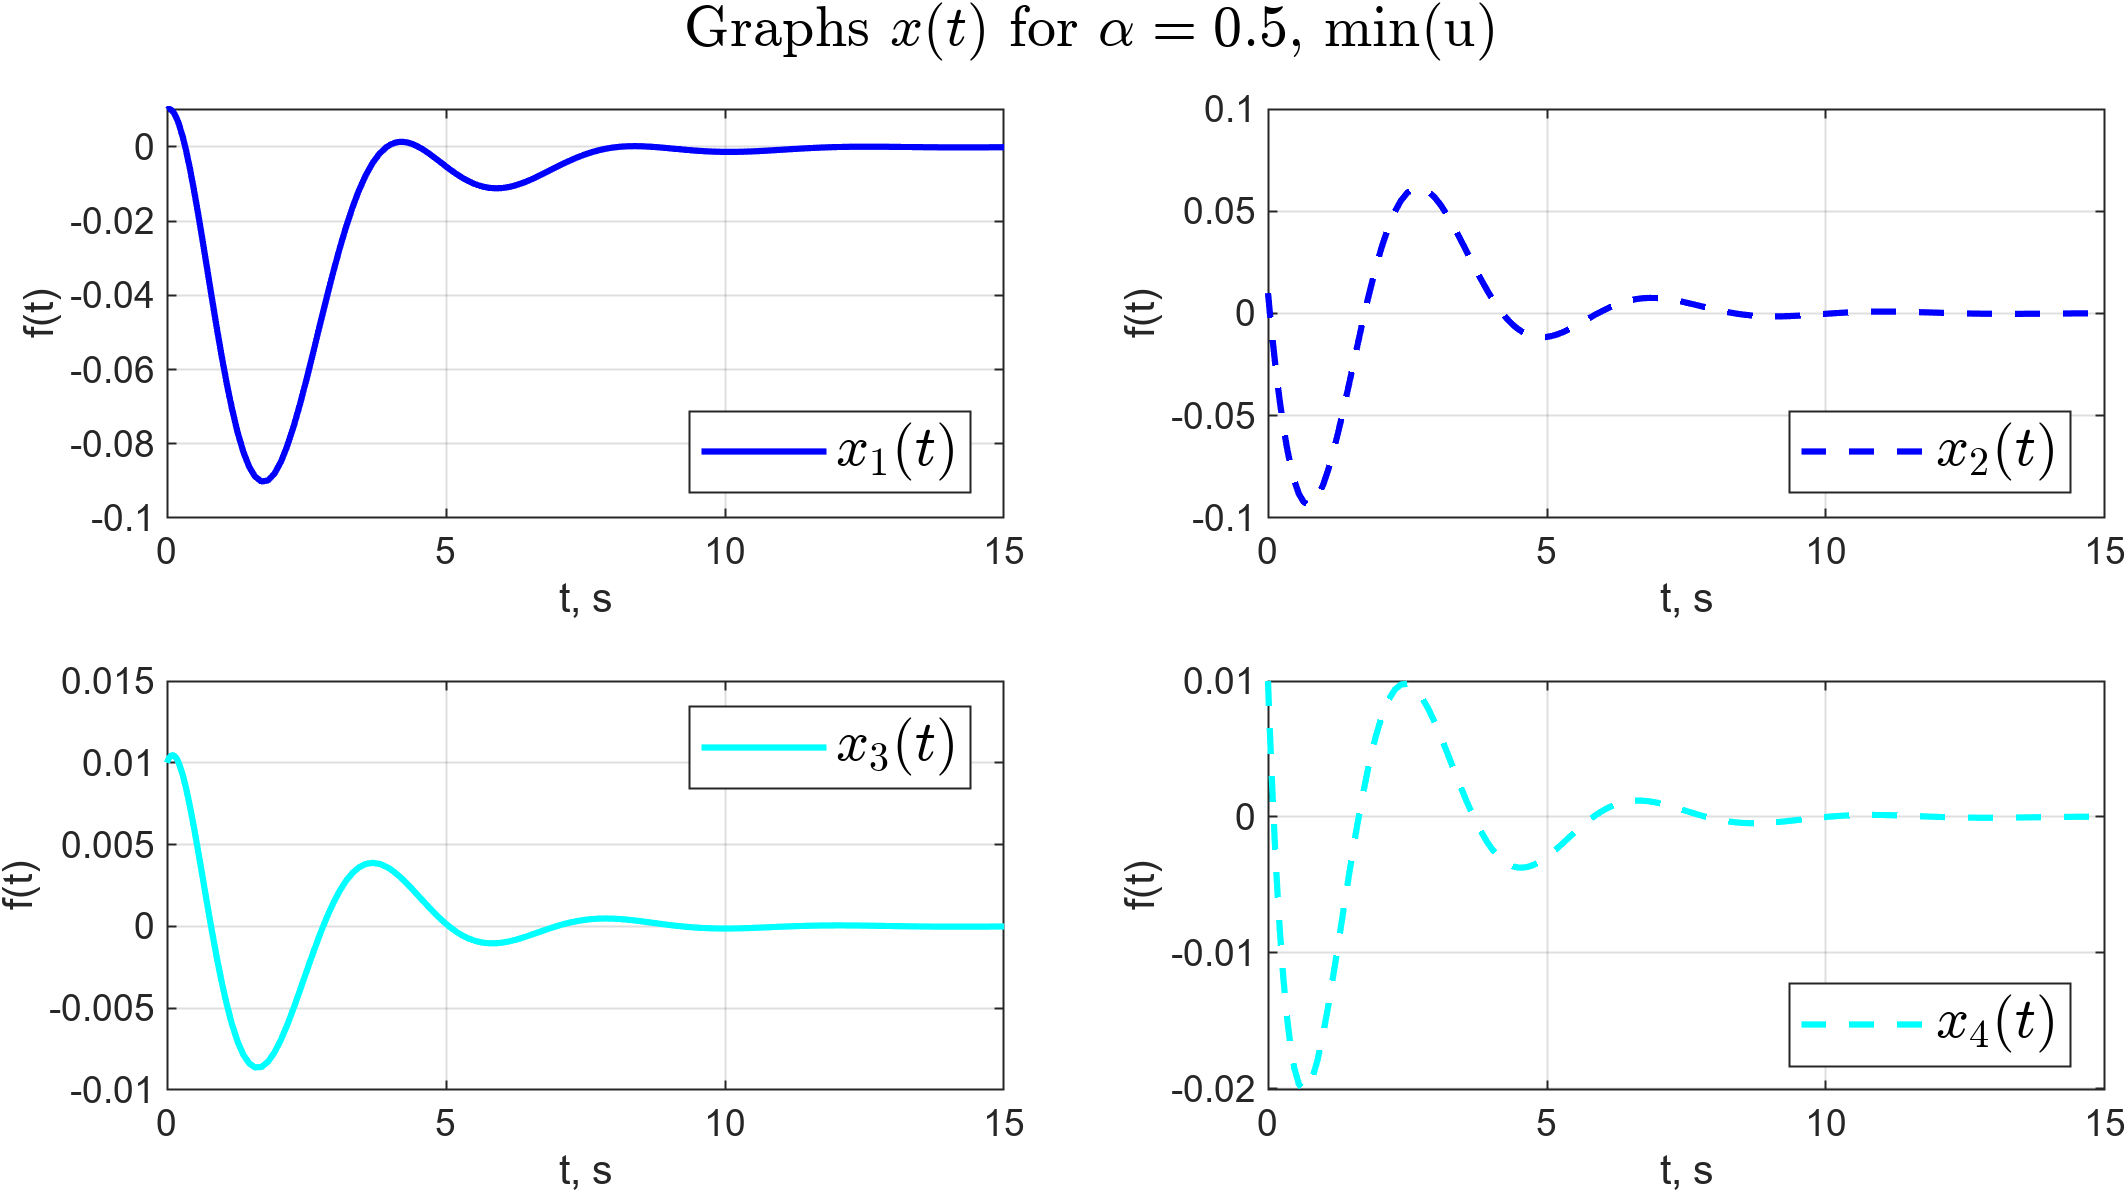
\includegraphics[width=1\linewidth]{pic_fix/4_4_x_05.png}}
	\caption{Графики вектора состояния системы при $\alpha = 0.5$.}
	\label{4_4_x_05}
\end{figure}

\begin{figure}[!h]
	\center{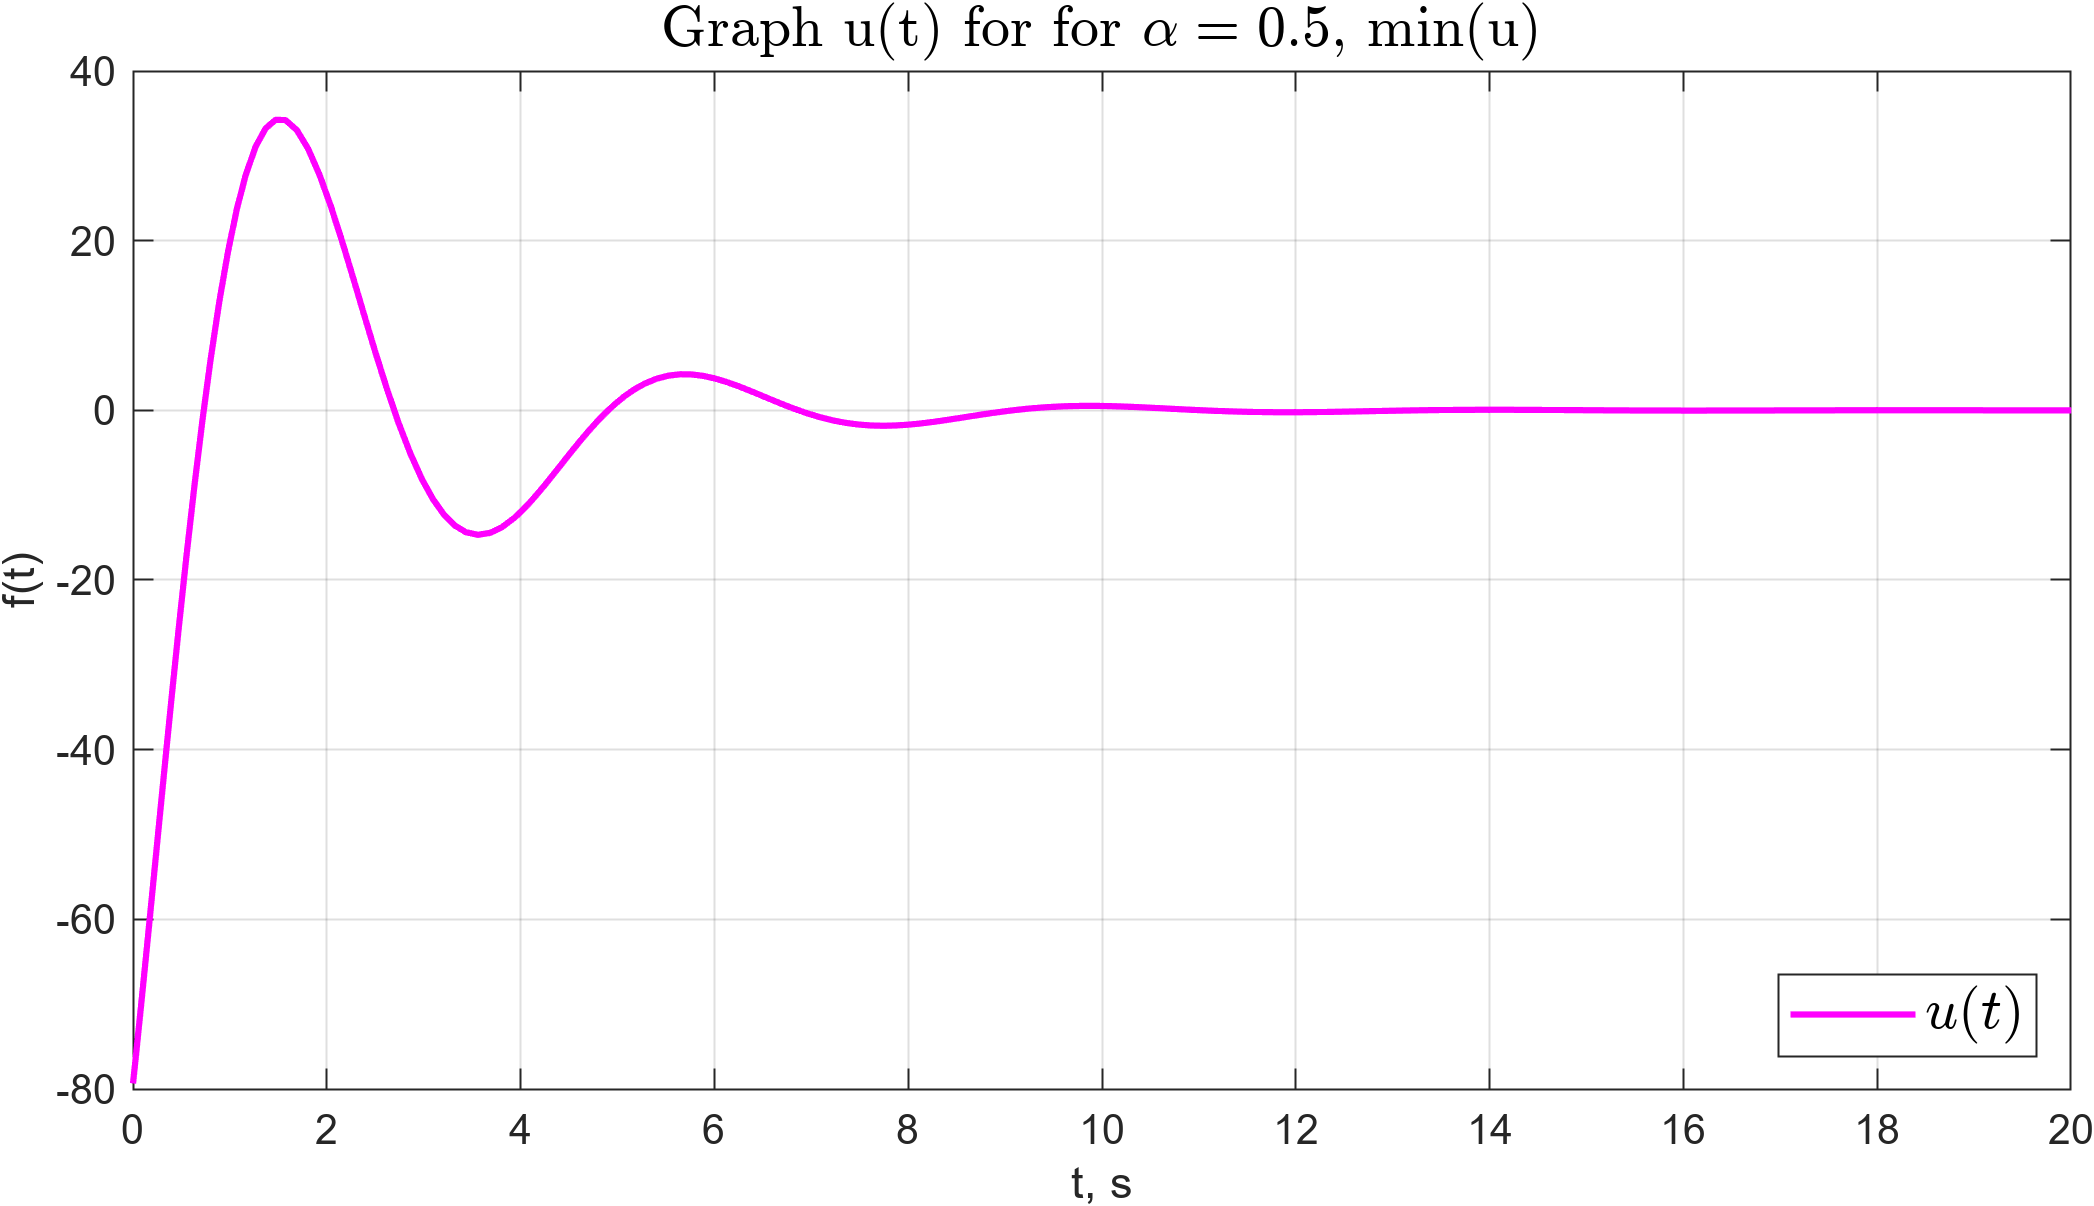
\includegraphics[width=1\linewidth]{pic_fix/4_4_u_05.png}}
	\caption{График $u(t)$ при $\alpha = 0.5$.}
	\label{4_4_u_05}
\end{figure}



% alpha = 1
\begin{figure}[!h]
	\center{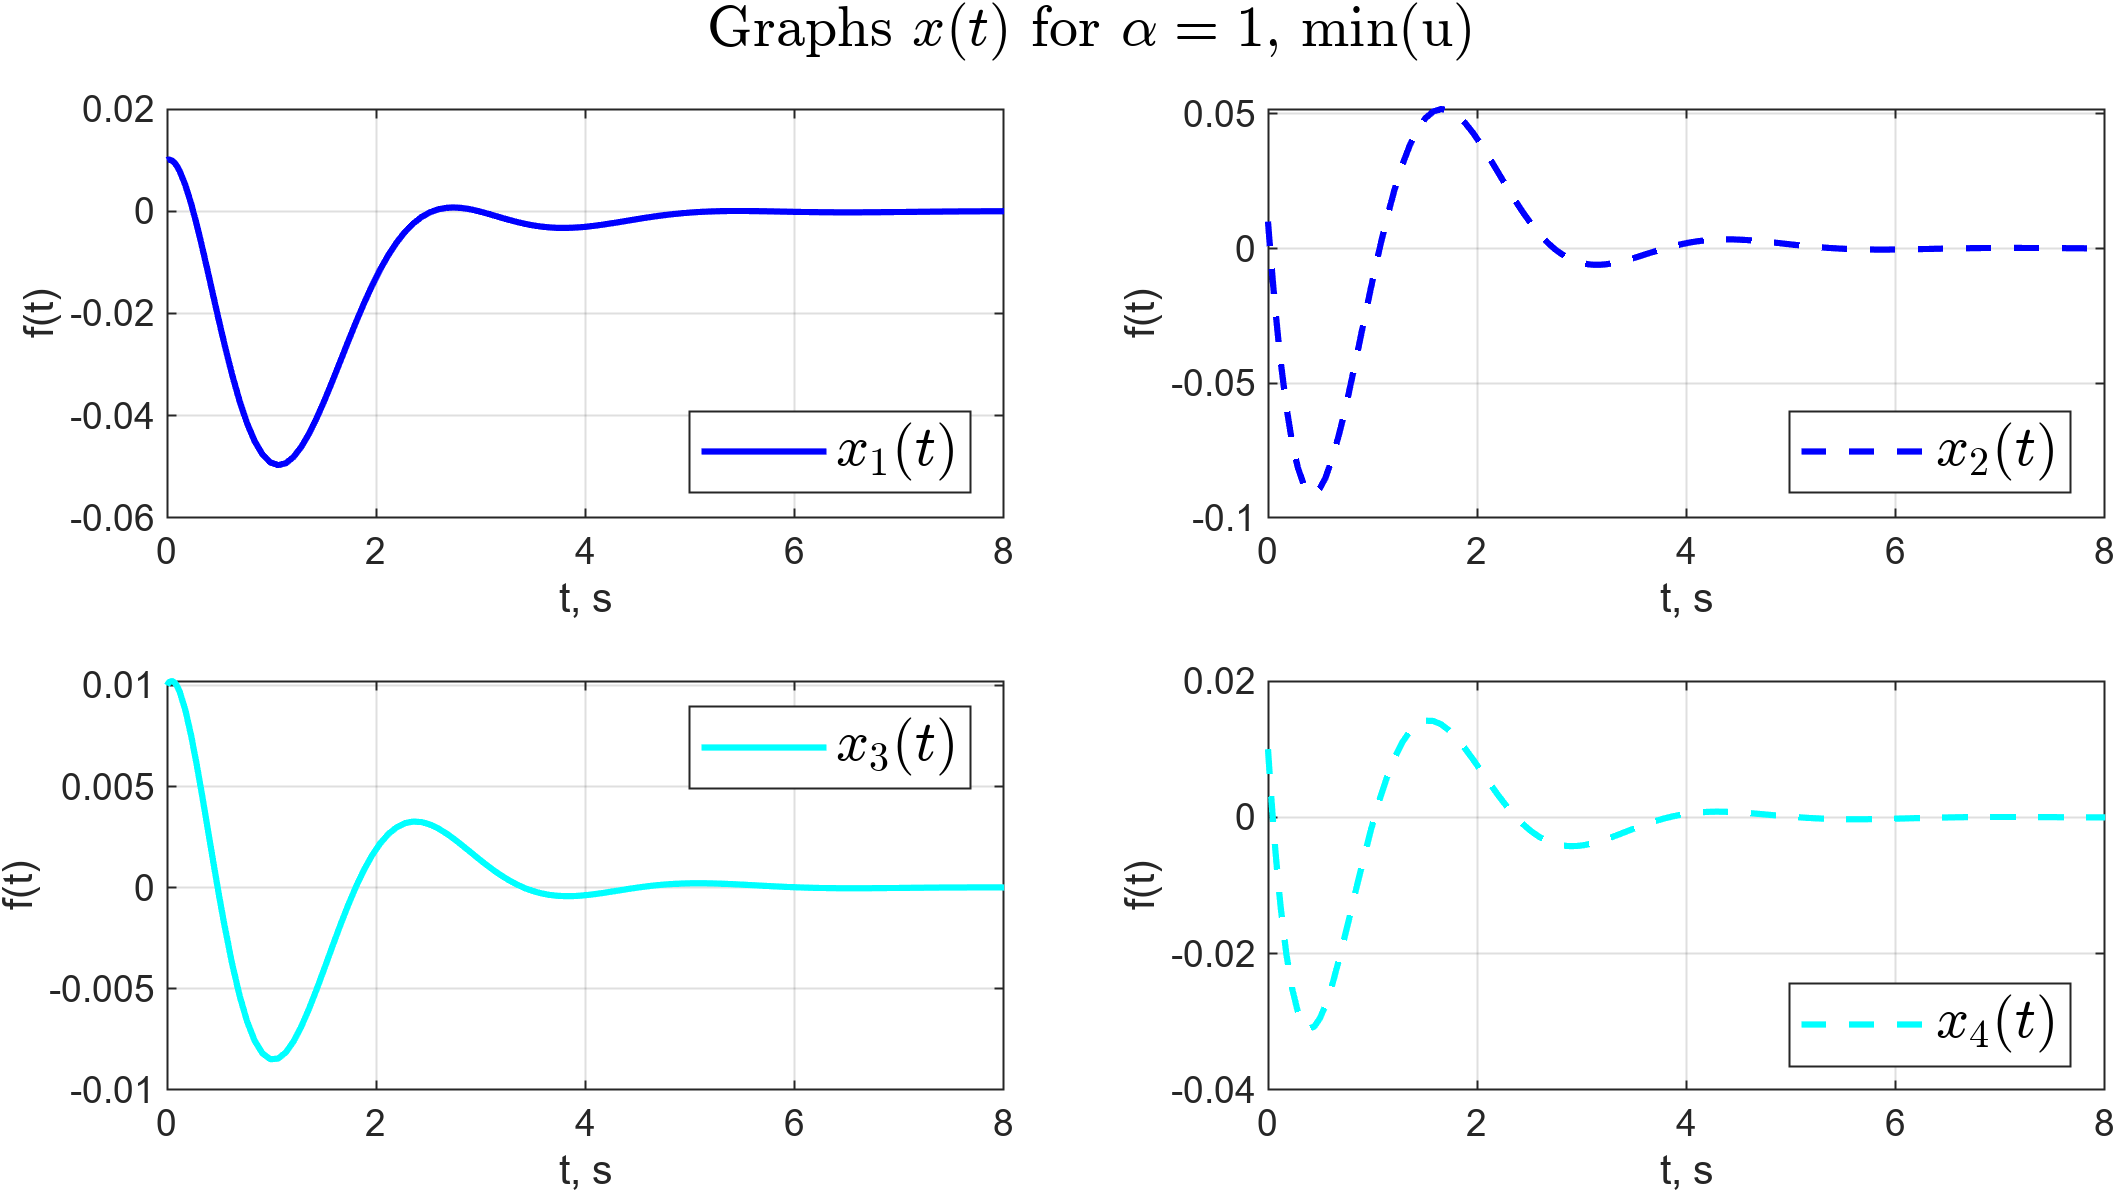
\includegraphics[width=1\linewidth]{pic_fix/4_4_x_1.png}}
	\caption{Графики вектора состояния системы при $\alpha = 1$.}
	\label{4_4_x_1}
\end{figure}

\begin{figure}[!h]
	\center{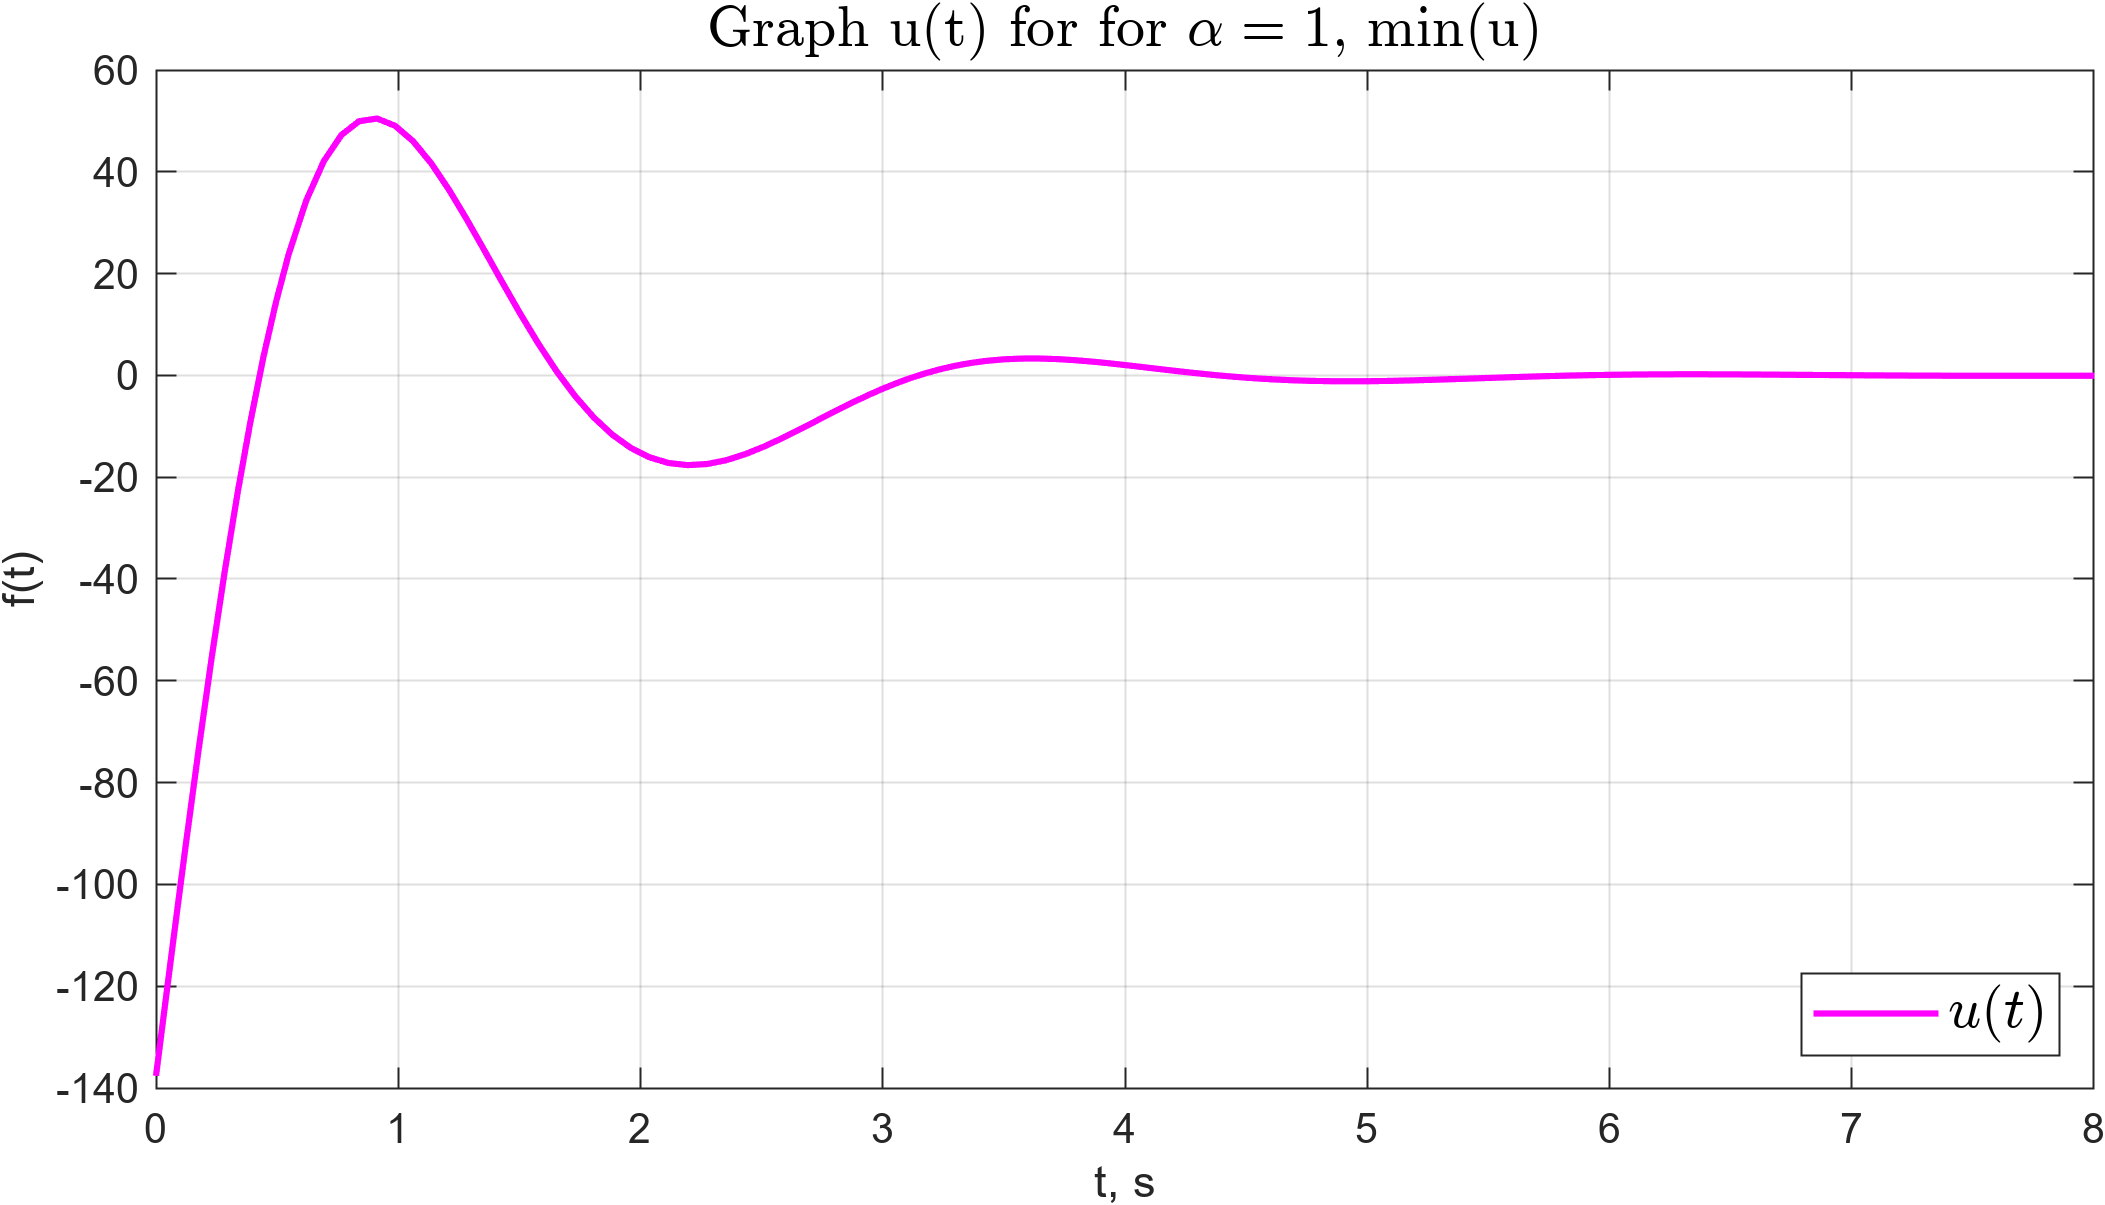
\includegraphics[width=1\linewidth]{pic_fix/4_4_u_1.png}}
	\caption{График $u(t)$ при $\alpha = 1$.}
	\label{4_4_u_1}
\end{figure}


% alpha = 2
\begin{figure}[!h]
	\center{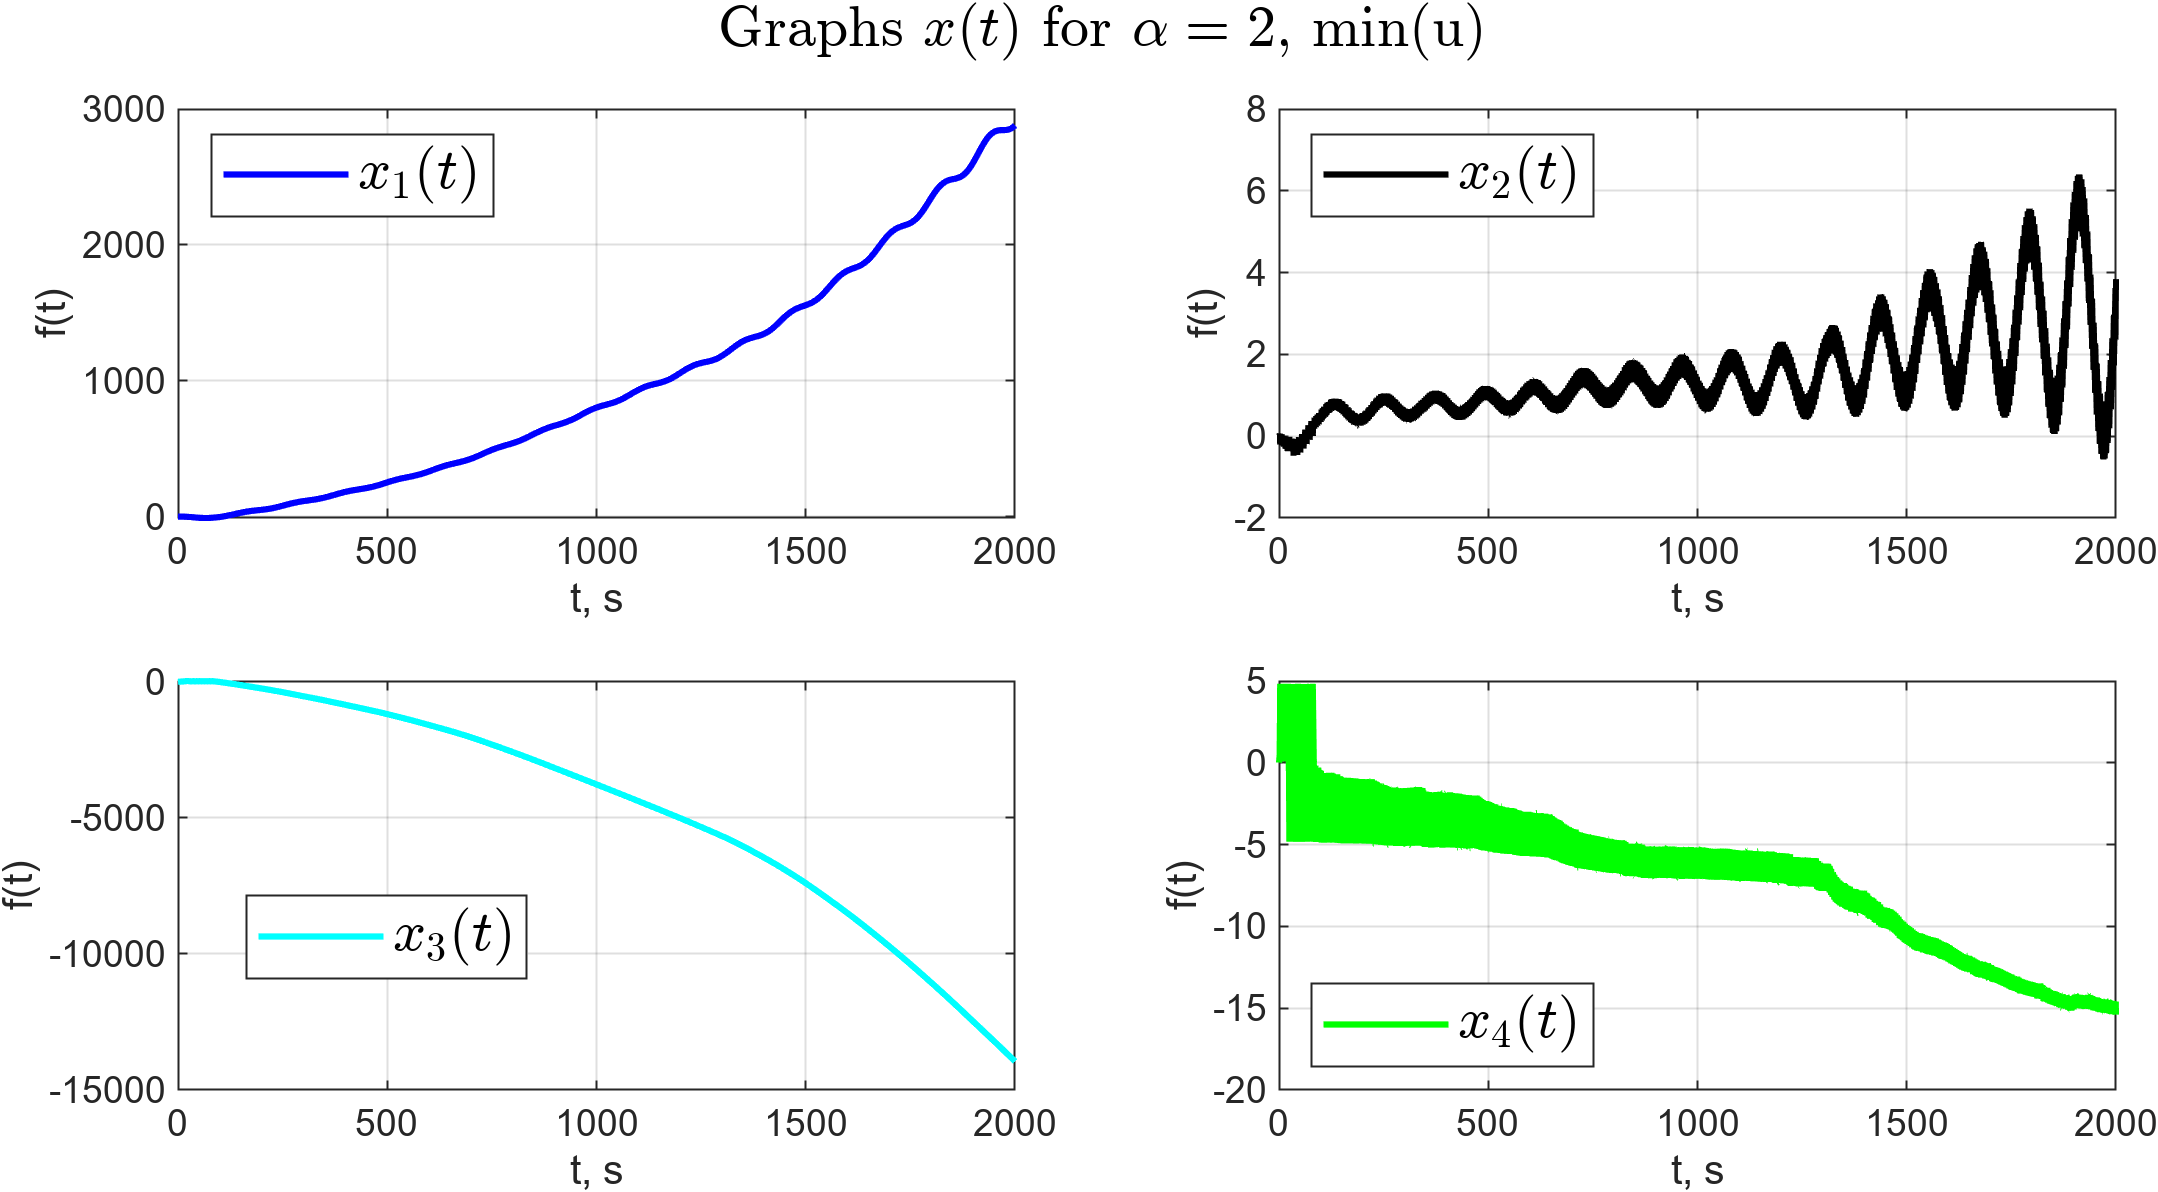
\includegraphics[width=1\linewidth]{pic_fix/4_4_x_2.png}}
	\caption{Графики вектора состояния системы при $\alpha = 2$.}
	\label{4_4_x_2}
\end{figure}

\begin{figure}[!h]
	\center{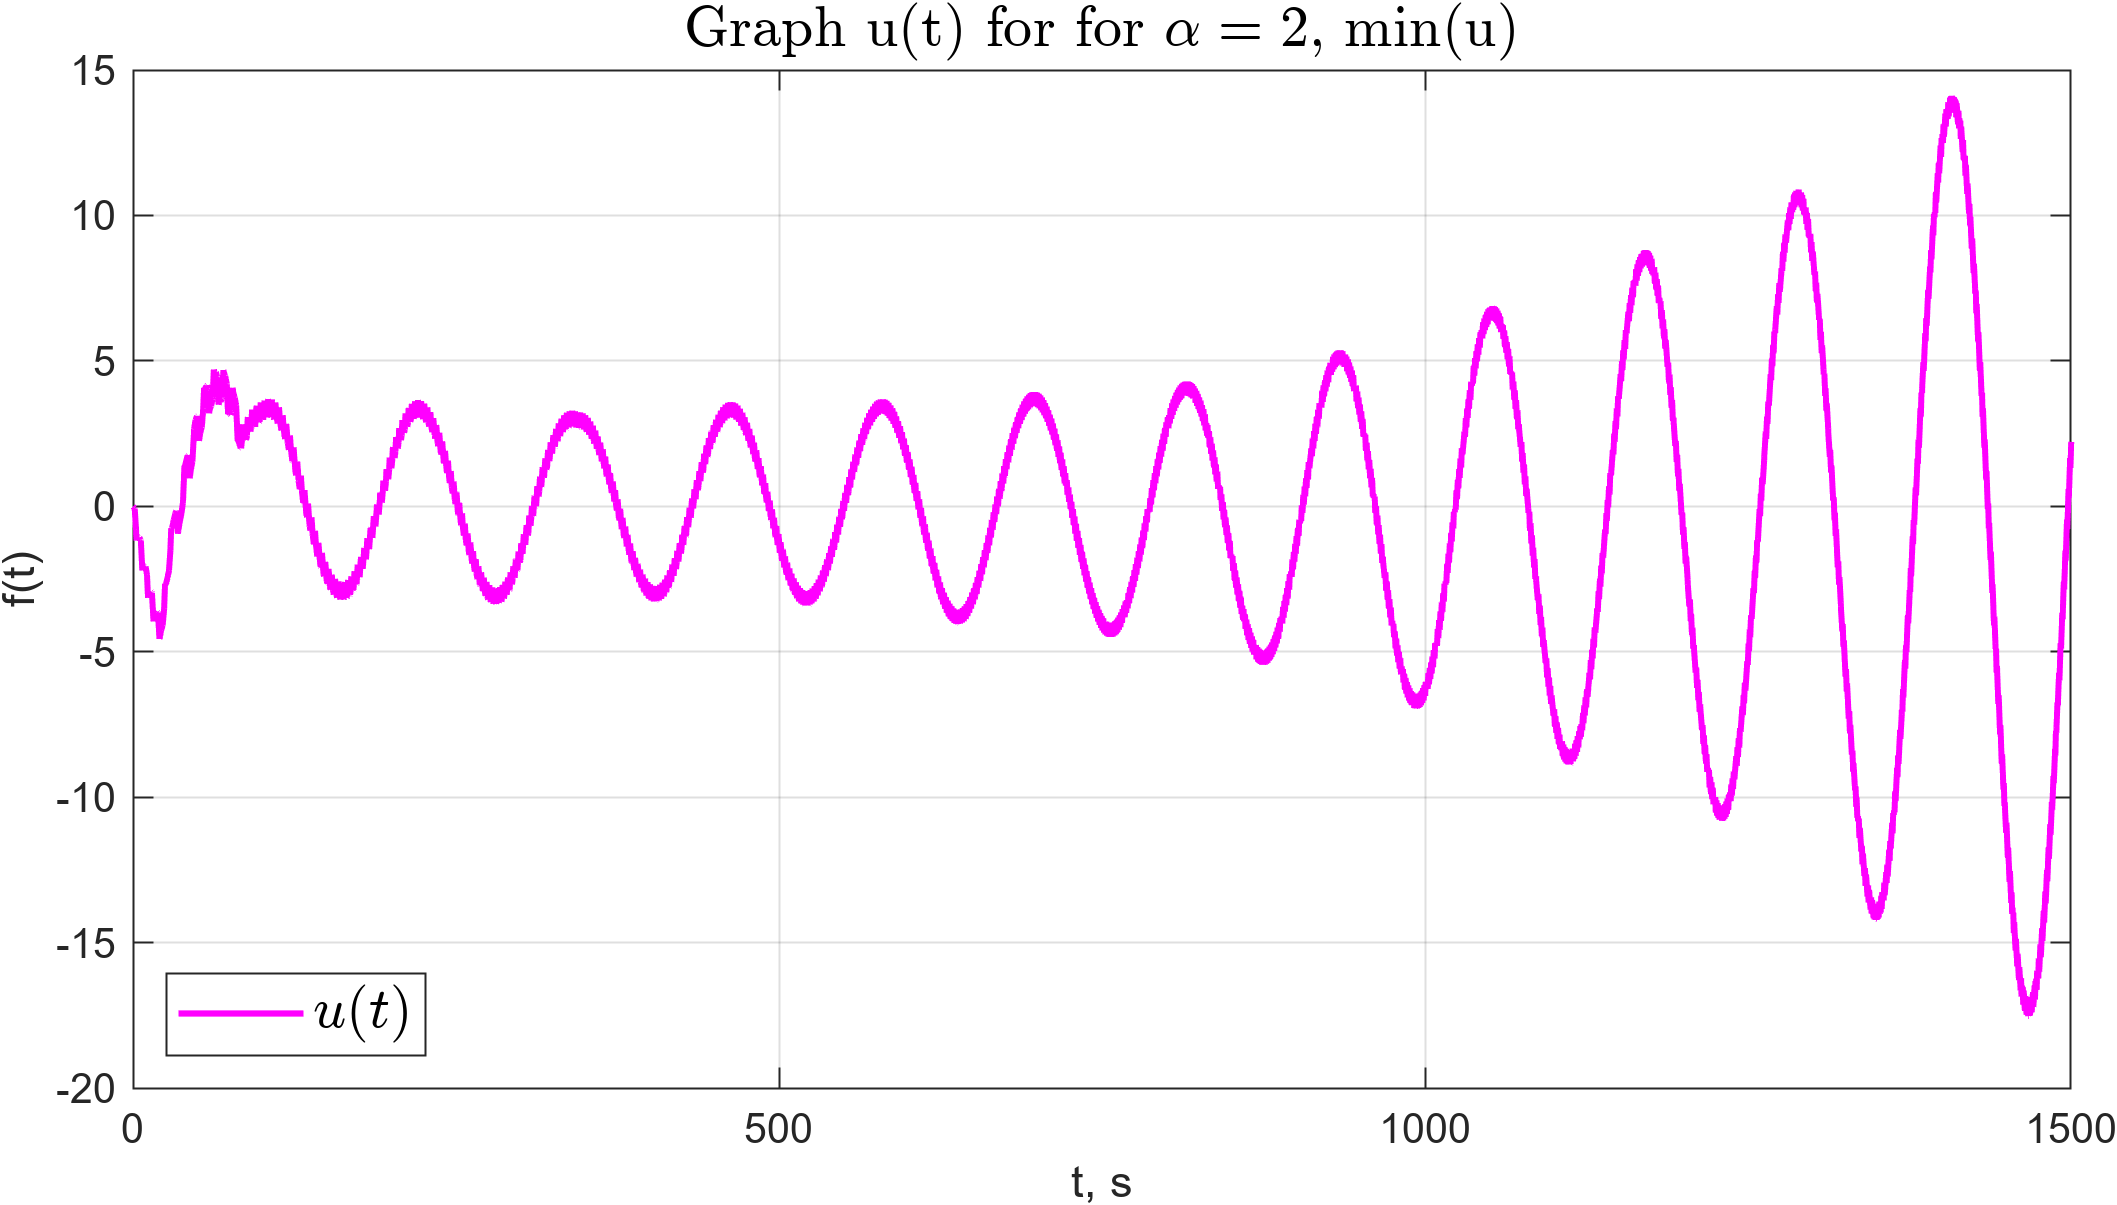
\includegraphics[width=1\linewidth]{pic_fix/4_4_u_2.png}}
	\caption{График $u(t)$ при $\alpha = 2$.}
	\label{4_4_u_2}
\end{figure}



\section{Синтез наблюдателя}
С помощью решения линейного матричного неравенства Ляпунова для экспоненциальной устойчивости произведем расчет наблюдателя полной размерности
$\dot{\hat{x}} = A\hat{x} + Bu + L(\hat{y} - y)$
основываясь на линейной модели (\ref{1_model_lin}) и выбранной степени сходимости $\alpha = 1.2$ динамики ошибки наблюдателя.

\begin{equation}
    \begin{cases}
        A^T Q +QA+2 \alpha Q + C^TY^T+YC \preceq 0,\\
        L = Q^{-1}Y
    \end{cases}
\end{equation}

После решения системы получим

\begin{equation}
    L = \begin{bmatrix}
        -9.8432	&-0.4422\\
-23.3319	&-1.2561\\
0.4422	&-9.8432\\
1.0032	&-29.1714
    \end{bmatrix}
\end{equation}




\section{Синтез регулятора по выходу}

На основе линейных матричных неравенств построим регулятор, стабилизирующий маятник и тележку в условиях, когда измерению доступны только сигналы $y_1$, $y_2$.

Зададимся значениями степеней устойчивости: $\alpha_K = 0.5$ -- для регулятора и $\alpha_L=1.2$ -- для наблюдателя и проведем компьютерное моделирование с нулевыми начальными условиями наблюдателя и $x(0) = \begin{bmatrix}
    0.01 & 0.01 & 0.01 & 0.01
\end{bmatrix}^T$ -- начальными условиями вектора состояния системы. Результаты моделирования представлены на рисунках \ref{4_6_1.20.5x} и \ref{4_6_1.20.5e}.

\begin{figure}[!h]
	\center{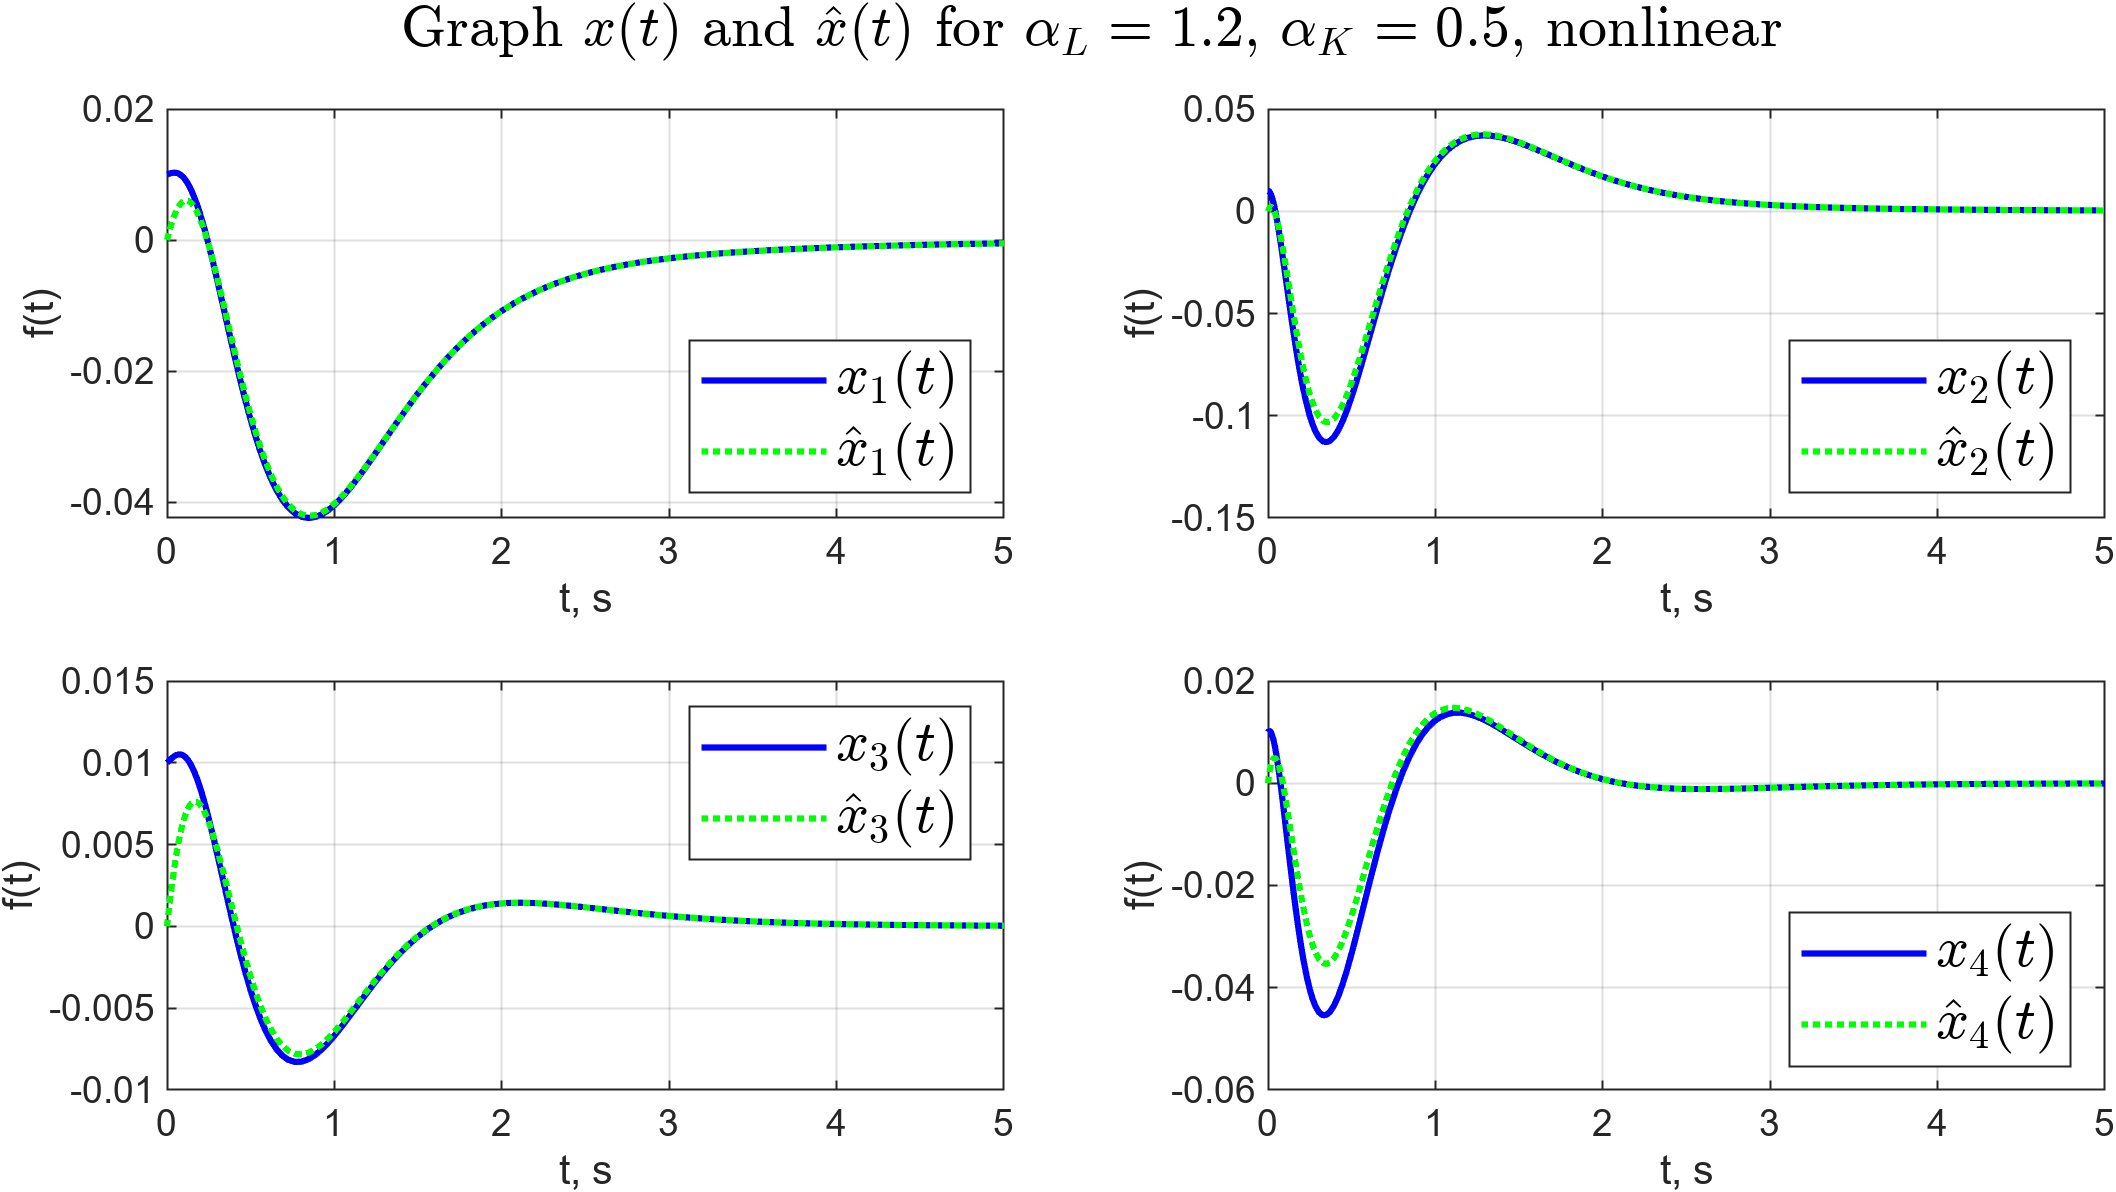
\includegraphics[width=1\linewidth]{pic/4_6_1.20.5x.png}}
	\caption{Графики $\hat{x}(t)$ и $x(t)$, при $\alpha_L = 1.2$ и $\alpha_K = 0.5$.}
	\label{4_6_1.20.5x}
\end{figure}

\begin{figure}[!h]
	\center{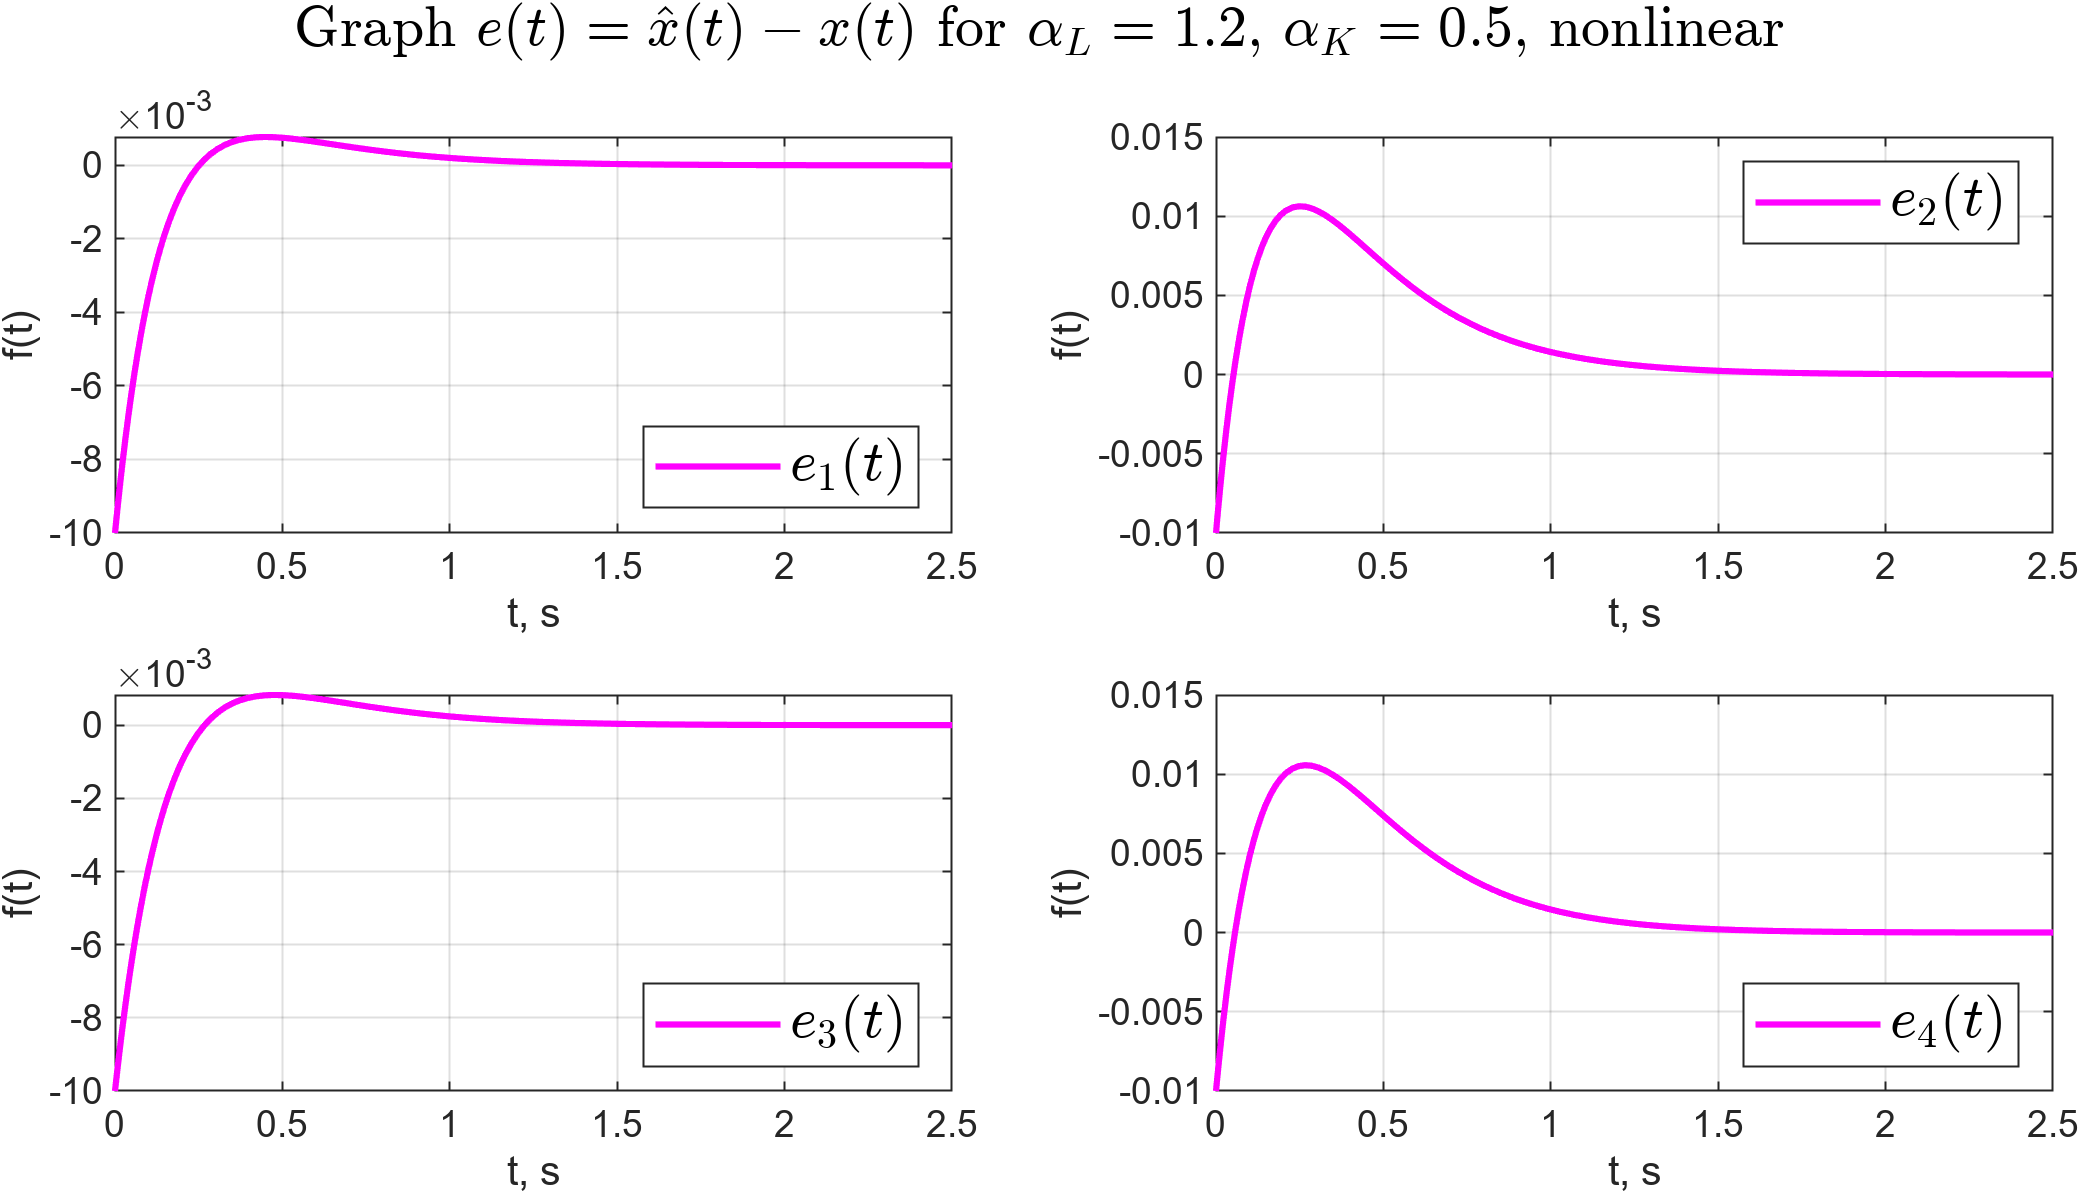
\includegraphics[width=1\linewidth]{pic/4_6_1.20.5e.png}}
	\caption{Графики $e(t) = \hat{x}(t)-x(t)$, при $\alpha_L = 1.2$ и $\alpha_K = 0.5$.}
	\label{4_6_1.20.5e}
\end{figure}

\newpage
Проведем исследование работоспособности построенного регулятора при управлении нелинейной системой (\ref{1_model_full}) в зависимости от выбранных степеней устойчивости. Зададимся наборами степеней устойчивости (таблица \ref{4_tab_6}) и выполним моделирование (рисунки \ref{4_6_0.50.5x}-\ref{4_6_55e}). Время  переходного процесса $t$ (как последний момент времени, когда координата тележки или угол отклонения маятника отличался от нуля более, чем на 0.001), время $t_e$ -- последний момент времени, когда ошибка координаты тележки или угла отклонения маятника  отличался от нуля более, чем на 0.001.

\begin{table}[!h]
	\centering
	\caption{Результаты моделирования при разных значениях параметров $\alpha_K$ и $\alpha_L$.}
	\label{4_tab_6}
	\begin{tabular}{ccccccc}
		\toprule
		$\alpha_K$ & $\alpha_L$ & $\max |\varphi|$ & $\max |a|$  & $t_e$ & $t$ \\
		\midrule
		0.5  &  0.5  &  0.011  &  0.085 & 3.35 & 8.16  \\
		0.5  &  5  &  0.01  &  0.03 & 0.41 & 5.78  \\
		5 &  0.5  &  0.01  &  0.03 & 3.34 & 5.49   \\
		5  &  5  &  0.04  &  0.08 & 0.42 & 1.64 \\
		\bottomrule
	\end{tabular}
\end{table}




\begin{figure}[!h]
\center{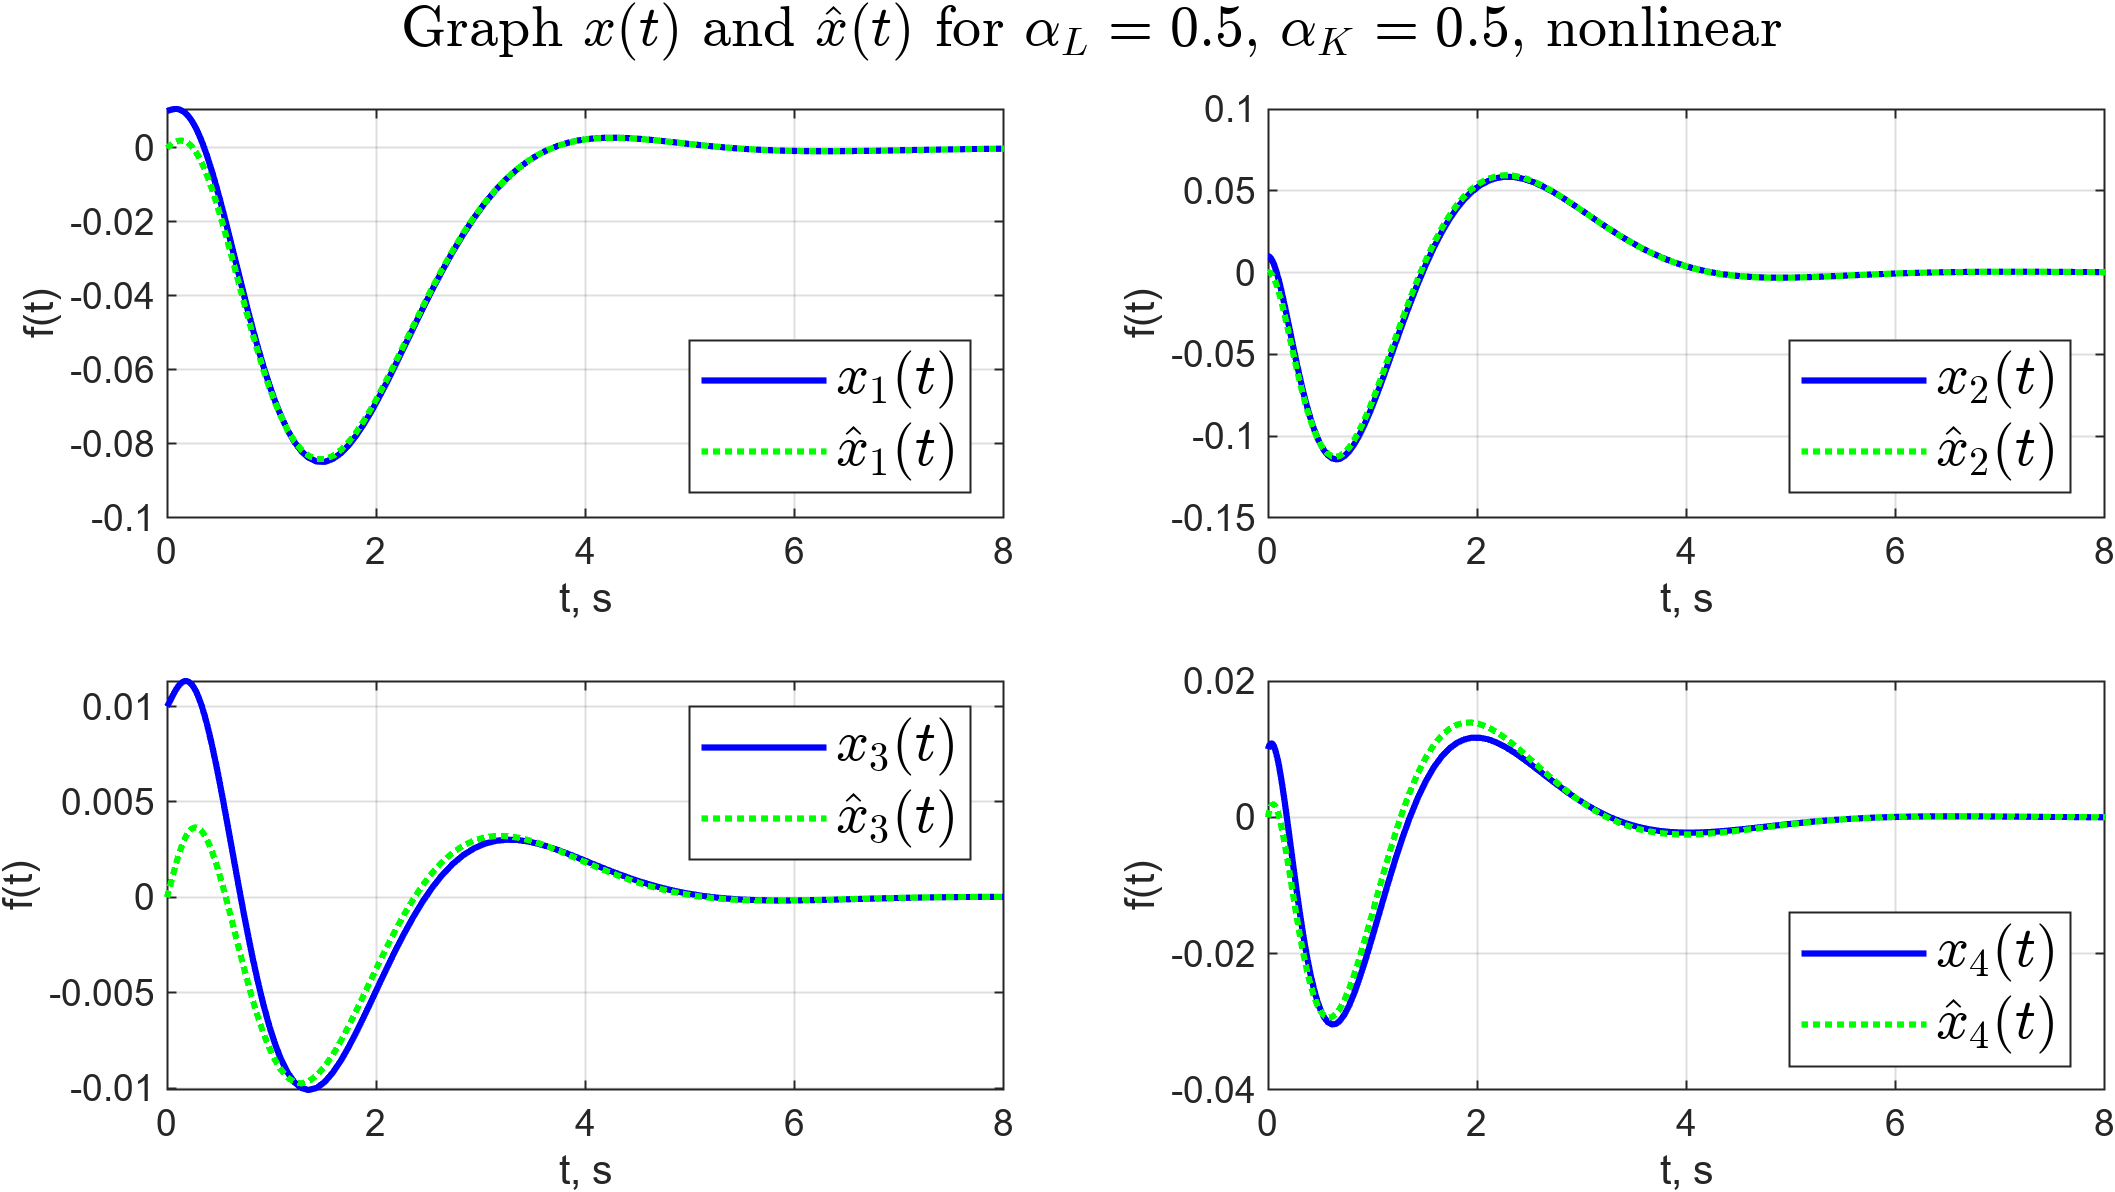
\includegraphics[width=1\linewidth]{pic/4_6_0.50.5x.png}}
\caption{Графики $\hat{x}(t)$ и $x(t)$, при $\alpha_L = 0.5$ и $\alpha_K = 0.5$.}
\label{4_6_0.50.5x}
\end{figure}

\begin{figure}[!h]
\center{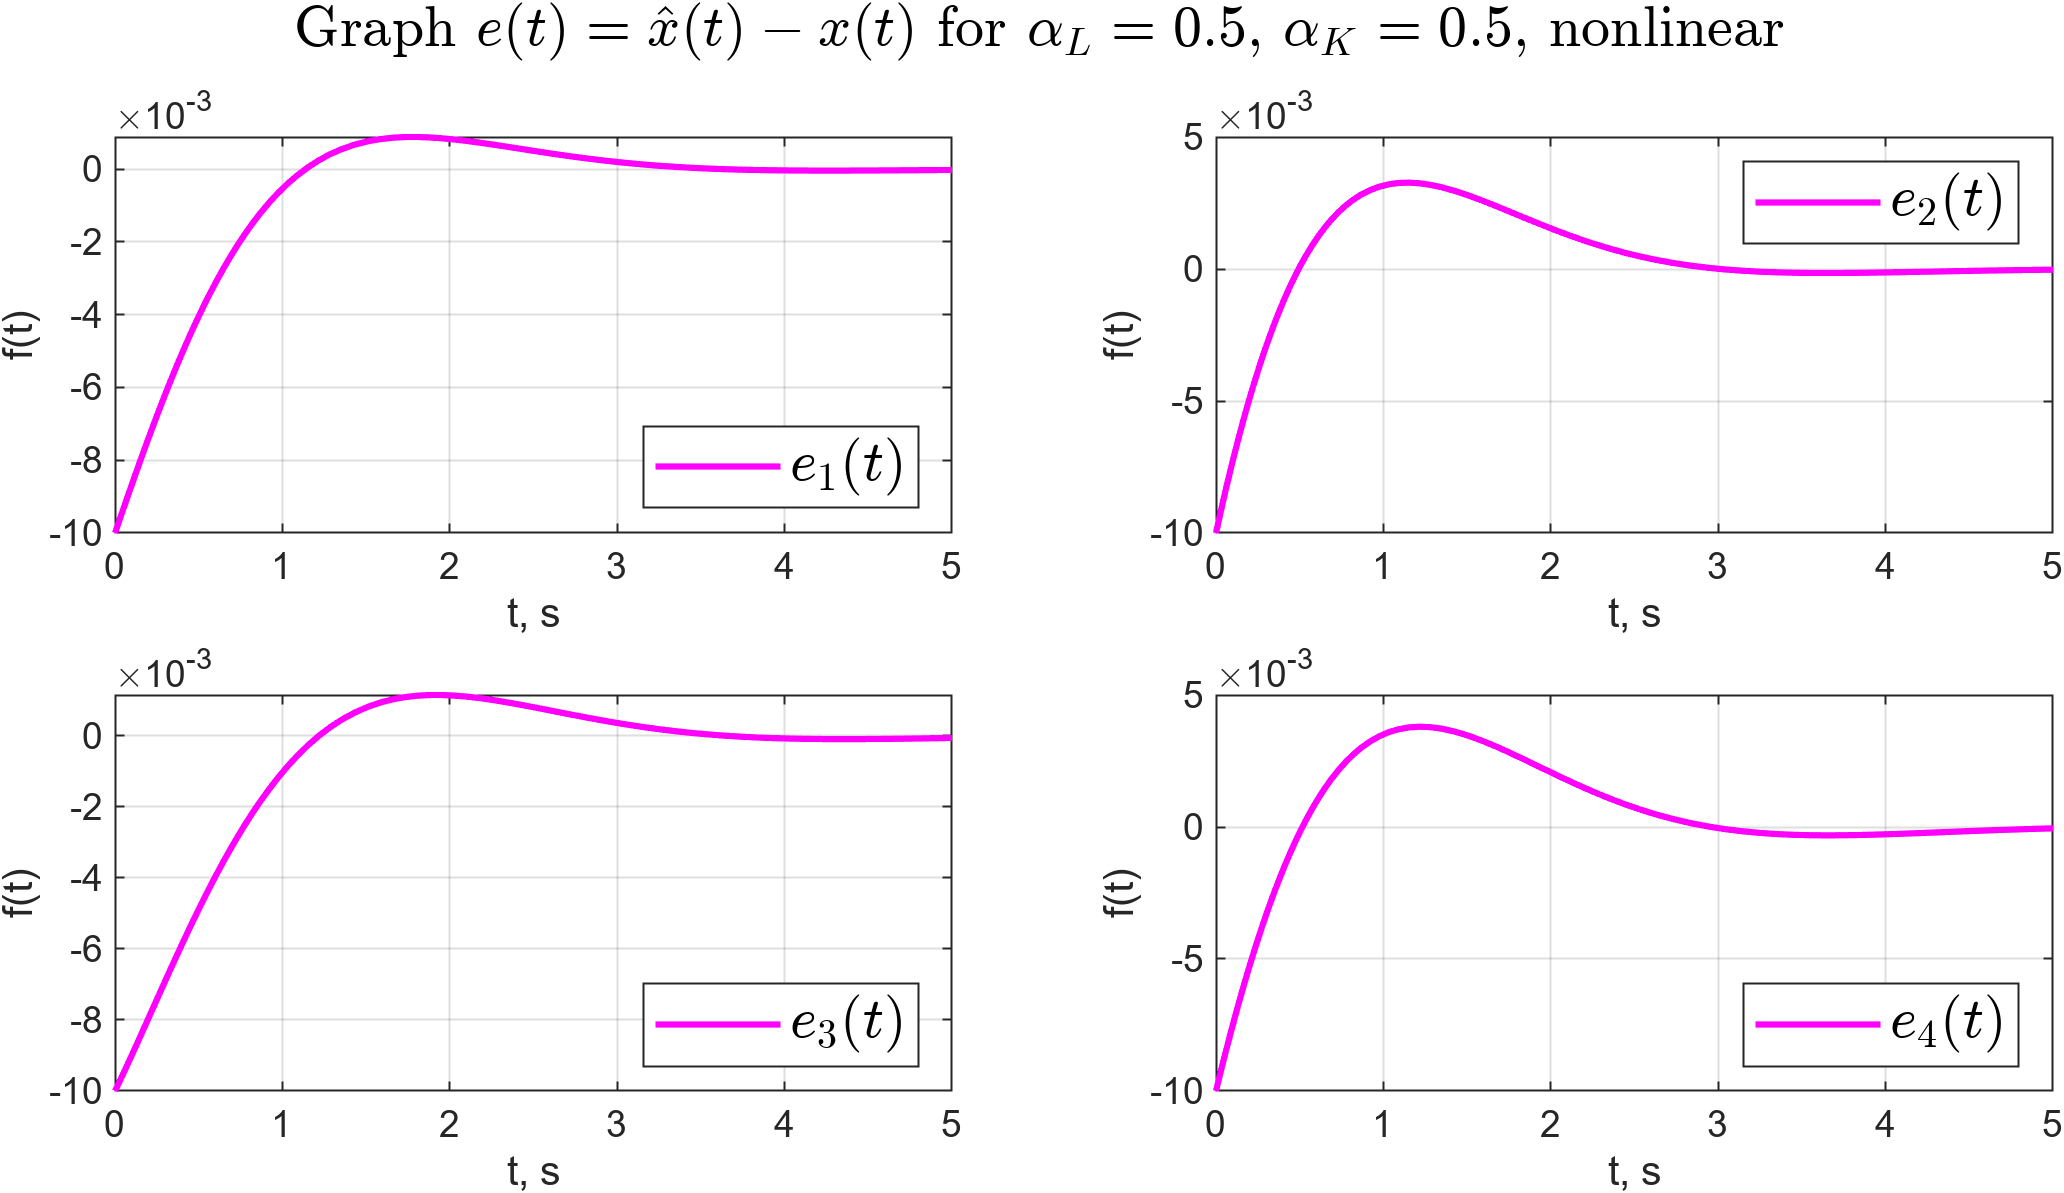
\includegraphics[width=1\linewidth]{pic/4_6_0.50.5e.png}}
\caption{Графики $e(t) = \hat{x}(t)-x(t)$, при $\alpha_L = 0.5$ и $\alpha_K = 0.5$.}
\label{4_6_0.50.5e}
\end{figure}


\begin{figure}[!h]
\center{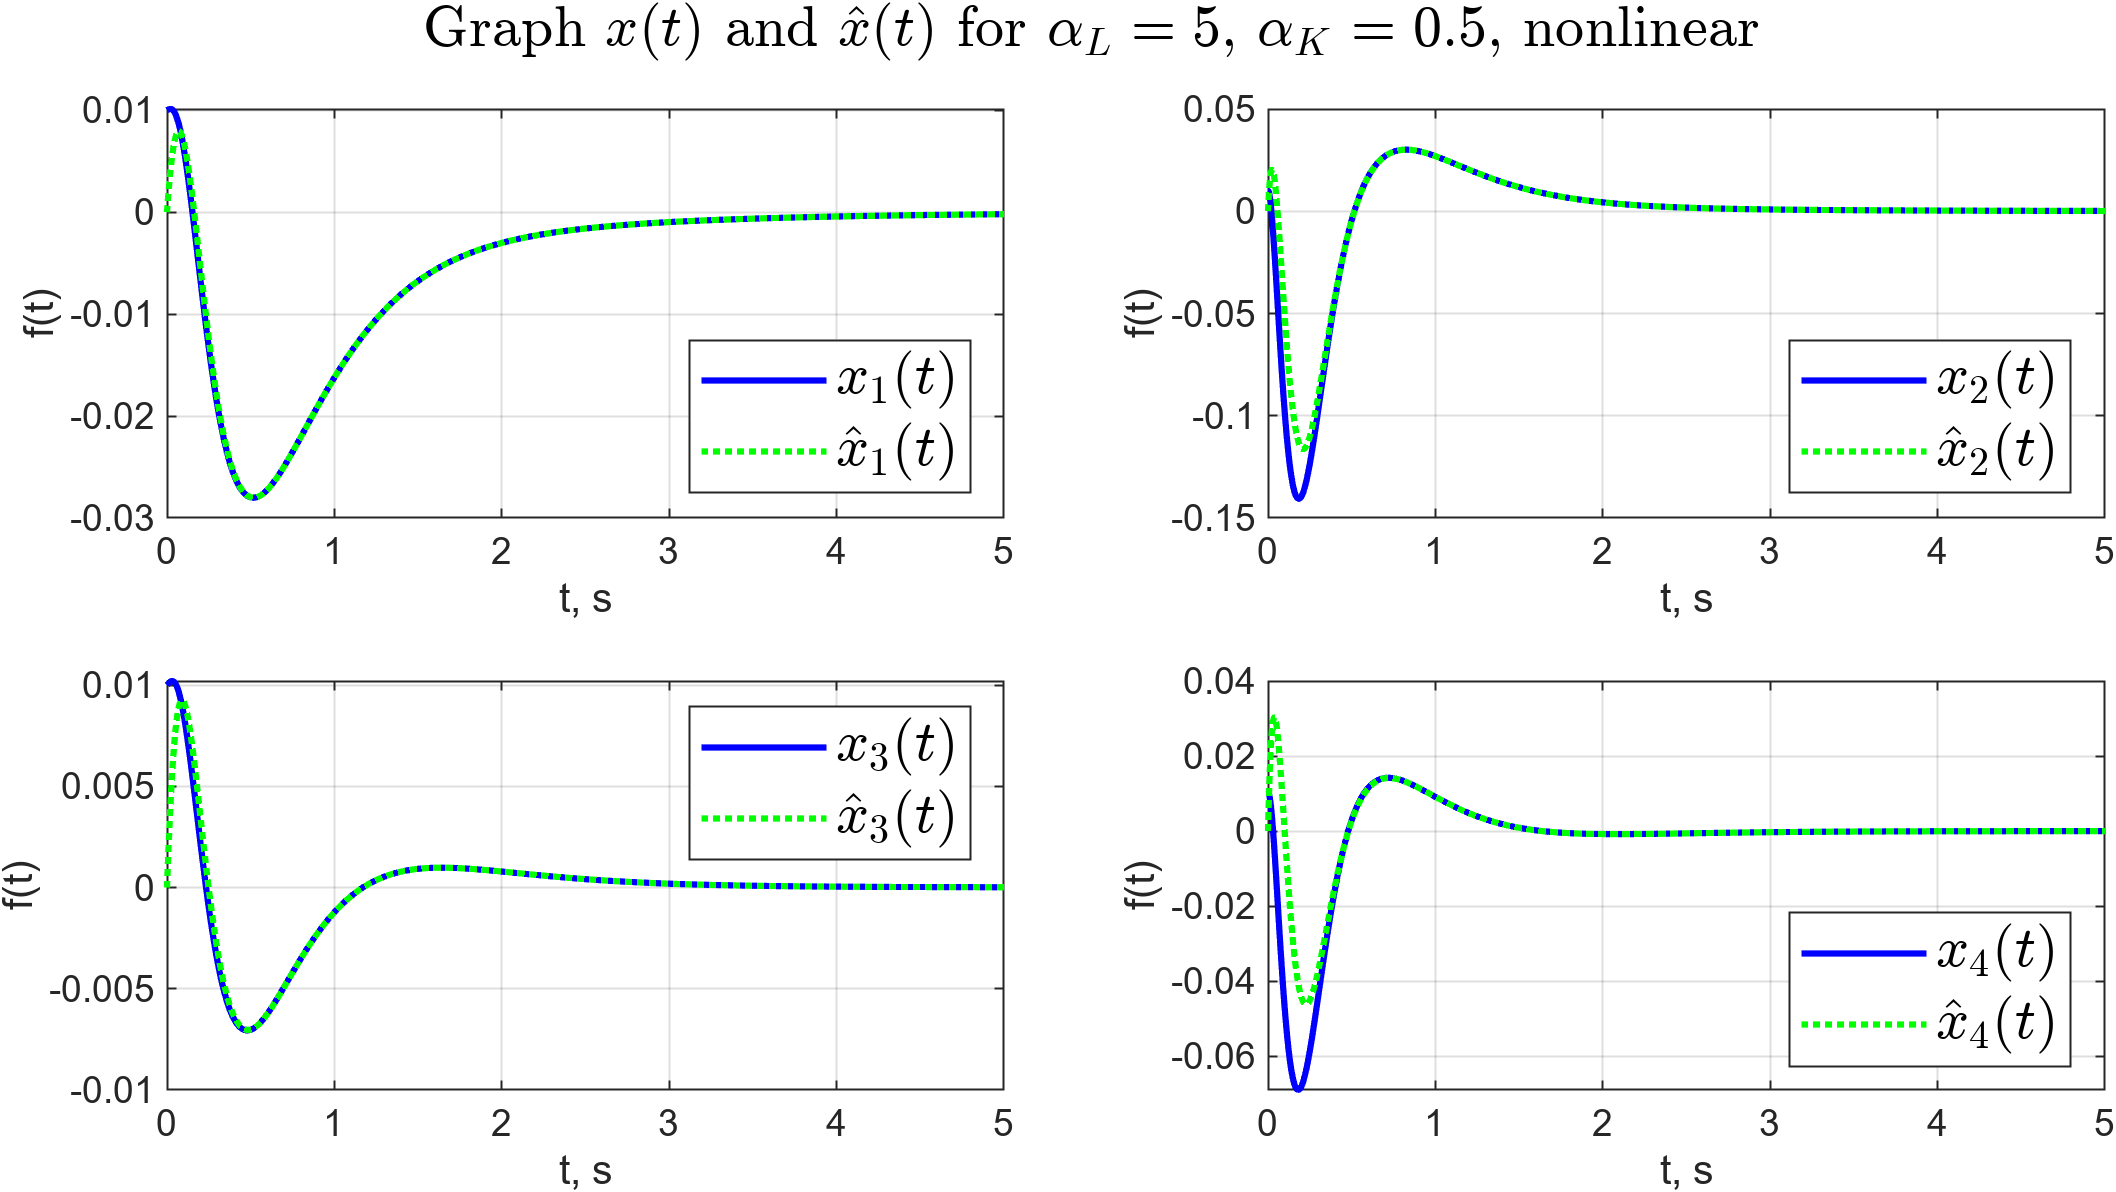
\includegraphics[width=1\linewidth]{pic/4_6_50.5x.png}}
\caption{Графики $\hat{x}(t)$ и $x(t)$, при $\alpha_L = 5$ и $\alpha_K = 0.5$.}
\label{4_6_50.5x}
\end{figure}

\begin{figure}[!h]
\center{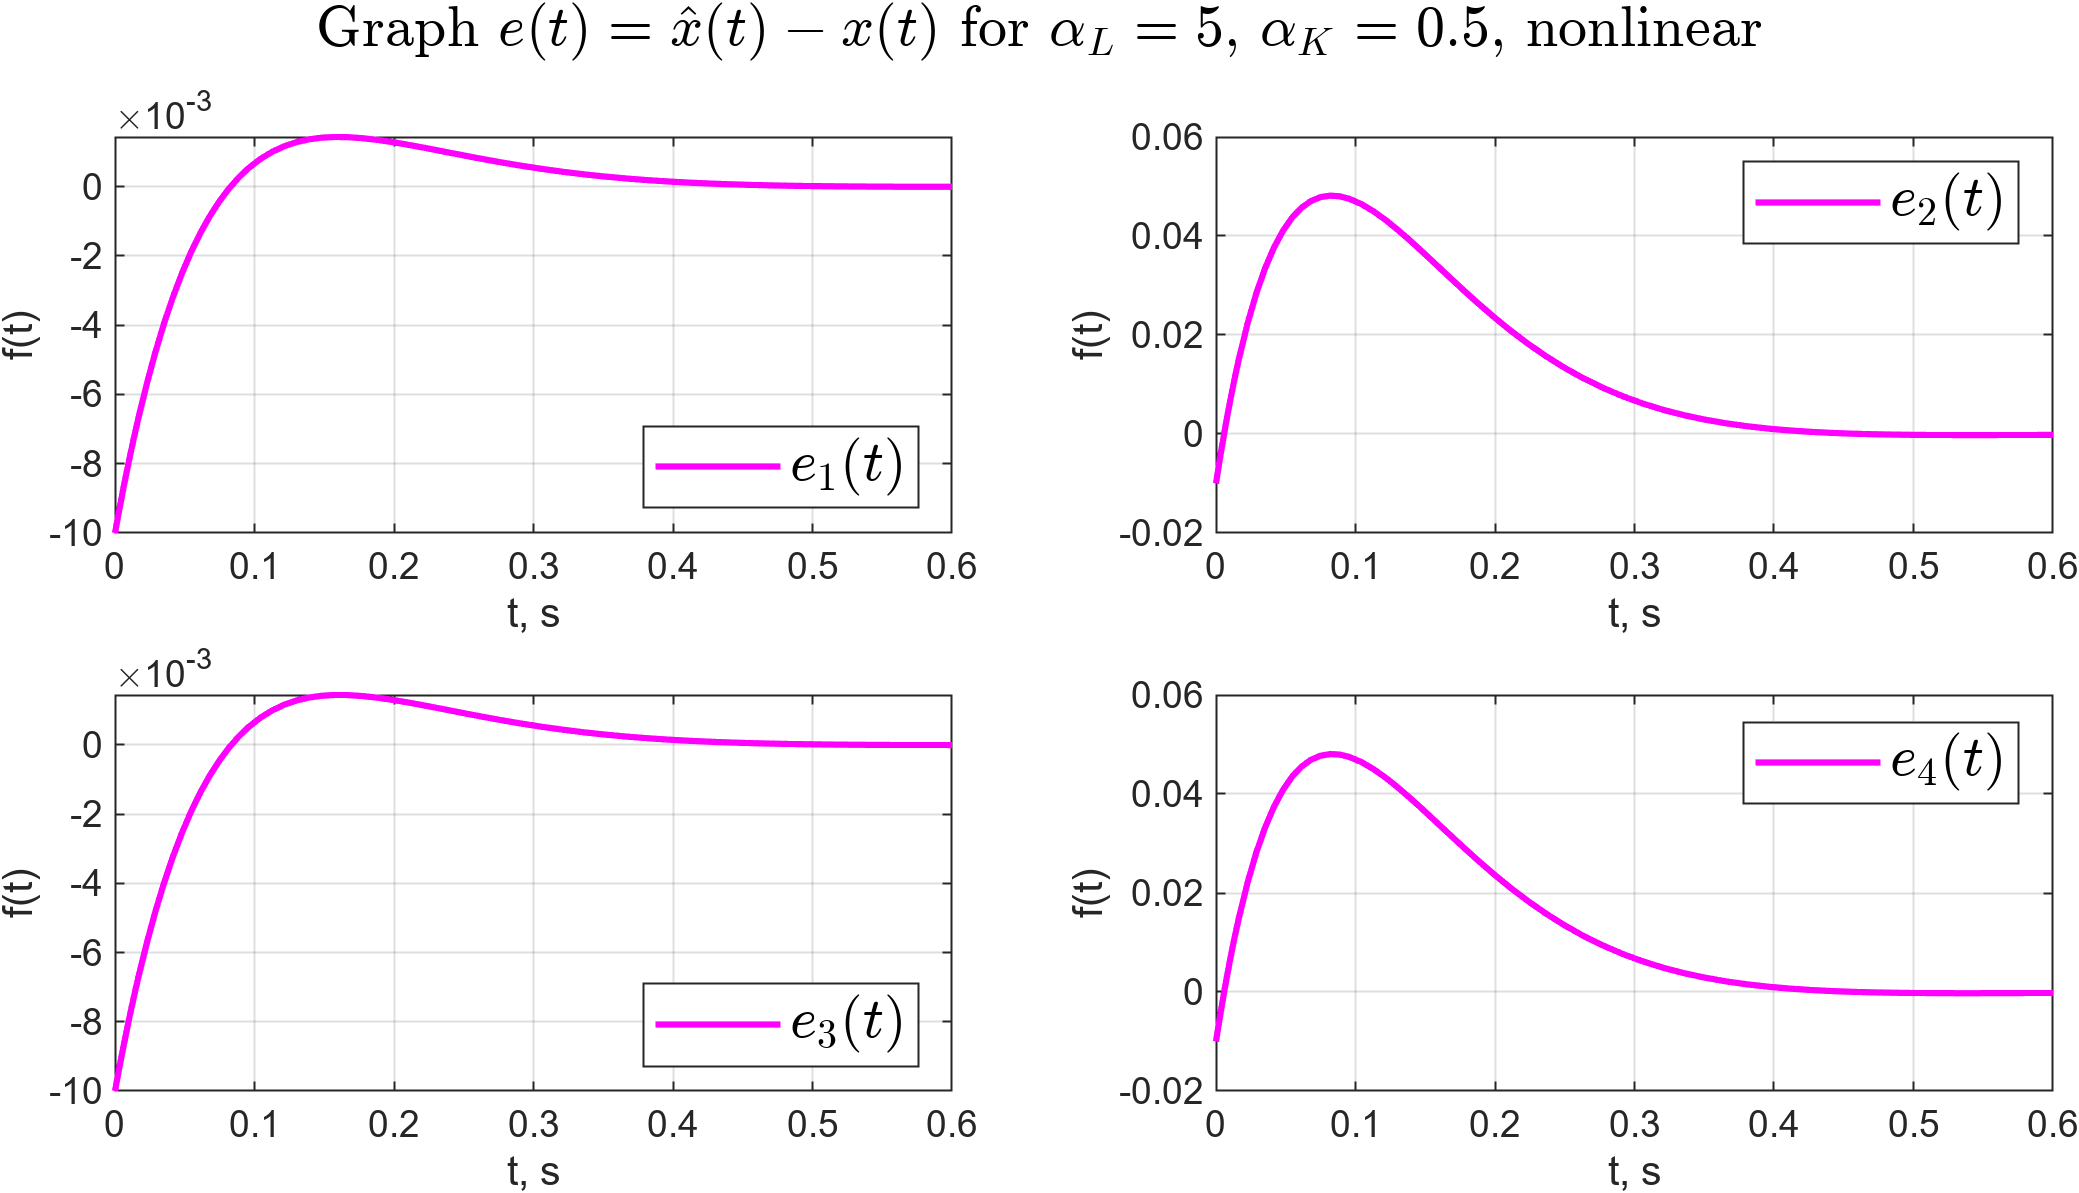
\includegraphics[width=1\linewidth]{pic/4_6_50.5e.png}}
\caption{Графики $e(t) = \hat{x}(t)-x(t)$, при $\alpha_L = 5$ и $\alpha_K = 0.5$.}
\label{4_6_50.5e}
\end{figure}


\begin{figure}[!h]
\center{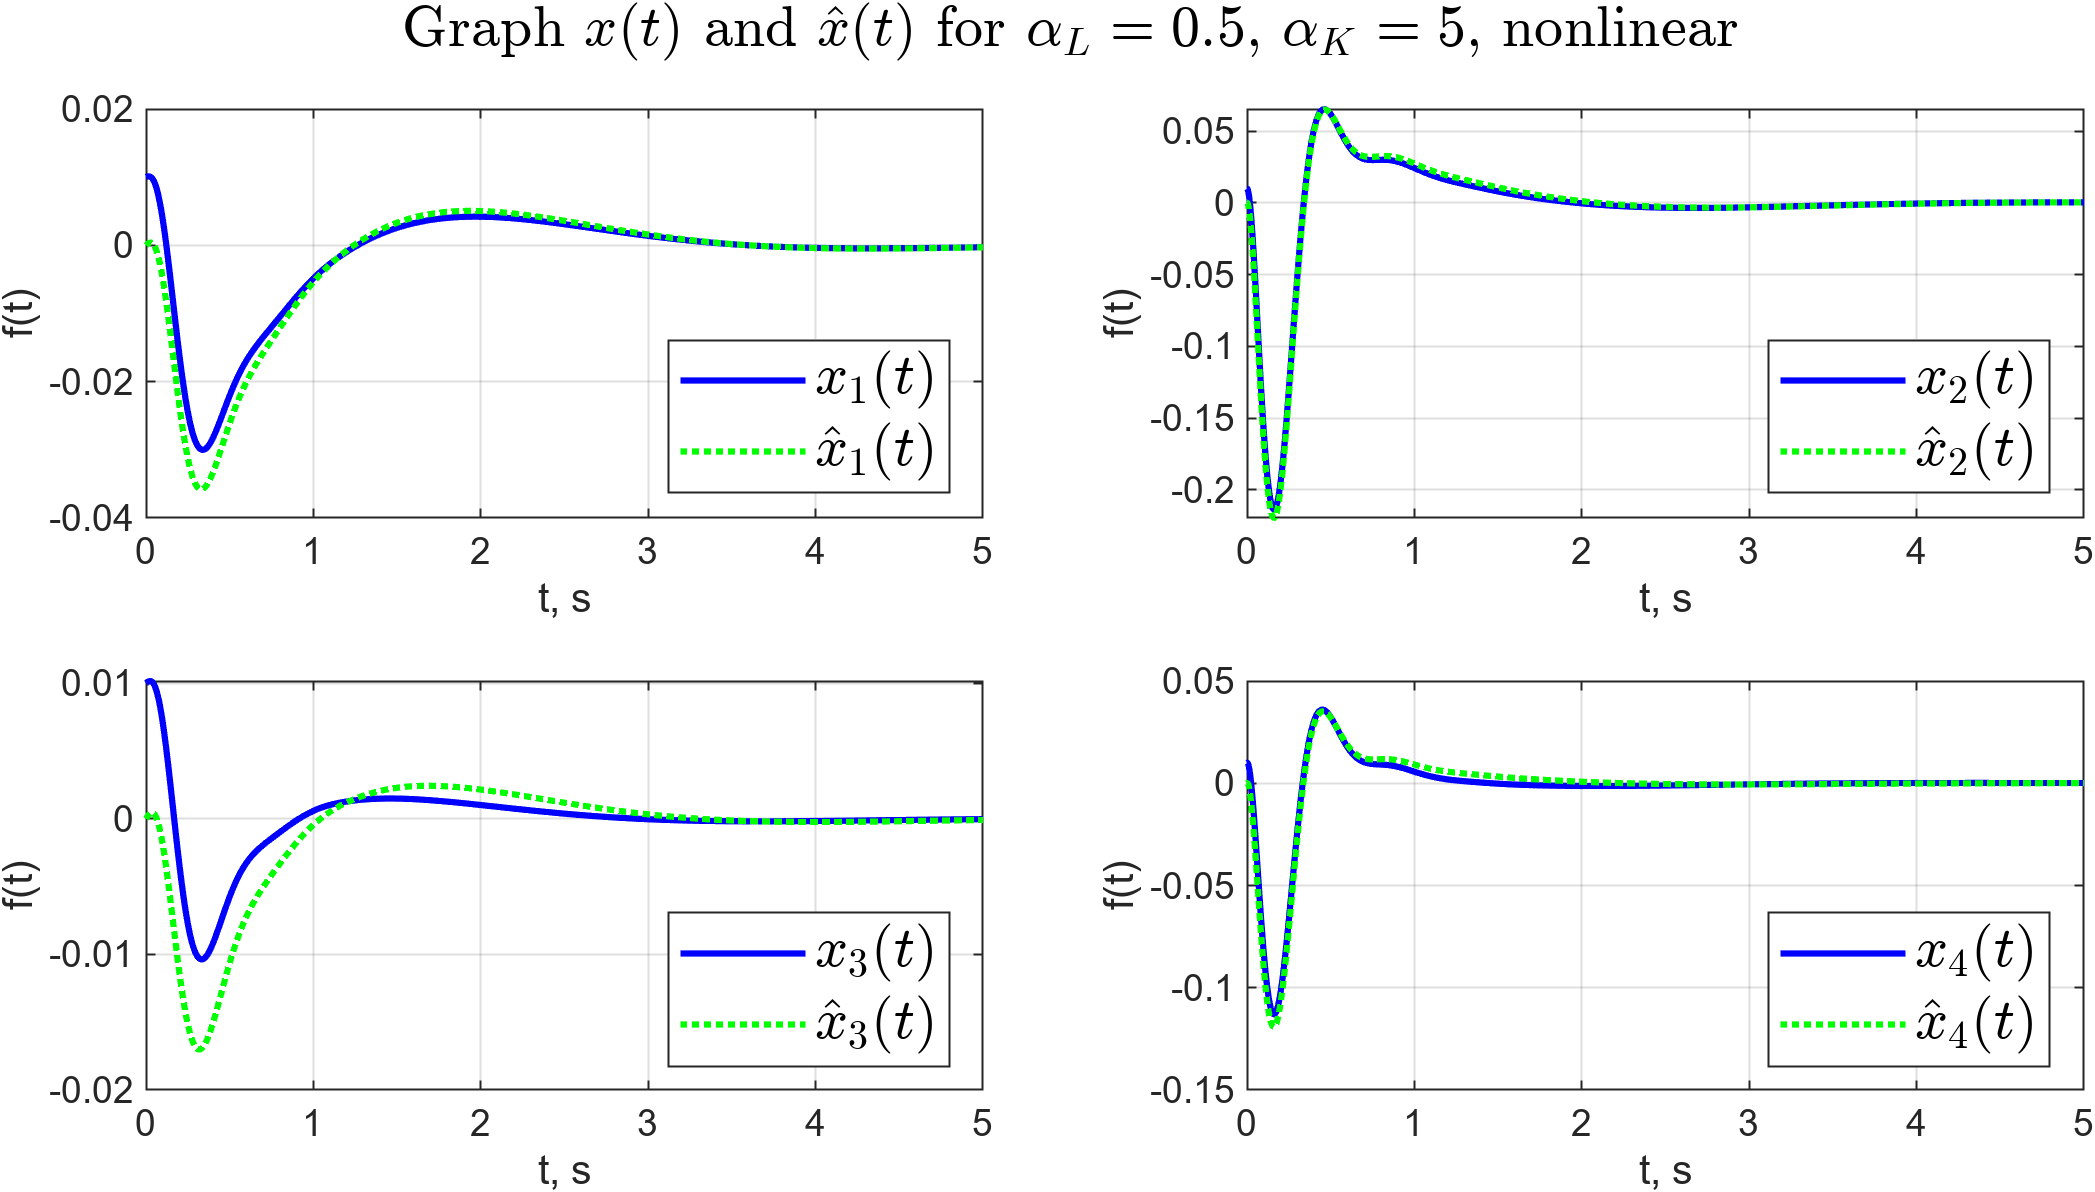
\includegraphics[width=1\linewidth]{pic/4_6_0.55x.png}}
\caption{Графики $\hat{x}(t)$ и $x(t)$, при $\alpha_L = 0.5$ и $\alpha_K = 5$.}
\label{4_6_0.55x}
\end{figure}

\begin{figure}[!h]
\center{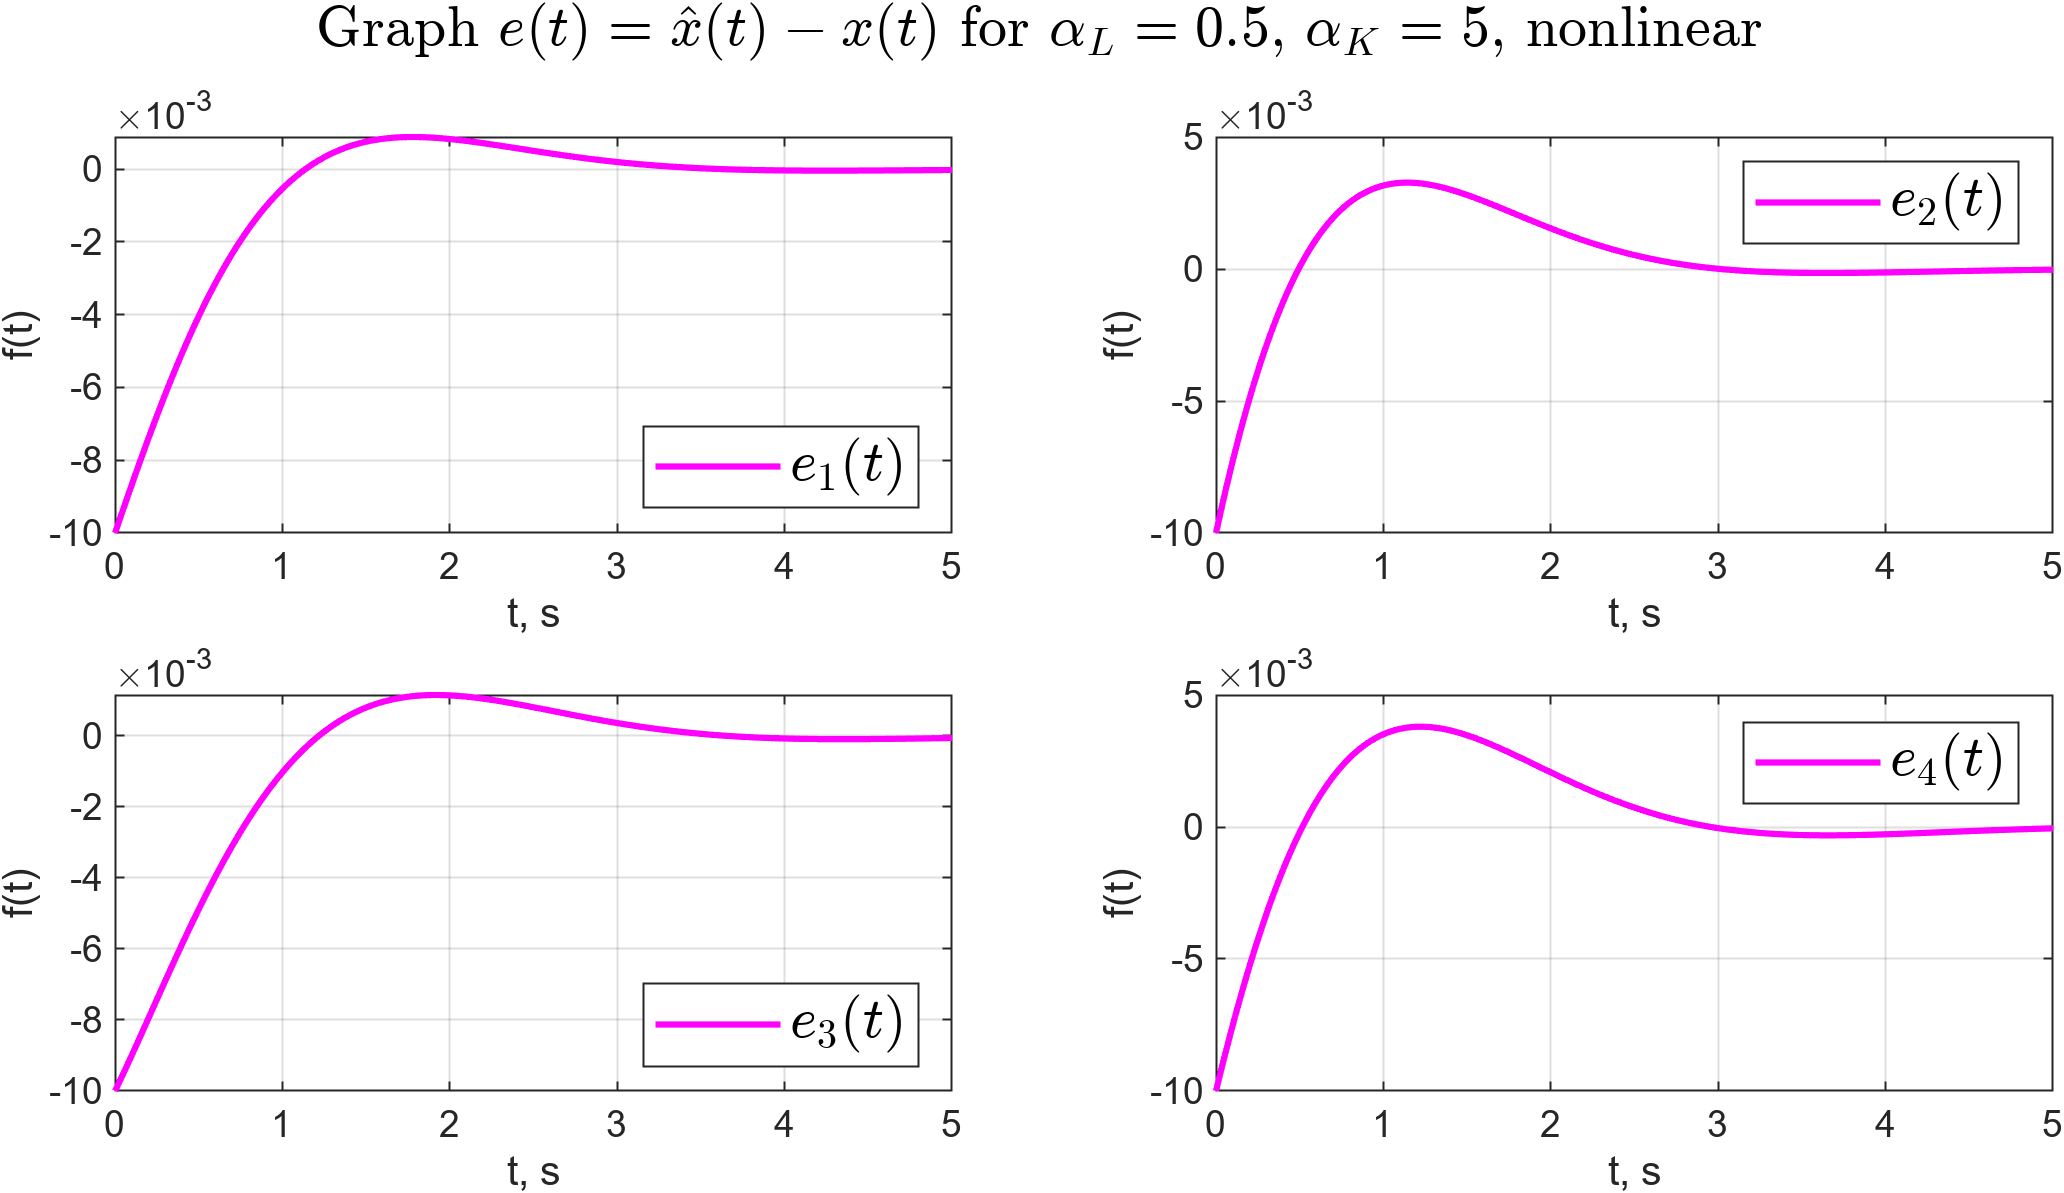
\includegraphics[width=1\linewidth]{pic/4_6_0.55e.png}}
\caption{Графики $e(t) = \hat{x}(t)-x(t)$, при $\alpha_L = 0.5$ и $\alpha_K = 5$.}
\label{4_6_0.55e}
\end{figure}


\begin{figure}[!h]
\center{\includegraphics[width=1\linewidth]{pic/4_6_55x.png}}
\caption{Графики $\hat{x}(t)$ и $x(t)$, при $\alpha_L = 5$ и $\alpha_K = 5$.}
\label{4_6_55x}
\end{figure}

\begin{figure}[!h]
\center{\includegraphics[width=1\linewidth]{pic/4_6_55e.png}}
\caption{Графики $e(t) = \hat{x}(t)-x(t)$, при $\alpha_L = 5$ и $\alpha_K = 5$.}
\label{4_6_55e}
\end{figure}

\newpage
\,
\newpage
\,
\newpage
\,
\newpage
Как можно заметить для различных комбинаций значений степеней устойчивости $0.5$ и $5$ регулятор по выходу справляется с задачей стабилизации. Чем выше $\alpha_L$, тем быстрее ошибка между $\hat{x}(t)$ и $x(t)$ сходится к нулю ($0.41$-$0.42$ секунды для $\alpha_L= 5$ и $3.34$-$3.35$ секунды для $\alpha_L= 0.5$), сочетание большого значения $\alpha_{L,K}=5$ приводит к меньшему времени стабилизации системы, но к большей аплитуде координаты тележки и угла отклонения маятника от вертикали.


\endinput